\documentclass[prodmode,acmtods]{acmsmall}
\pdfminorversion=6

%Metadata Information
\acmVolume{1}
\acmNumber{1}
\acmArticle{1}
\acmYear{2017}
\acmMonth{8}

\usepackage{url}
\usepackage{algorithm}
\usepackage{algorithmic}
\usepackage{graphics}
% \usepackage[total={6.5in,9in}, top=1.25in,left=0.9in]{geometry}
%\usepackage[text={6.5in,9in},centerpage,includefoot]{geometry}
% \usepackage{setspace}
\usepackage{color}
\usepackage{url}
\usepackage{balance}
\usepackage{amsmath}
\usepackage{amssymb}
\usepackage{subfigure}
\usepackage{nicefrac}

\definecolor{grey}{RGB}{200,200,200}
\newcommand{\hilite}[1]{\colorbox{grey}{#1}}
\newcommand{\hilitey}[1]{\colorbox{yellow}{#1}}
\newcommand{\hiliting}[1]{\colorbox{grey}{#1}}
\long\def\todo#1{\hilitey{{\bf TODO:} {\em #1}}}
\long\def\shorten#1{}

%For last edit: revise and resubmit for SIGMOD'14
\long\def\shortenF#1#2{}%First is letter indicating what has been removed

%For double blind, keep the second argument. To turn off doubleblind, keep
%the first
\long\def\doubleblind#1#2{#2}
%To remove discontinuity, keep the second argument. To include discontinuity,
%keep the first argument
\long\def\discont#1#2{#2}
\def\azdb{\doubleblind{\hbox{\sc AZDBLab}}{\hbox{\sc DBLab}}}
\def\QatC{Q{@}C}
\long\def\comment#1{}
%c2j: Conference to Journal: first parameter is conference, second is journal
% For Conferences: c2j#1#2{#1}
% For Journals: c2j#1#2{2}
\long\def\c2j#1#2{#2}

\begin{document}

\title{%\vspace*{-0.75in}
A Causal Model of \hbox{DBMS} Suboptimality\\
}
\markboth{\ }{A Causal Model of \hbox{DBMS} Suboptimality}


% possible, but not really needed or used for PVLDB:
%\subtitle{[Extended Abstract]
%\titlenote{A full version of this paper is available as\textit{Author's Guide to Preparing ACM GIG Proceedings Using \LaTeX$2_\epsilon$\ and BibTeX} at \texttt{www.acm.org/eaddress.htm}}}

% ****************** AUTHORS **************************************

% You need the command \numberofauthors to handle the 'placement
% and alignment' of the authors beneath the title.
%
% For aesthetic reasons, we recommend 'three authors at a time'
% i.e. three 'name/affiliation blocks' be placed beneath the title.
%
% NOTE: You are NOT restricted in how many 'rows' of
% "name/affiliations" may appear. We just ask that you restrict
% the number of 'columns' to three.
%
% Because of the available 'opening page real-estate'
% we ask you to refrain from putting more than six authors
% (two rows with three columns) beneath the article title.
% More than six makes the first-page appear very cluttered indeed.
%
% Use the \alignauthor commands to handle the names
% and affiliations for an 'aesthetic maximum' of six authors.
% Add names, affiliations, addresses for
% the seventh etc. author(s) as the argument for the
% \additionalauthors command.
% These 'additional authors' will be output/set for you
% without further effort on your part as the last section in
% the body of your article BEFORE References or any Appendices.

%bug is vldb.cls gives an additional authors section for greater than 3...
\doubleblind{\numberofauthors{3}}{}
 %  in this sample file, there are a *total*
% of EIGHT authors. SIX appear on the 'first-page' (for formatting
% reasons) and the remaining two appear in the \additionalauthors section.


\author{
% You can go ahead and credit any number of authors here,
% e.g. one 'row of three' or two rows (consisting of one row of three
% and a second row of one, two or three).
%
% The command \alignauthor (no curly braces needed) should
% precede each author name, affiliation/snail-mail address and
% e-mail address. Additionally, tag each line of
% affiliation/address with \affaddr, and tag the
% e-mail address with \email.
%
\doubleblind{% 1st. author
Richard T.~Snodgrass\\
       \affaddr{Dept. of Computer Science}\\
       \affaddr{University of Arizona}\\
%       \affaddr{Tucson, AZ}\\
       \email{\small\tt rts@cs.arizona.edu}
\alignauthor
% 2nd. author
\alignauthor
Sabah Currim\\
       \affaddr{Alumni Office}\\
       \affaddr{University of Arizona}\\
%       \affaddr{Tucson, AZ}\\
%       %\vspace*{-0.05in}
       \email{\small\tt scurrim@email.arizona.edu}
% 3rd. author
\alignauthor
Young-Kyoon Suh\\
       \affaddr{Dept. of Computer Science}\\
       \affaddr{University of Arizona}\\
%       \affaddr{Tucson, AZ}\\
       \email{\small\tt yksuh@cs.arizona.edu}
}{}}

\begin{abstract}

The query optimization phase within a database management system (\hbox{DBMS}) ostensibly finds the fastest query
execution plan from a potentially large set of enumerated plans, all of
which correctly compute the specified query. Occasionally the cost-based optimizer
selects a slower plan, for a variety of reasons. We introduce the notion of
{\em empirical suboptimality} of a query plan chosen by the DBMS,
indicated by the existence of a query plan that performs more efficiently
than the chosen plan, for the same query. From an engineering
perspective, it is of critical importance to understand the prevalence
of suboptimality and its causal factors.

We propose a novel structural causal model to explicate the relationship
between various factors in query optimization and empirical
suboptimality. Our model associates suboptimality with the factors of
complexity of the schema, data, query, and optimizer and concomitant
interactions among the components of the optimizer. This model induces a
number of specific hypotheses that were subsequently tested on multiple
\hbox{DBMSes}.

Through a series of experiments that examine the plans for thousands of
queries run on one hundred thousand query/cardinality combinations on four
popular DBMSes, we observe that the dependent construct of empirical
suboptimality prevalence correlates positively with (a)~\hbox{DBMS}
complexity, (b)~schema complex, (c)~data complexity, and (d)~query
complexity, providing empirical support for this model. These
\discont{ten}{nine} factors explain in concert over half of the
variance of suboptimality, across four disparate DBMSes. Thus, it is the
common aspects of these DBMSes that predict
suboptimality, {\em not} the particulars embedded in the inordinate complexity of
each of these DBMSes.

An implication of this causal model is that as query evaluation operators
are added to a DBMS, the prevalence of slower queries will grow. Through a
novel experiment that examines the plans on the afore-mentioned
query/cardinality combinations, we present evidence for a previously-unknown
upper bound on the number of operators a DBMS may be able to support before
performance suffers.  We
show that this upper bound may have already been reached by one or more
extant~DBMSes.

This paper thus provides a new methodology to study mature query optimizers, that
of empirical generalization, proposes a novel causal model for empirical query
suboptimality, and demonstrates an upper bound that may have already
been encountered, with implications for fundamental improvements of those
cost-based query optimizers.
\end{abstract}

% A category with the (minimum) three required fields
%\category{H.4}{Information Systems Applications}{Miscellaneous}
%A category including the fourth, optional field follows...
%\category{D.2.8}{Software Engineering}{Metrics}[complexity measures,
%performance measures]
\terms{}
\keywords{}
\acmformat{\doubleblind{Richard T.~Snodgrass, Sabah Currim, and Young-Kyoon
    Suh, 2017, A Causal Model of \hbox{DBMS} Suboptimality}{A Causal Model of
    \hbox{DBMS} Suboptimality}}

\doubleblind{\begin{bottomstuff}
This work was supported in part by NSF grants \hbox{IIS-0639106},
IIS-0415101, and EIA-0080123. 
%
%Author's addresses: G. Zhou, Computer Science Department,
\end{bottomstuff}}{}
\maketitle

\section{Introduction}\label{sec:intro}
Database management systems (DBMSes) underlie information systems and hence optimizing their performance is of
critical importance. A relational DBMS's cost-based query optimizer plays an
important role, ostensibly finding a fast query execution plan from a
potentially large set of possible plans, all of which correctly compute the
submitted query, using a cost model that references properties of the
underlying relations. But
what if the optimizer {\em doesn't}: what if it selects a slow plan?

This paper provides a thorough investigation into \hbox{DBMS}
suboptimality: when the \hbox{DBMS} chooses a slower plan over a faster
plan for a given query. We systematically examine the factors influencing
the number of suboptimal queries. There could be multiple causes of the
suboptimality. One possible cause could be some peculiarity within the tens
of thousands of lines of code of that query optimizer. Another possible
cause could be the query's complexity. Prior research in other domains shows
that increasing complexity negatively influences
performance~\cite{campbell88,moody98}. A third possible reason could be some
fundamental limitation {\em within the general architecture of cost-based
  optimization} that will always render a number of queries suboptimal.

To better understand the impact of different factors on suboptimality of
query performance and the relationship between operators, especially in a
dynamic environment, an experimental approach is needed.  Based on existing
research and general knowledge of \hbox{DBMSes}, we propose an innovative
predictive model of suboptimality in query evaluation. From this point on,
by ``suboptimality'' we mean specifically ``empirical suboptimality'',
indicated by the presence of another plan that can be empirically determined
to be faster than the plan that was chosen by the query optimizer. Indeed,
as we will elaborate in Section~\ref{sec:suboptimality}, where we provide a
specific operationalization of this notion, empirical suboptimality is an
{\em ordinal variable}, indicating the degree to which plans across a
range of table cardinalities are slower than other (empirically-identified)
plans. This contrasts with the conventional notion of query plan
suboptimality, which is a binary {\em categorical variable} associated with
a particular cardinality: a plan is either optimal (the best-performing
plan) or it is suboptimal.

We employ an experimental methodology on a collection of \hbox{DBMSes} as
subjects to test our hypotheses with respect to factors influencing
suboptimality, utilizing empirical data collected over a \hbox{cumulative}
16,000 hours (over two years) of query executions.  Our research falls
within creative development of new evaluation methods and metrics for
artifacts, which were identified as important design-science
contributions~\cite{hevner04}.

%\pagebreak
The key contributions of this paper are as follows.
\begin{itemize} 
\item We use an innovative {\em methodology} that treats \hbox{DBMSes} as experimental subjects.

\item We find that for a surprisingly large portion of queries, the plan
  chosen  by the query optimizer is not the best plan, for some cardinality
  of the underlying tables.

\item We propose a {\em predictive model} for \hbox{DBMSes} to better
  understand the factors causing suboptimality.

\item We test the six quite specific hypotheses that arise from that
  model across a wide range of DBMSes, queries, and data, showing
  through correlational and regression analyses that four
  hypotheses are strongly supported, one is weakly in the
  other direction, and
  the sixth is partially supported, lending credibility to our particular model.

\item Through an innovative
  analysis, we track the net cumulative benefit of a succession of operators
  added to the DBMS, and show (a)~that there is a {\em limit} to the number of
  relational operators that a DBMS can accommodate before slower plans start
  to dominate and (b)~that one or more extant relational DBMSes may have
  already reached that limit.

\item The predictive model and these experimental results suggest several specific
  engineering~directions.

\item The model and analyses presented here taken as a whole imply that a
  new approach to query optimization, fundamentally
  different from the cost-based approach utilized over the last forty years, may be required
  to get past the fundamental limitation uncovered in this research.
\end{itemize}

This paper takes a scientifically rigorous approach to an
area previously dominated by the engineering perspective, that of database
query optimization.  Our goal is to \hbox{understand} cost-based query optimizers
as a {\em general} class of computational artifacts and to come up with
insights and ultimately with predictive theories about how such optimizers,
again, as a general class, behave.  These theories can be used to further
improve \hbox{DBMSes} through engineering \hbox{efforts} that benefit from the fundamental
understanding that the scientific perspective can provide.

One might ask, shouldn't the task of optimizing queries be left to DBAs?  In
databases, and especially in data warehouses, the number of users writing
and running queries has been growing exponentially. This growth is aided, in
part, by the drag and drop query tools provided by the different
systems. For example, subject areas allow business users to write queries
without knowing anything about the underlying database structure. This,
coupled with constantly growing data presents new challenges for tuning. For
example, \doubleblind{the data warehouse deployed at the University of
  Arizona}{a large data warehouse we are familiar with} runs about
30,000 queries on a daily basis. 
Also, tuning a subject area or tables for one group of queries can
negatively impact the performance of other queries. Query optimization experts often take hours to tune and test existing canned
queries; the amount expended on this one system for manual query optimization
approaches \$100K/year. Therefore, we argue that it is important to
understand how existing query optimizers can be further improved, and
indeed, whether  fundamental limitation inherent in these optimizers exist
and whether such limitations are indeed already being encountered.

We focus here on the effectiveness of query
optimization. The query optimization phase within a \hbox{DBMS} ostensibly
finds a fast query execution plan, drawn from a potentially large set of enumerated plans, all of
which correctly compute the specified query. (The term ``query optimizer'' is thus aspirational rather
than realistic: the goal of the optimizer isn't really to find the best
plan, but rather to avoid the worst plans.) However, this intermediate goal
might not always be realized in practice, for several possible reasons. One is
that it may not be practical to enumerate all possible plans, and so the
fastest plans, or even the fast plans, may not be considered. Also, because
the optimizer chooses a plan based on its estimated query execution time, if
that estimate is of, the optimizer may instead choose a different, less
efficient plan. From both a scientific perspective and an engineering
perspective, it is of critical importance to understand the phenomenon of
suboptimality.

We study these aspects \c2j{}{across \hbox{DBMSes}} to identify the
underlying causes. We have developed a predictive causal model that
identifies five constructs that may play a role in suboptimality. The ultimate goal is to {\em
  understand} a component within a \hbox{DBMS}, its cost-based optimizer, through the
articulation and empirical testing of a general scientific theory.

In Section~\ref{sec:related} we briefly summarize the vast amount of related
work in query optimization to establish the technical basis for our study.
The following section introduces the methodology we will follow, that of
{\em empirical generalization}~\cite{cohenbook}. We present in
Sections~\ref{sec:model} and~\ref{sec:operationalization} a predictive,
causal model of suboptimality and state six specific hypotheses derived
from that model. We then test these hypotheses across a number of queries,
data, and cardinalities, whose results provide strong support for the
validity of the proposed model.  These are the first scientific results that
we are aware of that apply {\em across} multiple \hbox{DBMSes}, rather than on a
single, specific \hbox{DBMS} or on a specific algorithm. In
Section~\ref{sec:diminishing} presents a follow-on analysis that
uncovers a previously-unknown fundamental limit to the number of operators that a
cost-based optimizer can support, and shows that this limit may have already
been reached by one or more extant DBMSes.
We explore in Section~\ref{sec:engineering} implications of the model for
research in engineering more efficient \hbox{DBMSes}.

\section{Motivation}\label{sec:motivation}

Consider a simple select-project-join (SPJ) query, with a few attributes in
the SELECT clause, a few tables referenced in the FROM clause,
and a few equality predicates in the WHERE clause. This query might be an
excerpt from a more complex query, with the tables being intermediate
results.

%%%% query info: runid: 440, dbms: pgsql, querynum:13, exp: op-1M-100q-6
%\vspace*{-2ex}
\noindent
\hspace{3ex}{\small\begin{verbatim}
        SELECT t0.id1, t0.id2, t2.id4, t1.id1 
        FROM ft_HT3 t2, ft_HT2 t1, ft_HT1 t0 
        WHERE t2.id4=t1.id1 AND t2.id1=t0.id1
\end{verbatim}
}

%\vspace*{-2ex}
\noindent
The optimizer generates
different plans for this query as the cardinality of the {\tt
  ft\_HT1} table varies, an experiment that we will elaborate later in depth.

The upper graph in Figure~\ref{fig:query769} represents the plans chosen by
a common DBMS as the cardinality of {\tt FT\_HT1} decreases from 2M tuples
to 10K tuples in units of 10K tuples. The \hbox{x-axis} depicts the estimated
cardinality and the y-axis  a plan chosen for an interval of
cardinalities. So Plan~P0 was chosen for 2M tuples, switching to Plan~P1 at
1,830,000 tuples, back to Plan~P0 at 1,640,000 tuples, and so on, through
the plan
sequence P0, P1, P0, P1, P2, P0, P2, and finally P3 at 40,000 tuples.

\begin{figure*}[t]
\centering
%originally 30pc
%\epsfig{figure=figures/plan769.pdf,width=36pc}
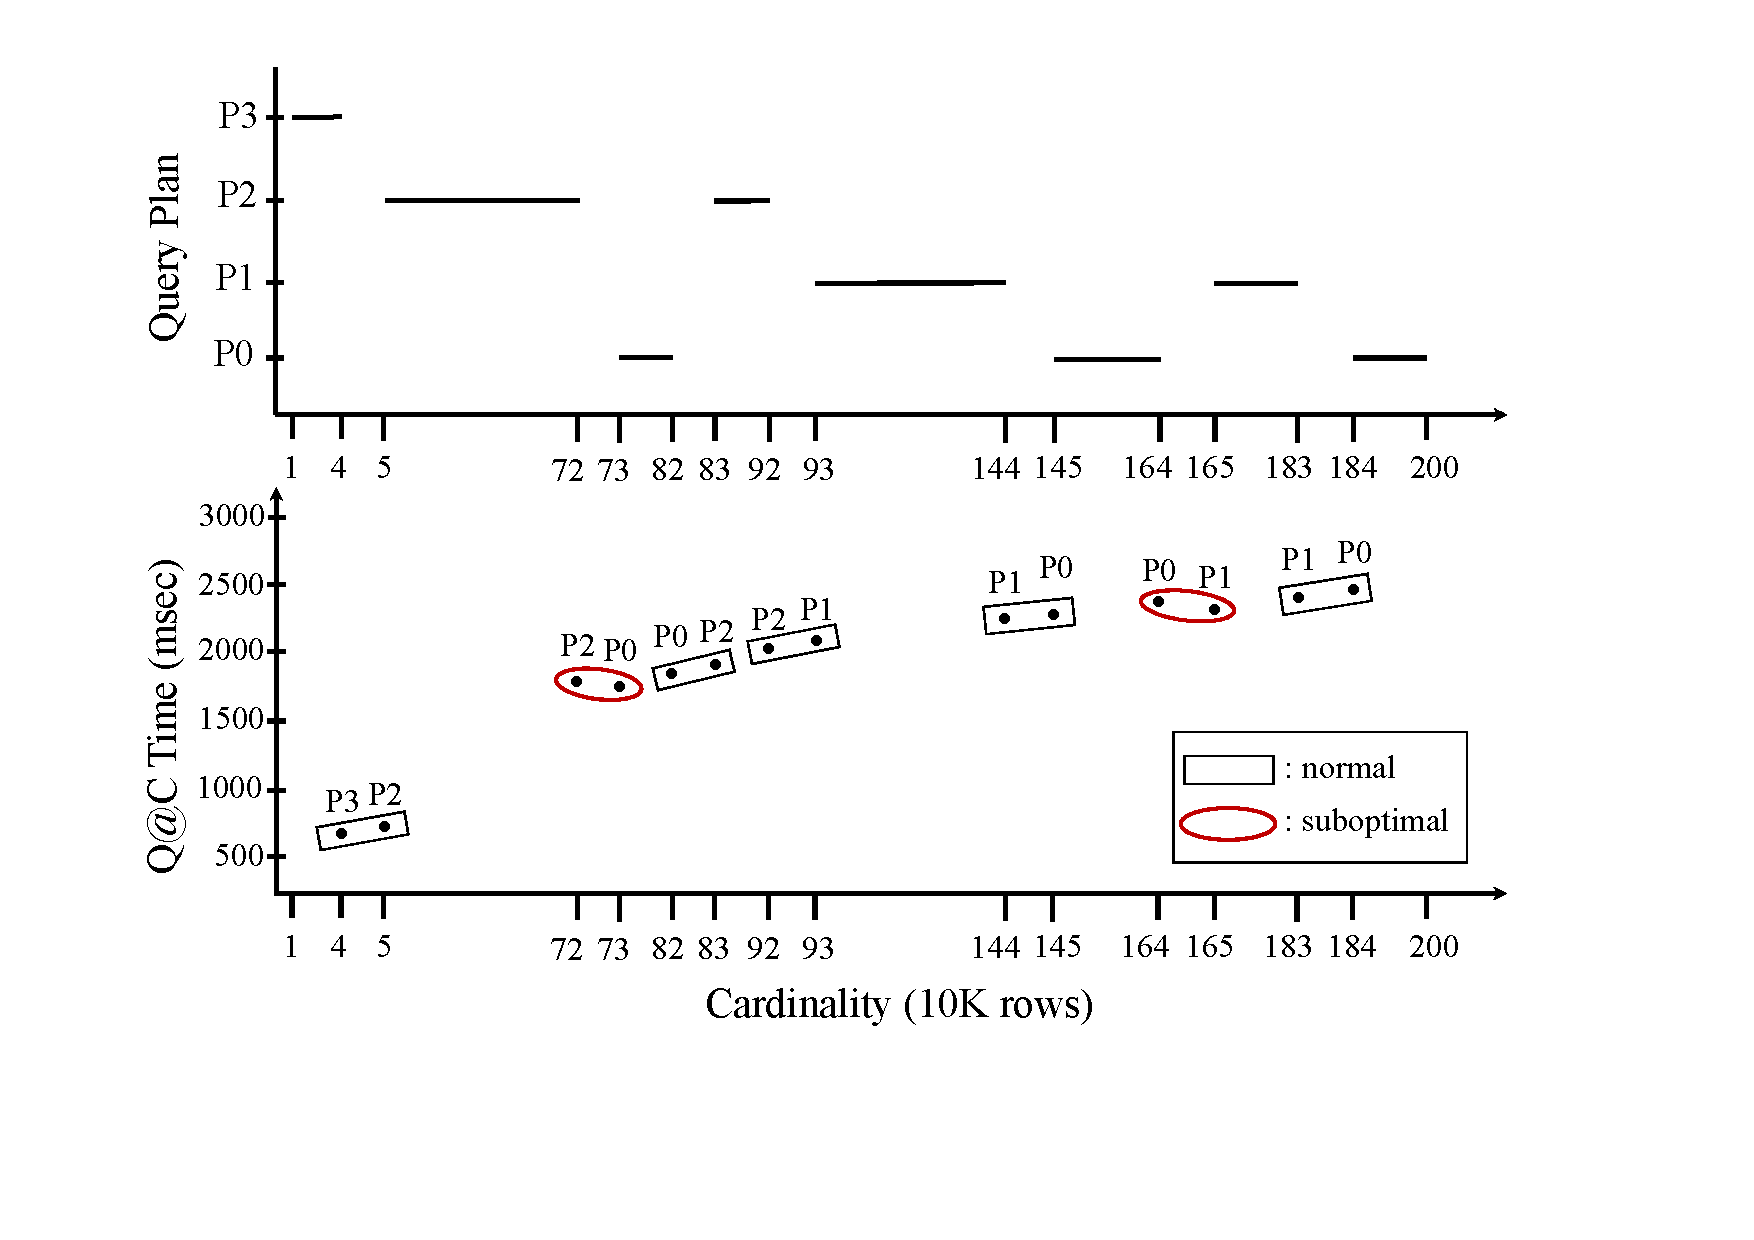
\includegraphics[width=30pc]{figures/subopt_flutter.pdf}
%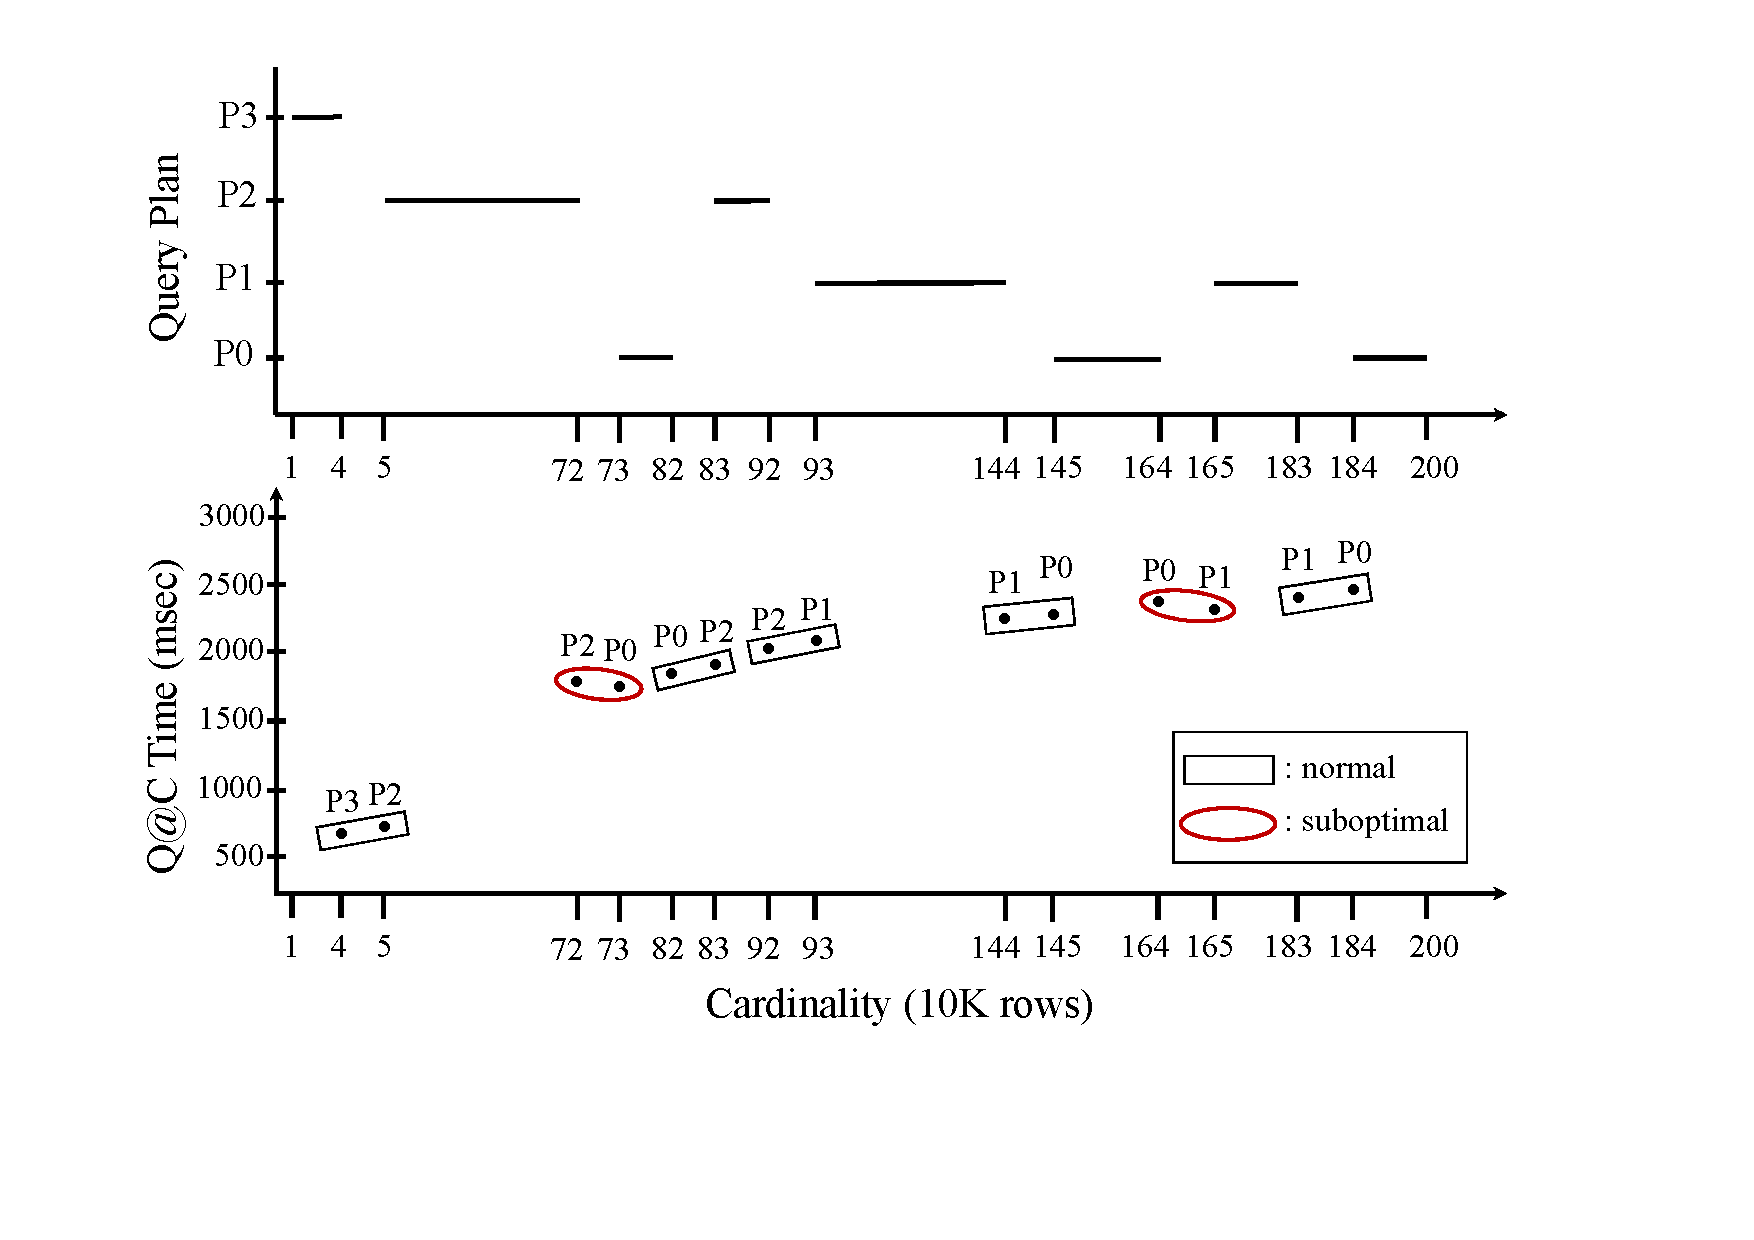
\includegraphics[scale=0.42]{figures/subopt_flutter.pdf}
\caption{An Example of Suboptimality and Fluttering\label{fig:query769}}
\end{figure*}

The lower graph in Figure~\ref{fig:query769} indicates the query times
executed at adjacent cardinalities, termed the
``query-at-cardinality'' (Q@C) time, when the plan changed. For some transitions, the Q@C time at
the larger cardinality was also larger, as expected. But for other
transitions, emphasized in red ovals, the Q@C time at the larger cardinality
was {\em smaller}, such as the transition from plan P1 at 1,650,000 to P0 at 1,640,000
tuples: the plan at the higher cardinality actually took {\em less} time
than the plan at the lower cardinality. Such {\em change pairs}, where the time at the
  higher cardinality is shorter, identify suboptimal plans. For the change pair at 720,000
tuples, P0 required 2.35sec whereas P1 at a larger cardinality required
2.41sec (as is common, the plan at the higher cardinality takes more time). This query exhibits seven plan change pairs, two of which are suboptimal.

This query also illustrates an interesting phenomenon, in which the
optimizer returns to an {\em earlier} plan. Sometimes the
optimizer starts oscillating between two plans, sometimes even switching
back and forth when the cardinality estimate changes by a small
percentage. The example query showed returning to P0 twice and to P1 and to
P2 each once.
We call this phenomenon, in which
the query optimizer returns to a previous plan,
``query optimizer flutter'', or simply ``flutter''.

We have found through our experiments that flutter and suboptimality are all
around us: {\em every} \hbox{DBMS} that we have examined, including two
open source \hbox{DBMSes} and two proprietary
\hbox{DBMSes}, covering much of the installed base worldwide, exhibit these
phenomena, even for very simple queries. In the Confirmatory
Experiment described in detail in Section~\ref{sec:experiments}, we started
with 6,967 query instances (a query run on a specific \hbox{DBMS}) after \doubleblind{our}{an} extensive query measurement
protocol~\cite{TTPv1,TTPv2} applied its extensive sanity checks. While about
20\%, or 1,491, of these query instances contained only one
plan, a few of the other query instances switched plans at almost every change in cardinality (we varied the
cardinality in increments of 10K tuples, a total of 200 cardinalities): see
Figure~\ref{fig:planchanges}. Slightly over half, or 3,933 query instances, exhibited
suboptimality somewhere along those 200 cardinalities; a few had
many changes to a plan that was in fact suboptimal, as indicated in
Figure~\ref{fig:suboptplanchanges}, across all four \hbox{DBMSes} considered.

\begin{figure}[t]\centering
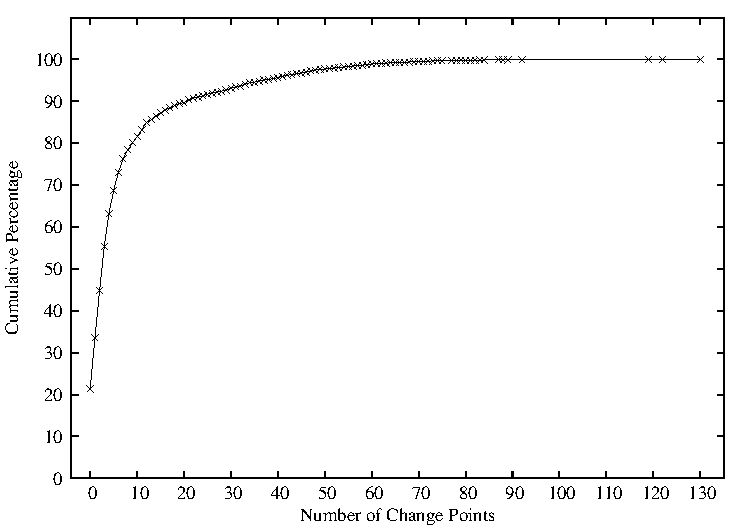
\includegraphics[width=0.60\textwidth]{figures/org_ncpq.pdf}
\caption{Cumulative percentage of queries \hbox{exhibiting} the \hbox{indicated}
  number of plan changes\label{fig:planchanges}}
\end{figure}

\begin{figure}[t]\centering
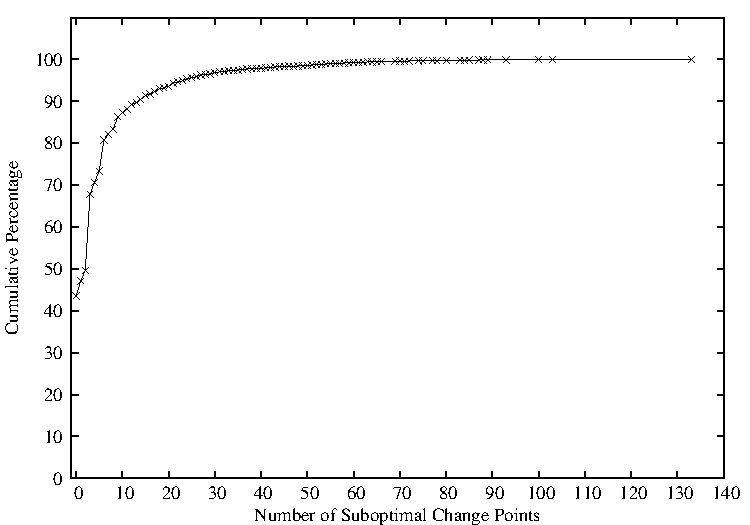
\includegraphics[width=0.60\textwidth]{figures/zi_ncpq.pdf}
\caption{Cumulative percentage of queries exhibiting the \hbox{indicated}
  number of changes to a {\em suboptimal} plan\label{fig:suboptplanchanges}}
\vspace*{-2ex}
\end{figure}

One oft-stated observation is that the role of query optimization is not to
get the {\em best} plan, but rather to get a plan that is acceptably
good. (Thus, the very term ``query optimizer'' is aspirational rather than
accurate.) Figure~\ref{fig:suboptcumulative} shows
the cumulative distribution of the relative amount of suboptimality (where
an $x$-value of 100 denotes that the query ran 100\% slower than the optimal
query, that is, twice as long). The good news is that 2,738 query instances,
or 67\% of the suboptimal queries, exhibited only a small degree of
suboptimality: less than 30\%. The challenge is that over fifth of all
queries (1,355) exhibited a significant amount of suboptimality ($\geq
30\%$). The relative slowdown can thus be quite large for some queries.

We started with 7,640 query instances, each of which is a particular query running on a
particular DBMS, cf.~Experiment 7 of Table~\ref{tab:run_stat}
in Section~\ref{sec:experiments}. After our protocol, we were left with
  6,967 query instances, of which 5,475 had at least one change pair, so those are
  the ones we consider further. Of those, 1,382 had {\em no} suboptimality, so
4,093 (75\%) had some suboptimality. 

1,951 (36\% of the query instances with a change pair) have the higher cardinality
running at least 20\% faster than the lower cardinality. That means that
2,142 query instances (slightly over half of the suboptimal queries) were barely
suboptimal ($<$20\% slower) and about a third (1,355) were considerably
suboptimal (where the higher cardinality ran at least 30\% faster than the
lower cardinality).

\begin{figure}\centering
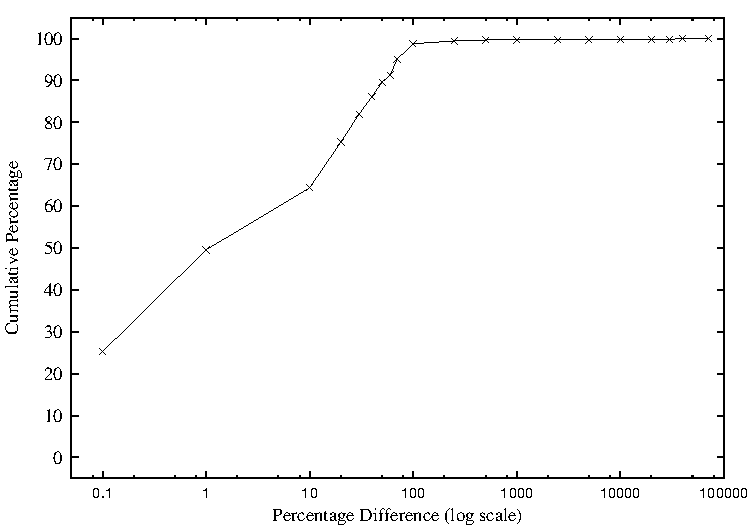
\includegraphics[width=0.60\textwidth]{figures/rel_diff.pdf}
\caption{Cumulative percentage of queries exhibiting the \hbox{indicated}
  percentage relative suboptimality\label{fig:suboptcumulative}}
\end{figure}

We emphasize four important points.
\begin{itemize}
\item First, we used a sophisticated query
measurement methodology that reduces the measurement variance, so that the
query plans we identify as suboptimal definitely are so.
\item Second, these
results are over four \hbox{DBMSes}, and thus, such phenomena are not dependent on
a particular implementation of cost-based optimization. Rather, they seem to
be common to {\em any} cost-based optimizer, independent of the specific
cardinality \hbox{estimation} or plan costing or plan enumeration algorithm or
implementation.
\item Third, suboptimal plans are {\em not} the result of poor
coding or of inadequate algorithms. We view query optimization in modern
\hbox{DBMSes} as an engineering marvel, especially given the complexity of the SQL
language and the requirements and expectations of \hbox{DBMS} users, who often
demand that important queries simply not get slower with a new release of
the \hbox{DBMS}. Rather, the prevalence of suboptimality observed here is a
reflection of the complexity of the task of query optimization.
\item Fourth, we wanted to understand whether a fundamental
limitation exists in the prevalent approach to query optimization utilized
by DBMSes generally, and certainly by the four DBMSes that we studies.
\end{itemize}

This is why we needed a new methodology. We want to understand cost-based
optimization deeply. This means that we need to go beyond the examination of
a single query optimizer, as is done in almost every paper (with a few
important exceptions~\cite{harish07,Haritsa10,Leis15}) over the forty-year history of
query optimization research, to study multiple instances of that
optimization architecture, in an effort to achieve generalizable results.

Thus, in this paper, we articulate a predictive causal model for how and in
what circumstances suboptimality arises and provide compelling evidence via
\hbox{hypothesis} testing that this model accurately characterizes the
\hbox{behavior} of query optimizers in general. This is what is meant by
``empirical generalization''~\cite{cohenbook} and why it is needed to answer
such questions. In the long history of research in database query
optimization, or even of databases in general, our model and its hypothesis
tests are the first predictive results that we are aware of that apply {\em
  across} \hbox{DBMSes}, rather than on a single, specific \hbox{DBMS} or on
a specific algorithm. Our goal is to make statements
that hold across cost-based optimizers in general, thereby moving up the
$y$-axis of Figure~\ref{fig:empirical}.
Such a DBMS-agnostic, though paradigmatic, causal
model can then \hbox{provide} guidance to the community about where fundamental
research is needed and to the \hbox{DBMS} engineers about where to focus
their efforts.

\begin{figure*}[t]
\centering
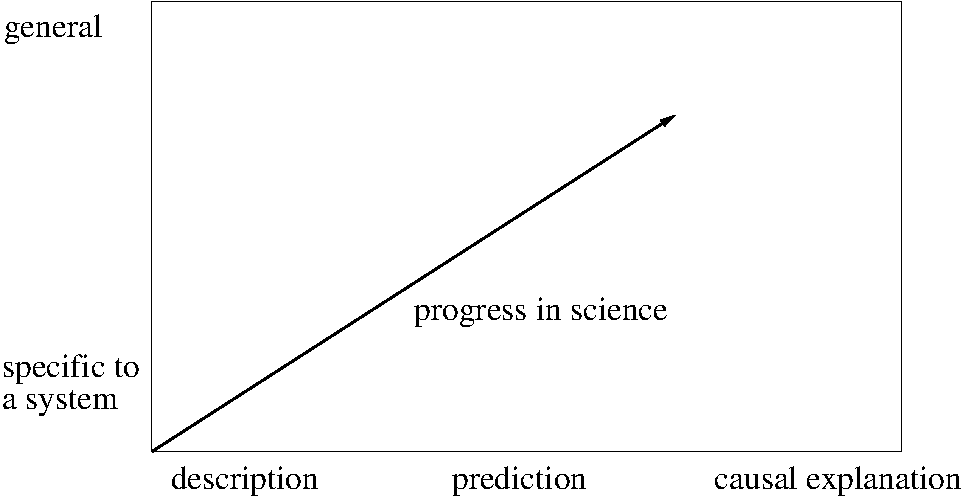
\includegraphics[width=0.60\textwidth]{figures/understanding.pdf}%0.40
\caption{Empirical Generalization\label{fig:empirical}}
\end{figure*}

\section{Related Work}\label{sec:related}

\shorten{SQL has emerged as the {\em de facto} and {\em de jure} standard relational
database query and update language. It emerged as an ANSI and ISO standard
in 1986--7, with a major extension and refinement as SQL-92~\cite{Melton93} 
and an even larger extension as SQL:1999~\cite{Melton03} and refinement as
SQL:2008~\cite{SQL2008} and SQL:2011~\cite{Melton11}.  
}
There has been extensive work in query optimization over the last 40
years~\cite{Ioannidis96,Jarke84}, during which a particular quite effective
paradigm had taken hold, in both open-source and proprietary DBMSes. In this
over-arching paradigm, query optimization and evaluation
proceeds in several general steps~\cite{Ramakrishnan03}. First, the SQL query is 
translated into alternative query evaluation plans based on the 
relational algebra via {\em query enumeration}. The cost
of each plan is then estimated and the plan with the lowest estimated cost
is chosen. These steps comprise query optimization, specifically {\em
cost-based query optimization}~\cite{Selinger}. The selected query plan is
then evaluated by the query execution engine which implements a set of
physical operators, often several for each logical operator such as
join~\cite{Graefe93}.

An influential survey~\cite{Chaudhuri98} identifies
the major themes that have pursued in the hundreds of articles
published on this general topic. Chaudhuri reviews the many techniques and
approaches that have been developed to represent the query plans, to
enumerate equivalent query plans, to handle some of the more complex lexical
constructs of SQL, to statistically summarize the base data, and to compute the
cost of evaluation plans. He also mentions some of the theoretical work
(which is much less prevalent) to understand the computational complexity of
these algorithms. Most of this research may be classified as adopting an
engineering perspective: how can we architect a query optimizer ``where 
(1)~the search space includes plans that have {\em low cost} (2)~the costing
technique is {\em accurate} (3)~the enumeration algorithm is {\em
  efficient}. Each of these three tasks is nontrivial and that is why
building a good optimizer is an enormous undertaking.'' \cite[page~35]{Chaudhuri98}


To determine the best query access plan, the cost model estimates the
execution time of each plan. There is a vibrant literature on this
\hbox{subject~\cite{Ioannidis03,Mannino88}}, including proposals for
histograms, sampling, and parametric methods. Again, most of these papers
are engineering studies, providing new techniques that improve on the
state-of-the-art through increased accuracy or performance. There have also
been a few mathematical results, such as ``the task of estimating distinct
values is {\em provably} error prone, i.e., for any estimation scheme, there
exists a database where the error is significant''~\cite{Chaudhuri98}.

An optimizer for a language like SQL must contend with a huge search space of
complex queries. Its first objective must be {\em correctness}: that the
resulting query evaluation plan produce the correct result for the
query. This objective must be ensured both by the initial SQL-to-relational
algebra translator and by the subsequent query enumerator. A secondary but clearly very important objective is {\em efficiency}; after
all, that is the raison d'\^etre for this phase. As is well known and has been
alluded to already, the name
for this phase is an exaggeration, as existing optimizers do not produce
provably optimal plans. That said, the
query optimizers of prominent \hbox{DBMSes} generally do a superb job of producing
the best query evaluation plan for most queries. This performance is the
result of a fruitful collaboration between the research community and
developers.

Early investigation of plan suboptimality resulted in approaches such as
dynamic query-reoptimization~\cite{Avnur,Bellamkonda13,kabra98,Li07}, which exploit more
accurate runtime statistics that appear while a query is being executed, to
steer in-flight plan reoptimization. The very presence of such a radical
change to the normal optimize-execute sequence indicates that plan
suboptimality was of interest to some researchers.

However, even with great effort over decades, optimizers as a general class
are still poorly understood. As has been observed, ``query optimization has
acquired the dubious reputation of being something of a black
art''~\cite{Babcock05}. DeWitt has gone farther, stating that ``query
optimizers [do] a terrible job of producing reliable, good plans [for
  complex queries] without a lot of hand
tuning''~\cite[page~59]{winslett02}. And as we will see, suboptimality may
occur in sophisticated query optimizers even when considering only simple queries.

While this paper does not provide direct solutions to address
suboptimality, we envision that by following up on the implications of our proposed predictive model
for suboptimality, engineering practice, such as dynamic reoptimization just
mentioned, may benefit. We elaborate on this subject in
Sections~\ref{sec:root} and \ref{sec:engineering}, where we discuss the engineering implications
of our causal model.

\section{A Model of Suboptimality}\label{sec:model}

The purpose of query optimization is to generate optimal plans.  So
why would suboptimality occur in the first place? Query optimizers are
highly complex, comprised of tens or hundreds of thousands of lines of code. There
are several reasons for this complexity. First, an optimizer must
contend with the richness of the SQL language, whose definition
requires about 2000 pages~\cite{SQL2008}, with a multiple of
linguistic features. Second, an optimizer must contend with the
\hbox{richness} of the physical operators available to it. \hbox{DBMSes} have a
range of algorithms available to evaluate each of many algebraic
operators. Third, the optimizer must contend with an exponential
number of query evaluation plans. Kabra and DeWitt~\cite{kabra98}
identify several other sources of complexity: inaccurate statistics on
the underlying tables and insufficient information about the runtime
system: ``amount of available resources (especially memory), the load
on the system, and the values of host language
variables.''~(page~106). They also mention user-defined data types,
methods, and operators allowed by the newer object-relational
systems~\cite{Melton03}. Thus, the task of optimization is very
complex, with the result that the optimizers themselves consist of a
collection of ``components'', that is, the rules or heuristics that it
uses during optimization, with each of these components being itself
complex.

We wish to understand the causal factors of suboptimality, through a
predictive model that explicitly states the relationships between these
causal factors. We test this model through experiments over tens\shorten{14,700} of thousand
of queries and hundreds of thousands of query executions\shorten{2.4M}, showing that there
is strong support for this model. We then extract engineering implications
from the model, suggestions for the most productive places to look to reduce
suboptimality and thus to improve existing query optimizers.

\begin{figure*}[tb]
\centering
%originally 30pc
%\epsfig{figure=figures/model.pdf,width=30pc}
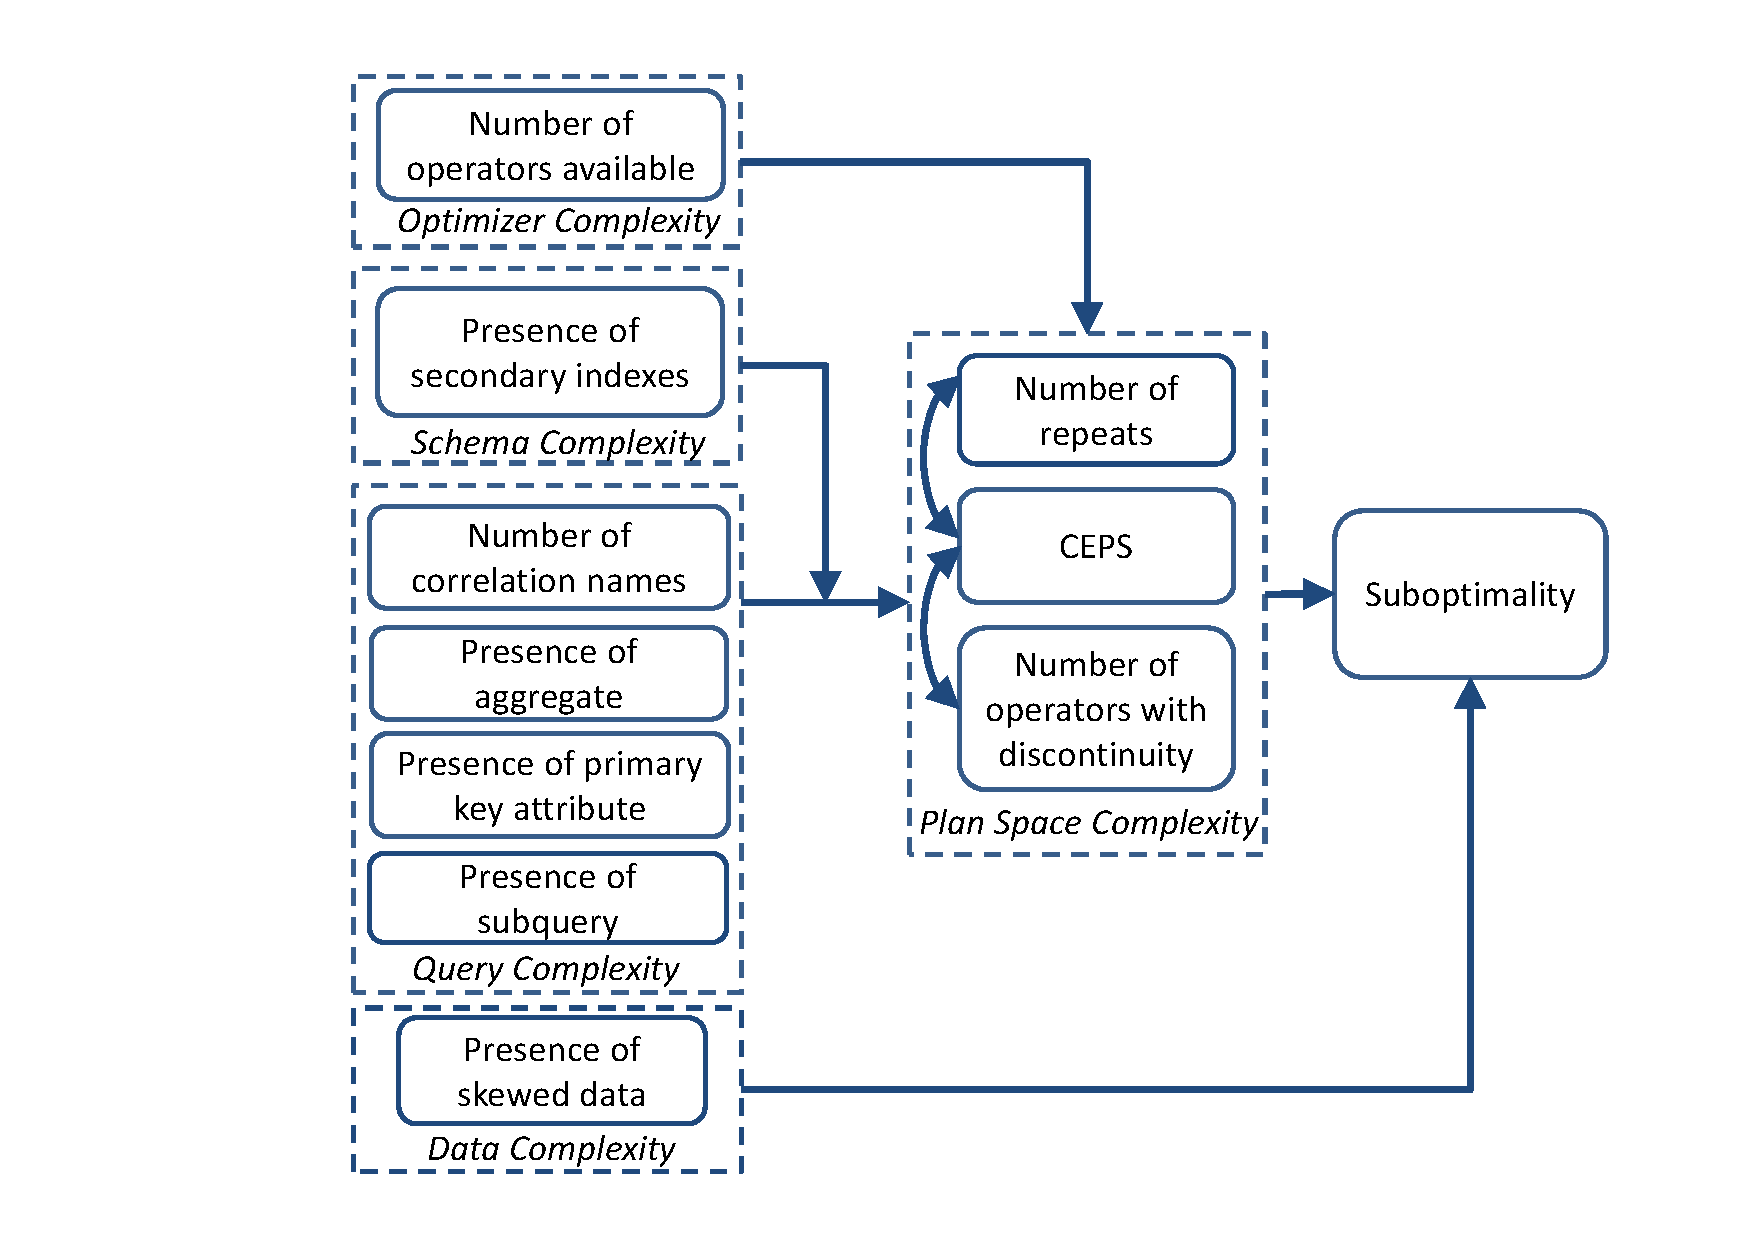
\includegraphics[width=30pc]{\discont{figures/subopt_model.pdf}{figures/subopt_model_wo_disc_op.pdf}}
\caption{Predictive Model of Suboptimality\label{fig:model}}
\vspace*{3ex}
\end{figure*}

Here we examine the hypothesized influence that each independent
variable will have on the one dependent variable, query Suboptimality (with
some of the influences mediated by one of the constructs). In
the next section we will operationalize these variables, explaining how
each is controlled or measured.

\subsection{Constructs in the Model}

The model concerns five general
constructs that we \hbox{hypothesize} will play a role in suboptimality: optimizer
complexity, schema complexity, query complexity, data complexity, and plan space complexity.
Two constructs include several specific variables that contribute to that
construct as a whole. Our model distills many of the widely-held assumptions
about query optimization. Our contribution is the specific \hbox{structure} of
the model and the specific operationalization of the
\hbox{factors} included in the model.

Our theory, which we will investigate in some detail and which is the
basis for our predictive model, is that suboptimality is due in part
to the complexity of the optimizer and concomitant 
interactions between the different components used within the 
optimizer with various sources of complexity in producing a good (hopefully
optimal) plan.  We argue that with the proliferation of concerns and
variability that an optimizer must contend with, it is extremely
difficult to ensure that for an arbitrary query that the optimizer
will {\em always} pick the right plan. There are many sources of complexity
that may challenge one or more components of the optimizer; our theory
implicates specific sources as contributing to observed
suboptimal plans.

The model depicted in Figure~\ref{fig:model} suggests specific factors that may
impact the prevalence of suboptimality. This model has one dependent
variable, {\em Suboptimality} (as noted in Section~\ref{sec:intro}, specifically, {\em empirical query suboptimality}), on the far right. We observe this \hbox{dependent
}variable in our experiments by determining whether each particular query,
run on a particular \hbox{DBMS} and using a particular schema,
is suboptimal at any cardinality of the input table. In Section~\ref{sec:operationalization}, we
delve into the details of how we operationalize this and the other variables
we now examine. The last two sections summarize our contributions and
suggest three fundamental directions that are suggested by this study.

\subsection{Variables in the Model}
The model has several independent
variables which influence Suboptimality.

For the construct of {\em optimizer
complexity} we have one independent variable, ``\hbox{Number} of operators
available (in the \hbox{DBMS})''. We can manipulate this variable by our choice of
\hbox{DBMS}: each \hbox{DBMS} has a set of operators available to its query
evaluator and available to the query optimizer to use with in query plans.

We have one variable for the construct of {\em schema complexity}:
``Presence of secondary indexes''. If true, that means that every
non-primary-key attribute, for the table for which we vary the cardinality
(termed the {\em variable table}) as well as for the other three tables
(termed the {\em fixed
tables}), has a secondary index associated with it. The rationale is that the
Presence of secondary indexes expands the number of possible plans: each
predicate in the query can often be mapped to one or more operators
utilizing that index.

For the construct of {\em query complexity} we have identified four
variables: ``Number of correlation names'', ``Presence of aggregate'',
``Presence of primary key attribute'', and ``Presence of subquery''. For each independent
variable, we have interventional control in our experiments, in that we can
manipulate the values of these variables through the construction of the
actual query to be optimized. The first is the number of correlation names
defined in the FROM clauses. The second is whether a single aggregate operator
({\tt Sum}) appears in the SELECT clause. The third
is whether a primary key attribute appears in at least one predicate in the
WHERE clause. The fourth is whether a single subquery appears in the
WHERE clause; that subquery evaluates to a single value that is
equality-compared with an attribute, in the where clause. The rationale is
that each factor may expand the number of plans or otherwise render the search for
the optimal plan more complex.

We have one variable for the construct of {\em data complexity}: that of
``Presence of skewed data''.  Skew is generally defined as how values are
distributed with a column of a table. We refine this to ``how many duplicate
values are present,'' with zero skew meaning that there are no duplicate
values present and 100\% skew implies that there is but one value in the
entire column. The Presence of skew complicates query time estimation, which
in turn complicates the search for the optimal plan.

In the middle of the figure is the construct of {\em plan space
complexity}. Given a particular query, its
complexity will impact the total number of candidate plans considered
by the optimizer. This variable is not directly
observable, again, especially for proprietary \hbox{systems}. However, we {\em
can} measure the number of plans actually generated by the optimizer
when presented with different cardinalities of the underlying tables.
We term this set of plans the ``effective plan
space'' and term the number of such plans, the cardinality of the
effective plan space, or ``{\em CEPS}''. Similarly, \discont{we cannot directly observe
the cost model utilized by the optimizer for the operators it considers, but
can classify the cost model of each operator as continuous (smoothly varying
with cardinality of its input(s) and without jumps) or discontinuous
(sometimes producing observable jumps in the predicted
cost), and can thus count the ``Number of operators with
discontinuity''. (Such operators have also been termed
``nonlinear''~\cite{Hulgen03}, though we focus on a more specific aspect of
discontinuity.) Finally,}{} the variable ``Number of repeats'' {\em is}
directly measurable as the number
of times a plan is reused across the cardinality of the variable table. (We
discussed plan reuse and the related phenomenon of {\em flutter} in
Section~\ref{sec:motivation}; Figure~\ref{fig:query769} provided a concrete
example in which plan P0 was encountered three separate times across the 200
cardinalities.) For
example, if the sequence of plans for a query as the cardinality increases
is $A ~ B ~ B ~ B ~ C ~ C ~ A ~ B ~ B~ B ~ C ~ B ~ C ~ C ~ C ~ B$, then the
``Number of repeats'' will be six: removing sequential duplicates results in $A ~ B ~ C
~ A ~ B ~ C ~ B ~ C ~ B$, with the last six distinct plans being duplicates
of the first three. Note that CEPS plus the number of repeats gives you the
number of plans in the sequence, again, after removing sequential
duplicates, nine plans in this particular case. Thus, we associate with the latent construct
of plan space complexity \discont{three}{two} measurable (that is, indirect) variables. Our
  model stipulates that the construct, and thus the \discont{three}{two} associated with
  this construct, intervene between the constructs of optimizer complexity,
  schema complexity and query complexity and the construct of Suboptimality.

Plan space complexity is an {\em intervening} construct, in that it is dependent
on some of the constructs on its left but is observable and thus exerts influence on the dependent
variable on its right. We can observe these variables within experiments and
indirectly influence their value but
cannot directly intervene to specify their value. For example, we can influence the CEPS through
manipulating the values for the independent variables of optimizer and query
complexity, but cannot directly set a value for CEPS within an
experiment.

\subsection{Hypotheses in the Model}\label{sec:hypotheses}
Given these six constructs and \discont{eleven}{ten} specific variables depicted in
Figure~\ref{fig:model}, let's now examine the causal relationships between
these variables, each depicted as a directed arrow between variables (a line
originating or ending at a construct is interpreted as originating or ending at all
variables in that construct). The causal model predicts specific hypotheses  between
the the constructs (in particular, between their associated variables).

One causal factor of this model is the optimizer complexity. We hypothesize
that optimizer complexity has influence over suboptimality indirectly, via
plan space complexity. We hypothesize that an optimizer with a larger number
of available operators will generate more plans and hence increase plan
space complexity.

\vspace{0.6em}\noindent
{\bf Hypothesis 1}: Number of operators available will be positively
correlated with (a)~Number of repeats\discont{, (b)~CEPS, and (c)~Number of operators with
  discontinuity}{ and (b)~CEPS}.

\vspace{0.6em}We now turn to query complexity, a construct associated with four
independent variables. As with the optimizer complexity construct, we
include in our model an
indirect effect through plan space complexity.

A higher value of each of these specific variables implies a more complex
query.  We expect a strong relationship between Number of correlation names
to CEPS (because it is well-known that the number of potential join
combinations is exponential to the number of correlation names)\discont{,}{ and} to Number of
repeats (Number of repeats could partially track CEPS)\discont{, and Number of
operators with discontinuity (for the same reason)}{}.

We also expect a positive relationship between Presence of aggregate (as
that will definitely add at least one operator to the query plan), Presence
of primary key attribute, and
Presence of subquery.

\vspace{0.6em}\noindent
{\bf Hypothesis 2}: Number of correlation names will be
strongly correlated with (a)~Number of repeats\discont{,}{ and} (b)~CEPS\discont{, and (c)~Number of
operators with discontinuity}{}. Presence of aggregate will be positively
correlated those those \discont{three}{two} variables (correlations \discont{d--f}{c--d}) and similarly
with Presence of primary key attribute
(correlations \discont{g--i}{e--f}) and Presence of subquery (correlations \discont{j--l}{g--h}).

\vspace{0.6em}
We feel that skewed data (in the ``data complexity''
construct) will not impact plan space complexity. Rather, our expectation is
that it will negatively impact accuracy of plan cost estimation, and thus
increase suboptimality directly.

\vspace{0.6em}\noindent
{\bf Hypothesis 3}: Presence of skewed data will be negatively correlated with Suboptimality.

\vspace{0.6em}
Let's now turn to the plan space complexity construct. We hypothesize a positive
correlation between the two variables associated with this construct. As the
Number of plans considered by the optimizer increases, so should CEPS\discont{, which
could increase the Number of operators with discontinuity that is observed}.

The model also predicts \discont{two correlations}{a correlation} within plan space
complexity, between 
CEPS and \discont{Number of operators with discontinuity variables and with
}Number of repeats. \discont{

We hypothesize that greater plan space complexity should make it more
difficult to optimize the query.  It is important to note that the
occurrences of suboptimality is not necessarily dependent on the Presence
of an operator with discontinuity. However, we predict that when
discontinuous plan operators appear in candidate plans, they may introduce
complexity to query optimization, especially at the cardinality where
discontinuity is possible. This is because the performance of such operators
is sensitive to the input size in a rather complex way. Any inaccuracy in
the estimation of plan statistics may lead the optimizer to select a suboptimal
plan.

Similarly, a}{A} plan chosen by the optimizer once will be reconsidered at a
later cardinality and perhaps chosen, following
the past experience of selecting and using that plan among many other plans.
Even if many different plans are already used, 
for the same reason the optimizer may revisit a pool of 
the previously used plans and choose one of them than to explore other new plans, 
given the complexity of plan cost estimation. 
Then the larger CEPS, the more times the optimizer repeats using the same plans. 
We thus hypothesize that the Number of repeats has a positive correlation with CEPS. 

\vspace{0.6em}\noindent
{\bf Hypothesis 4}: Plan space complexity (CEPS) and \discont{(a)~Number of operators
with discontinuity and (b) }Number of repeats will be positively correlated.

\vspace{0.6em}
The schema complexity construct consists of the variable ``Presence of
secondary indexes''. Such indexes provide opportunities for the optimizer to
consider more candidate plans that use these indexes, due to the additional
query evaluation operators now applicable. Those additional plans enable the optimizer to
possibly do a better job, while also adding complexity to the optimization
process.  The quality of query optimization ``very much depends on how much
the query engine relies on [cardinality] estimates and on how complex the
physical database design is, i.e., the number of indexes
available.''~\cite{Leis15}.

We hypothesize that this factor has a more complex role in the
model, serving as a {\em moderator} of two relationships introduced
above. We hypothesize that the overall effect of the secondary indexes 
is to increase the strength of the relationship between query
complexity and to plan space complexity. (Note that as the Presence of primary
key is required for secondary indexes, we don't include that former
independent variable here.)

\vspace{0.6em}\noindent
{\bf Hypothesis 5}: Presence of secondary indexes will strengthen
the correlations between the Query Complexity construct, specifically, the
variables Number of
correlation names, Presence of aggregate, and Presence of subquery, and
the Plan Space Complexity construct, specifically, variables Number of
repeats\discont{,}{ and} CEPS\discont{, and Number
of operators with discontinuity (correlations a--f and \todo{Rick: check:}j--l listed above in
Hypothesis 2).}{ (correlations a--f listed above in Hypothesis 2).}

\vspace{0.6em}
Finally, we hypothesize that queries with a high plan space complexity
present challenges to the query optimizer, and thus increase the chance that
the query optimizer picks a suboptimal plan. \discont{This is a fairly direct
connection for CEPS and Number of operators with
discontinuity. For}{Specifically, for} the
Number of repeats variable, a query exhibiting a high number of repeats has
more opportunities for suboptimality at some cardinality, just because the
number of repeats is an indication that the query optimizer is struggling.

\vspace{0.6em}\noindent
{\bf Hypothesis 6}: Suboptimality will be positively correlated with Plan
space complexity, that is, (a)~Number of repeats\discont{, (b)~CEPS, and (c)~Number
of operators with discontinuity}{ and (b)~CEPS}.

\vspace{0.6em}
We have just {\em described} how
suboptimality might arise, through a theory and its elaborated causal model,
which implies six specific hypotheses (some with multiple components).
We now need to move to {\em prediction}.
How might we test such a model? 

The first step to test this model is to {\em operationalize} each
variable. In the next section we describe explicitly how each variable is
defined. For the independent variables, we must be able to intervene, that is,
set their values before the experimental test commences. For the
dependent variables, we need to be able to measure their values during each experiment.

\section{Variable Operationalization}\label{sec:operationalization}

In this section we specify how we operationalized each of the seven independent
variables in the model.  Recall that each independent variable is a property
of a \hbox{DBMS} (Number of operators available), of the schema (Presence
  of secondary indexes), of a query (Number of correlation names,
Presence of aggregate, Presence of primary key attribute, and
Presence of subquery), of the data (Presence of skewed data), and of
the plan space (Number of repeats\discont{, CEPS, and Number of operators
  with discontinuity}{ and CEPS}). There is 
one dependent variable of our model (Suboptimality).

It is important to note that manipulation must be done {\em
  outside} the \hbox{DBMS}, as we do not have access to the
internal code of proprietary DBMSes. Hence, we do not know ({\em cannot} know) all the plans that were
considered, nor the details of how the plans were selected. But such access
is not needed; indeed, to be able to study a phenomenon across many \hbox{DBMSes},
such access is not feasible. But by designing the experiment to examine
the plans that each \hbox{DBMS} actually produces, and thus to examine phenomena
that can be externally visible, we can obtain valuable insights into general
classes of computational artifacts. 

\subsection{Optimizer Complexity}
By ``Number of operators available'' we mean the \hbox{number} of operators
available in the \hbox{DBMS} for selection, projection, join and aggregate
functions (that is, potentially relevant for our queries). Our
experiments intervene on this variable by selecting a particular \hbox{DBMS} on
which to evaluate each query. Across the available \hbox{DBMSes}, as the Number of
operators available increases, the complexity of the optimizer increases
because it has to choose between more operators.

The {\tt EXPLAIN PLAN} facility specifies the operators(s) \hbox{employed} in that
plan. For each \hbox{DBMS}, we collect the unique operators from the plans
and count the number of these distinct operators, each used by for at least one
query at at least one cardinality by that \hbox{DBMS}. The Number of operators used
by a \hbox{DBMS} ranged from 8 to 53 across the queries and data sets
used in the Exhaustive, Exhaustive with Keys, and Exploratory Experiments,
to be discussed in Section~\ref{sec:experiments}.

\subsection{Schema Complexity}
Presence of secondary indexes is easy to operationalize. We generate two
databases, one without any secondary indexes and one with a key specified
for each table on the non-key (that is, other than the first) attribute.

\subsection{Query Complexity}\label{sec:querycomplexity}
Query complexity is also relatively easy to operationalize. We randomly generate queries,
such as the example presented in Section~\ref{sec:motivation}. Each query
is a select-project-join-aggregate query, with a few attributes in the
SELECT clause, a few tables \hbox{referenced} in the FROM clause, a few
equality predicates in the WHERE clause, and zero or one aggregate
functions in the SELECT clause. As such, some of the complexities
mentioned by Kabra and \hbox{DeWitt~\cite{kabra98},} such as
user-defined data types, methods, and operators, are not
considered. Concerning Presence of primary key attribute, if this independent
variable was set to 1, we ensured that there was at least one primary key
attribute in one of the comparisons in the WHERE condition.

The queries were generated
by a simple algorithm\shorten{, the pseudo-code for which is shown in
Figure~\ref{alg:querygen}}. 
\shorten{The query generator has four main components, which are {\tt
  generateSelectClause()}, {\tt generateFromClause()}, {\tt
  generateWhereClause()}, {\tt generateGroupByClause()}. , and {\tt buildAggregateStatement()}.}
The SELECT clause will contain from one to four
attributes, hence, an average of 2.5 attributes. The Number of
correlation names
in the FROM clause varied from one to four, with duplication of tables
allowed (duplicate table names within a FROM clause implies a self-join).
In the queries that were generated, from one to four tables were
mentioned in the FROM clause. Somewhat fewer tables were mentioned than the
Number of correlation names, as the Presence of self-joins reduces the
number of unique tables referenced by the queries.

For the query in Section~\ref{sec:motivation}, the Number of correlation
names is 3, the Presence of aggregate
is false (0), the Presence of primary key attribute is false (0),
and the Presence of subquery is false (0).

%\pagebreak
\shorten{In {\tt generateWhereClause()}, in which all the joins will appear,
  we}We ensure that Cartesian products are
eliminated\c2j{.}{\shorten{({\tt cartesianPossible="false"})}.}  We do this by
connecting the correlation names that appear in the FROM statement via
equi-joins on random attributes. The comparisons are all
equality operators. To ensure that the queries are as simple as possible, we
do not include any additional predicates in the WHERE clause.  \c2j{}{This
  is realized by setting the attributes {\tt maxIsAbsolute} to {\tt true}
  and {\tt complexUsePercentage} to {\tt 100}.  Basically, ``complex''
  predicates eliminate the Cartesian product, and by setting complex
  predicates as ``absolute'', no additional predicates are included except
  for those which are necessary for eliminating Cartesian product.} Also
for simplicity, we include neither disjunctions nor negations.

\shorten{In the \todo{Correct name: generateGroupByClause}, where the aggregate
functions and
grouping occurs, the presence or absence of a group by clause is
recorded. We expect the
complexity of the query to increase when the first aggregate function
is introduced. (We don't consider in this model whether
additional aggregate functions in the same SELECT clause add
complexity}

The value of Presence of subquery was 0 or 1, with 0 indicating no
subquery. For each query needing a subquery, we picked a separate generated query and
rendered it as a subquery to replace an attribute in the WHERE clause of the
original generated query. The following query is an example where this
variable had a value of 1.

\begin{verbatim}
SELECT t0.id2, SUM(t1.id3)
FROM ft_HT2 t0, ft_HT2 t1
WHERE (t0.id2=t1.id1)
GROUP BY t0.id2
\end{verbatim}

We then generated another simple select-project (SP) 
query at random concerning the variable table 
and simply replaced one side (in this case, the right side) with the generated entire 
query as a subquery, to produce this final query.

\begin{verbatim}
SELECT t0.id2, SUM(t1.id3)
FROM ft_HT2 t0, ft_HT2 t1
WHERE (t0.id2 IN (SELECT t2.id3 FROM ft_HT1 t2)) 
GROUP BY t0.id2
\end{verbatim}
We thus have a maximum of only one level of nesting.

\subsection{Data Complexity}\label{sec:datacomplexity}
This independent construct has one variable: Presence of skewed data.

Skew has a very specific definition in statistics, 
involving elongating the left or right tail of a distribution, 
thereby moving the mean left or right of the median 
(in a symmetric distribution the mean = median = mode).

But we start with a distribution without a tail: 
the uniform distribution: the values from 1 to 2 million (2M). 
We consider this to be a skew of 0 (no skew). 
At the other end of the spectrum is one in which all the values are identical, 
or a skew of 1.0.

We define the skew as ``the reciprocal of the Number of distinct
values,'' so $0 < \hbox{\em skew} \leq 1$.
For 2M distinct values, the skew would be $\nicefrac{1}{2M}= 0.000005$, which is practically 0. 
For exactly one distinct value, the skew would be 1.0. For two distinct values, 
the skew would be 0.5. For ten distinct values, the skew would be 0.1.

We can generate the table of 2M rows by generating values sequentially from
1 to the Number of distinct values.  This creates a ``span of values.'' We
repeat this for the second span if necessary, and on and on, until we have
2M values in all.

When varying the cardinality, we remove 10K values from the variable table
and then copy those tuples to a new table to ensure that every page is as
full as possible (that is, 100\% load factor).  This gives us a table of
1.99M tuples. (We then get a query plan for this table.)  We repeat this
removal process until the final cardinality reaches 10K.

The way we effect the 10K removal is as follows. 
The key idea is to remove individual spans until we've deleted 10K
values. Since we don't touch the remaining spans, the Number of distinct
values does not change, and so the skew remains constant.

We use two values of skew: $\nicefrac{1}{2M}$ (termed {\em tiny}) and
$\nicefrac{1}{10K}$ (termed {\em small}).
\shorten{Let's first illustrate with a skew factor of 1.0. 
This translates to exactly 1 value for the entire table, or 2M spans.
To shorten, we remove 10K spans, equal to 10K values. 
This removal keeps the skew at 1.0, due to the unique values in the
remaining spans.
At the end, 10K spans, each with a single value, remain.

What about a skew factor of 0.1? 
This skew factor translates to 10 distinct values. 
So we generate 200K spans, each with ten values. 
To shorten, we delete 1,000 spans, which is equivalent to removing 10K values. 
As before, this does not change the skew.
At the end, the table will have 1,000 spans with 10K values, retaining a
skew factor of 0.1.

At the other end of the spectrum, consider a skew factor of
1/2M.  This skew factor, which is almost 0, gets translated to 2M
distinct values.  So}For the former, we generate a single span of 2M values.  To shorten the
table, it makes no sense to remove this single span in its entirety. But we
can remove 10K values from this single span.  Note that this changes the
skew to 1/1.99M, then eventually to 1/10K, which is still very close to zero
(the skew has changed from .0000005 to .00001).
For the latter, we generate 2,000 spans each of 10K tuples, and drop a span
to reduce to 1.99M tuples, repeating.
\shorten{We use five skewness values: 0.000005 (which we term only slightly
misleadingly as ``no skew''), 0.001, 0.1, 0.5, and 1.0,
for this independent variable.}

\subsection{Plan Space Complexity}\label{sec:discontinuity}

This explanatory construct includes \discont{three}{two} variables.

As discussed in Section~\ref{sec:model}, the ``cardinality of the effective plan
space'' (CEPS) is the number of plans selected as optimal for that query
being evaluated on one of the 200 cardinalities for the variable table. It
is ``effective'' because it was chosen, as opposed to the
plans that were considered but not chosen. (Recall that for proprietary
\hbox{DBMSes}, we do not have access to such plans.) Note that we count only
distinct plans. As we saw in Figure~\ref{fig:query769}, fluttering queries
return to a previous plan. This particular query has a CEPS of 4.

The Number of repeats is just the number of times a plan associated with a
smaller cardinality is repeated, after removing sequential
duplicates. 

\discont{We also wanted to evaluate the contribution of cost model non-linearity to
suboptimality. We found that it is possible to assemble, from outside the
\hbox{DBMS}, an approximation of the cost formula for that operator, and thus
directly observe whether it is non-linear. Specifically, the result of SQL's
{\tt EXPLAIN PLAN} (a result that is particular to each \hbox{DBMS}) includes the
{\em estimated cost} of each stage of the plan. That cost (estimate) is a
dependent variable, one that can be observed.

To operationalize the ``Number of operators with discontinuity'' we
classify each \hbox{DBMS} operator as either continuous or discontinuous, to be
defined shortly.  We then examine the queries
to identify the plan change pairs, which provide the {\em effective plan
  space}, a set of plans chosen for one or
more cardinalities of the variable table. For each distinct query plan in the
effective plan space, we
count the number of discontinuous plan operators that appear in that plan. Some of
these plans may contribute no such operators, some may contribute one such
operator, and some may contribute several such operators. We then sum the
counts of the distinct plans in the effective plan space, yielding an
integer as its operationalization
for each query.  This count per query varied from 0 to 85 for the
queries we tested in the confirmatory analysis.

To classify each operator as continuous or discontinuous, we use the data
from the ``Exhaustive'' experiments to be described in detail in Section~\ref{sec:experiments}. We
used a small subset of queries to be used later in testing the model, to
attempt to observe the same operators as encountered in that
study. We
collected the query plan at each possible cardinalities (200 in all) and
looked for ``jumps'', that is, when the cost model for an operator in the
plan exhibited discontinuity. Jumps are determined from the estimated cost
extracted from each plan operator. We provide an example of a jump below. If
a jump is observed, we classify that particular plan operator as
discontinuous.

A {\em jump} is a pair of close cardinalities (in our case, separated by 10K
tuples) in which the query optimizer's cost model is {\em discontinuous},
that is, does not smoothly increase from the lower cardinality to the upper
cardinality. To identify jumps in the first step, we examine the slopes
between each pair of adjacent cardinalities (again, separated by 10K
tuples). We expect that the slope (that is, the first derivative) is
well-behaved and thus does not change much for adjacent cardinalities. 
A jump thus indicates a large deviation in the second derivative of the 
cost model across the two cardinalities.

The Exhaustive experiments gather the cost model for each operator in each
plan for each cardinality (in our case, for cardinalities ranging from 10K
to 2M in steps of 10K, or 200 cardinalities in all that were examined).  Figure~\ref{fig:discontinuity}
presents for a single query\shorten{({\em query4}, exhaustive-10q-1,
  oracle)}, the {\em cost} of each of the hash-join operators utilized in
each plan at a particular cardinality. Each distinct point in the graph
depicts the computed cost of an individual hash-join operator over an input
table of the indicated cardinality (showing only a small portion of the 200
cardinalities).  This figure is typical
(we generally observed jumps at low cardinalities for these particular queries and
relation sizes).  As shown by this figure, the hash-join operator
represented by `+' has two discontinuous jumps, both appearing below
cardinality 150K. The other hash-join operator represented by $\times$ has one
discontinuous jump.  Between the jumps, the behavior is linear. It is our
guess that
such a jump is caused by the transition between one pass of a disk-based hashing
technique to two passes (and indeed for one of the operators, perhaps the one
lower in the operator tree, the transition to three passes, hence, the two
jumps). That said, all
that matters for our predictive model is that operators that experience
such discontinuity in their cost models present opportunities for
suboptimality.

%\begin{figure}[t]\centering
\begin{figure}[t]
\centering
%\includegraphics[width=0.70\textwidth]{figures/discontinuity_400K.pdf}%0.40
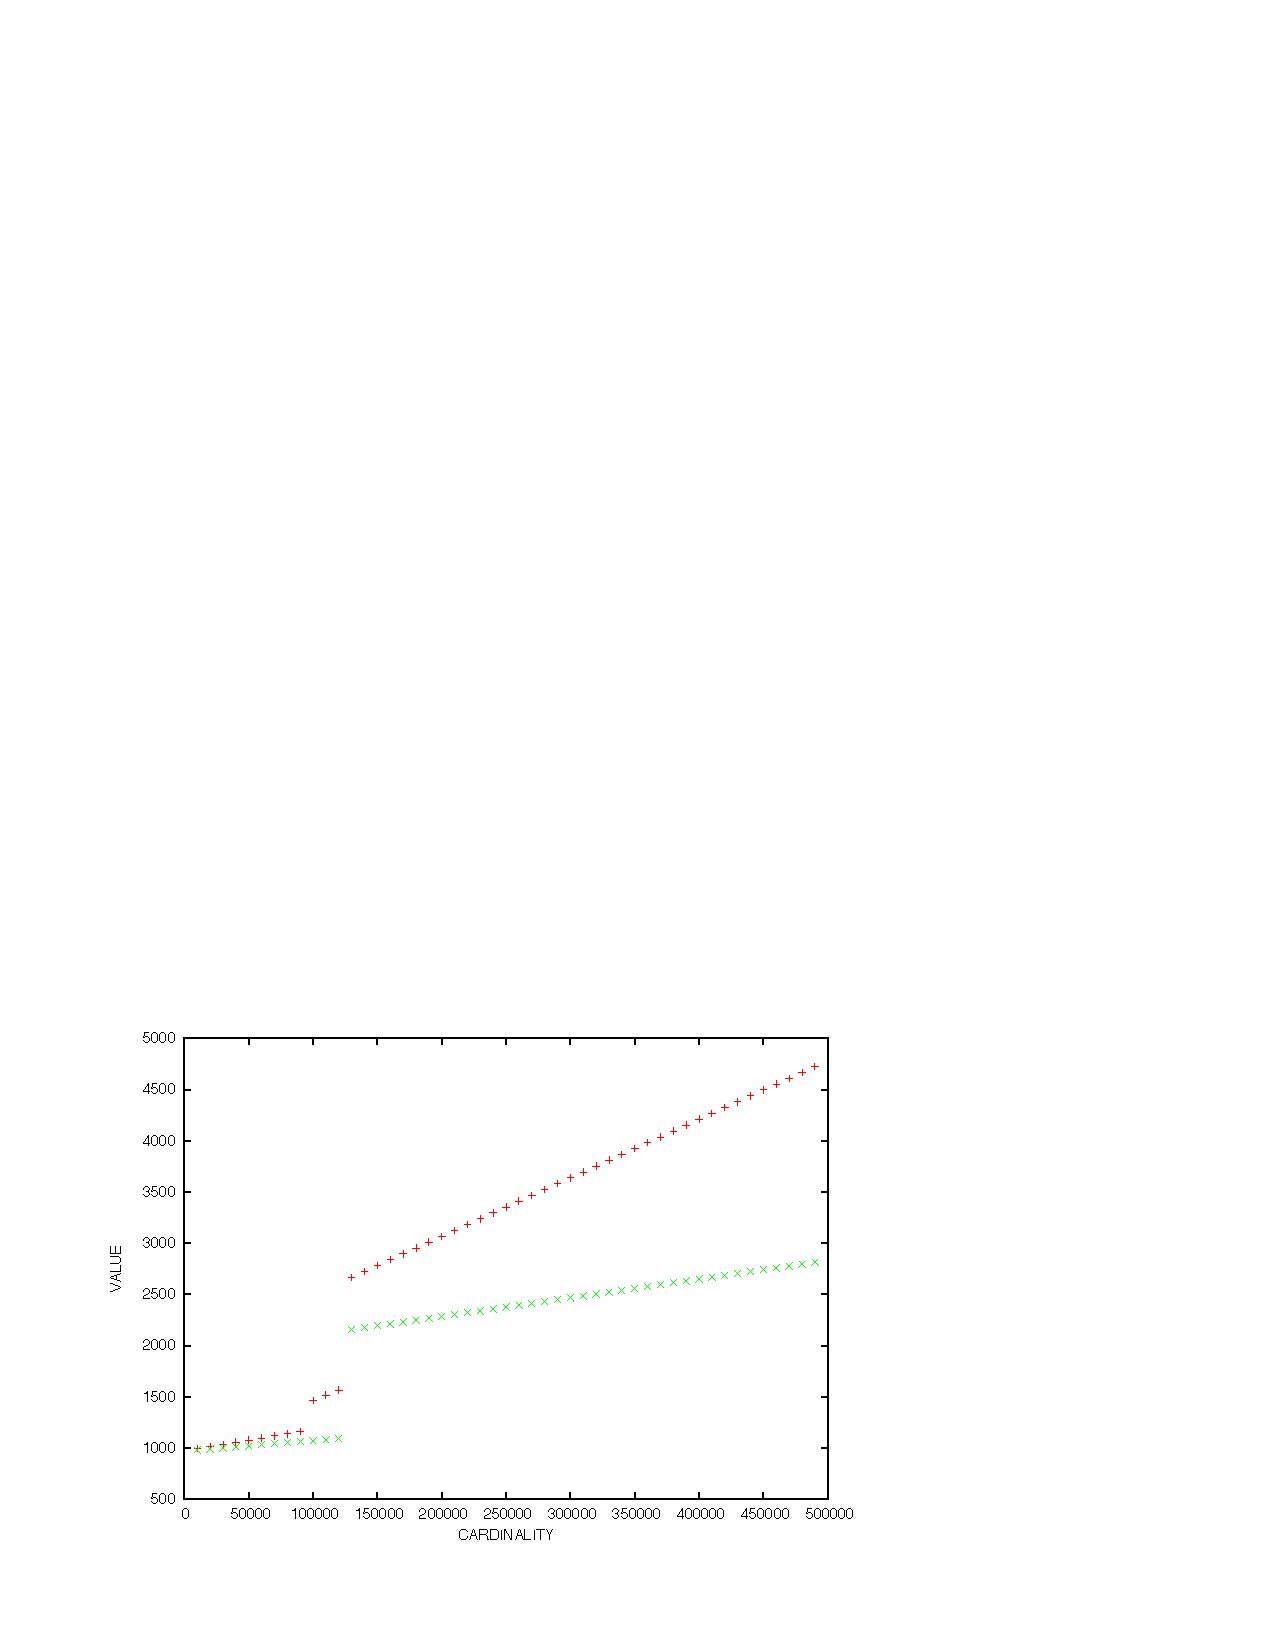
\includegraphics[width=0.60\textwidth]{figures/discontinuity_500K.pdf}%0.40
\caption{An Example of Discontinuous Plan \hbox{Operators (Hash-Join)}}
\label{fig:discontinuity}
\end{figure}

\shorten{It is interesting that jumps occurred only at smaller cardinalities. This
might depend on the strategy of how the \hbox{DBMS} utilizes the main memory
buffer.  Assume that the \hbox{DBMS} attempts to use as little memory as possible.
One possibility is that when the cardinality is low, memory allocation is
done in small chunks. Hence as the cardinality grows, more passes are
required. However, when tables get larger, bigger
chunks of memory would be allocated, requiring the operator to take longer
to fill up the available memory. We again emphasize that our focus is on predicting
suboptimality. Perhaps memory allocation has a role in operator
discontinuity, which our model predicts to have a role in query
suboptimality.
}
To identify such jumps, we examine the second derivative (the change in the
first derivative, that is, the change in the slope). A jump will be indicated by a larger than normal second
derivative. By identifying a sudden change in the second derivative, we can
effectively spot the cardinality at which an operator in a plan becomes
discontinuous.

Formally, we compute the slope ({\em S}) of the {\em estimated} cost
(of the cost model, formalized as $C_{\hbox{\small\em card}}$,
where {\em card} is the input
cardinality) between each pair of adjacent cardinalities as
$S_{\hbox{\small\em card}} = (C_{\hbox{\small\em card} + 10K} -
C_{\hbox{\small\em card}}) / 10K$~.
This computes a series of slope values.
We then compute the standard deviation of the slope
values.  For example, examining Figure~\ref{fig:discontinuity}, the slopes
are small except at three places, one for the green operator and two for the
red operator. By identifying the slope values that are greater than one
standard deviation over the average value, the discontinuous operators can
be identified: A ``discontinuous operator'' is one for which a jump is
observed in that operator in one of the plans for at least one of the input
queries.
}{}

\subsection{Empirical Suboptimality}\label{sec:suboptimality}
We now consider the one dependent variable at the core of this investigation.
How might suboptimality be observed? We have developed a system, \azdb, that
allows us to perform experiments to study this phenomenon of suboptimality.
\hbox{\azdb} submits queries to the \hbox{DBMS}, while varying
the cardinality of one of the tables,
requesting in each case the evaluation plan chosen by the \hbox{DBMS}.
This is done using the
{\tt EXPLAIN} SQL facility available in modern \hbox{DBMSes}. (The Picasso system
also used this facility to visualize the plan space chosen by a \hbox{DBMS}
optimizer~\cite{harish07,Haritsa10}.) We can then compare
the performance (execution time) of various plans for the query, to identify those
situations when a suboptimal plan was chosen, when in fact there was a
different plan that was semantically equivalent to the chosen plan (that is,
yielded the identical result) but which ran faster.

We modify the cardinality to produce multiple execution plans for a given
query. For one of the \hbox{DBMSes}, we can modify the stored table
statistics directly. For the other \hbox{DBMSes}, we had to do so
indirectly, by varying the size of the table and running the optimizer on
tables of different size. As we vary the cardinality, we collect the plans
that the optimizer felt were appropriate for that query at the various cardinalities.

Our definition of suboptimality assumes that
actual execution time for any query plan is {\em monotonically non-decreasing}, that is,
unchanged or increasing as the cardinality increases.  The intuitive justification is that at the higher
cardinality, the plan {\em has} to do more work, in terms of CPU time and/or
I/O time, to process the greater number of tuples.\discont{ (For an operator having a discontinuous cost model, as the
anticipated input cardinality grows, there will be {\em jumps}, in which the
predicted cost is temporarily much greater. Section~\ref{sec:discontinuity}
explains further how we specifically
operationalize this property. Also note that we don't consider SQL
operators such as {\tt EXCEPT} that are not monotonic.)}{}
We formalize this property as follows.

\vspace{1em}\noindent
{\bf Definition:} {\em Strict Monotonicity}: given a query $Q$ and an actual
cardinality $a$,

\quad\quad\quad\quad\quad$\forall p \in \hbox{\em plans} (p) \;\forall c > a \;( \hbox{\em time} (p,
c) \geq \hbox{\em time} (p,a) )$

\vspace{1em}\noindent
where {\em plans}($p$) is the set of plans generated by the optimizer and
{\em time}($p$, $c$) is the execution time of plan $p$ on the data set with
the varying table at cardinality $c$.\hfill$\blacksquare$

\vspace{1em}
\noindent
Note that the comparison is with the same plan $p$, occurring at higher
cardinalities.

To test this assumption, we ran an experiment that we term
``Monotonicity''. This experiment considered 60 queries, chosen from the
pool of queries
generated for testing suboptimality, and timed them for cardinalities from 10K
to 2M tuples, in steps of 10K tuples (hence, we used 200 cardinalities), for
each \hbox{DBMS} (for one \hbox{DBMS} that was very slow, we started with
30K tuples, as will be
discussed in Section~\ref{sec:experiments}). We varied the cardinality of the variable table by starting with
the maximum size, running the queries, then deleting 10K tuples and repeating.
We performed an ``{\tt ANALYZE TABLE}'' function to force
the \hbox{DBMS} to update the table's statistics to be accurate before actually
evaluating the query (we did this for all experiments).
We expected that as the cardinality decreased,
the run time would also monotonically decrease. However, due to the variance in query
time measurement observed even when the cardinality was identical, we encountered
spurious violations. 

Assuming a normal distribution for our time measurements, 95\% of 
the distribution falls within two $\sigma$ of the mean.
Therefore, to statistically
infer with a 95\% confidence interval that a violation occurred, 
we relaxed our definition of monotonicity to the following.

\vspace{1em}\noindent
{\bf Definition:} {\em Non-Strict Monotonicity}: given a query $Q$, an actual
cardinality $C$, and the standard deviation of the query executions for
cardinality C as $\sigma$, $Q$ is non-strict monotonic if $\forall p \in
\hbox{\em plans} (p) \;\forall c^{\prime} > C ((\hbox{\em time} (p, c^{\prime}) + \sigma_{c^{\prime}}) \geq
(\hbox{\em time} (p,C) - \sigma_{C}))~.~~\hfill\blacksquare$

\vspace{1em}
That said, the suspicious monotonicity violations raised the fundamental question of whether
we were using a sufficiently reliable timing method. The answer was {\em no}, as
the experiment used a (popular but) naive measurement technique 
based on \hbox{end-to-end} timing of which the results are 
typically perturbed by system noise potentially incurred during the measurement. 
We realized that the accuracy of this timing data was
insufficient for this monotonicity test.
We then switched to a new protocol, TTPv1~\cite{TTPv1}, and later TTPv2~\cite{TTPv2},
which fortunately is able to obtain quite accurate and precise timing.

Specifically, as we will see in Section~\ref{sec:experiments}, 
using the protocol we observed only 3,347 violations (0.74\%) of non-strict monotonicity, 
for the largest experiment (Experiment~7: Confirmatory) across all
the \hbox{DBMSes} we studied. 
Hence, this result justified our conclusion that the \hbox{DBMSes} under
study are indeed monotonic.

We can now turn to empirical suboptimality. Recall that the monotonicity test examines
two adjacent {\QatC}s for which the {\em same plan} is observed. To detect
suboptimality, we look for adjacent {\QatC}s with {\em different plans}, the
``change pairs'' mentioned earlier. We look for such change pairs where the computed
query time at the {\em upper} cardinality is {\em smaller} than the computed
query time at the {\em lower} cardinality. Say the lower cardinality used
Plan {\em A} and the upper cardinality exhibited Plan {\em B}. Had the \hbox{DBMS}
query optimizer selected Plan {\em B} for the lower cardinality, the query time would have been smaller than that for
Plan {\em A}, which follows directly from the
monotonicity assumption. The conclusion is that for the lower cardinality, the
optimizer picked the less efficient plan, and thus, this query exhibits
\hbox{suboptimality}. Note that since this approach cannot consider plans
that were never chosen, it very likely misses some suboptimal plans (for
which there was a better plan not seen), and thus produces a
conservative estimate of suboptimality.

Our definition of suboptimality compares the computed run times 
and standard deviations at the cardinality just before the change
pair (designated as $n-1$) and at the change pair (that is, $n$).

The query is said to be suboptimal if
%\hspace*{3em}
$\hbox{\em time}_{n-1} - 0.5 \cdot \hbox{\em stddev}_{n-1} \geq \hbox{\em
time}_n + 0.5 \cdot \hbox{\em stddev}_n$~.\\
In requiring at least one standard deviation of difference, versus just saying a Q@C pair is suboptimal if the time at higher cardinality is faster than the the time of plan at lower cardinality, we minimize spurious or minor differences in plan times. 
For each Q@C pair, Suboptimality is coded as four levels (0--3), based on the distance in 
standard deviations, up to three standard deviations. We chose this cutoff
because 99.7\% of Q@C pairs are less than or equal to three standard
deviations.
\shorten{\begin{itemize}
\item Not suboptimal, i.e., 0, when
$$\hbox{\em time}_{n-1} - 0.5 \cdot \hbox{\em
stddev}_{n-1} < \hbox{\em time}_n + 0.5 \cdot \hbox{\em stddev}_n $$
\item Low suboptimality, i.e., 1, when
$$\hbox{\em time}_{n-1} - 0.5 \cdot \hbox{\em
stddev}_{n-1} \geq \hbox{\em time}_n + 0.5 \cdot \hbox{\em stddev}_n$$
and
$$\hbox{\em time}_{n-1} 1 1.0 \cdot \hbox{\em stddev}_{n-1} < \hbox{\em time}_n +
1.0 \cdot \hbox{\em stddev}_n$$
\item Moderate suboptimality, i.e., 2, when
$$\hbox{\em time}_{n-1} - 1.0
\cdot \hbox{\em stddev}_{n-1} \geq \hbox{\em time}_n + 1.0 \cdot \hbox{\em
stddev}_n$$
and
$$\hbox{\em time}_{n-1} - 1.5 \cdot \hbox{\em stddev}_{n-1} < \hbox{\em time}_n +
1.5 \cdot \hbox{\em stddev}_n$$
\item High suboptimality, i.e., 3, when
$$\hbox{\em time}_{n-1} - 1.5
\cdot \hbox{\em stddev}_{n-1} \geq \hbox{\em time}_n + 1.5 \cdot\hbox{\em stddev}_n$$
\end{itemize}

\noindent}
We then sum this value over the Q@C pairs with different plans
(the change pairs) to arrive at a single integer for the query instance,
thus determining the {\em empirical suboptimality of that query instance}.

Note that while \azdb\ examines the plan at every cardinality, it only has
to actually execute the query at change
pairs.  Since many fewer {\QatC}s were involved, we could try many more
queries than the \hbox{Exhaustive} \hbox{Experiment}. In the Exploratory Experiment to be
described in Section~\ref{sec:experiments}, the value of Suboptimality ranged
from 0 (no suboptimality) to 133, with the majority between 0 and 9. A full 56\% of
the queries were suboptimal.  \hbox{Because} the occurrence of large values of this
measure was so rare, we did a log transformation: $\log_{10} (1 + \mbox{\em
  subopt})$ in the confirmatory analysis.

\section{Testing the Causal Model}
In this section we elaborate on how to test our model and discuss the test
results. Specifically, we describe in detail the environmental configurations,
data sets, and various experiments that we utilized. We then provide
descriptive statistics of the experiments and present the results of
correlational and regression analyses. 

\c2j{}{\subsection{Experimental Setup}\label{sec:setup}}
\shorten{As mentioned, we used \azdb\ to run the experiments. This infrastructure,
now comprising around 44K lines of code, handles all the details of
generating the sample data, generating the actual queries, collecting the
various plans generated by the optimizer, running the queries, and storing
the results in a ``labshelf'', a set of tables managed by
a separate \hbox{DBMS}. This infrastructure also performs the many steps
required to ensure repeatability.

We have assembled a hardware lab of dedicated
machines, one \c2j{for each DBMS}{each for the three \hbox{DBMSes}} and one to run the \hbox{DBMS} used
to store the lab shelves. Having dedicated hardware allows us to worry
less about other processes running on the machines that could dirty the
results (these machines are {\em only} for experiments), and allows us to
run extensive experiments involving days or weeks of computation. We have
used this software and hardware lab to perform a number of experiments
examining the phenomenon of suboptimality.
}
\shorten{{\azdb} utilizes experiments defined in XML. It supports {\em experimental
  scenarios}, which are short (perhaps 100 lines of code) Java subclasses
that provide details of how to run kinds of experiments.}

The measurements were collected using Tucson Timing
Protocol\linebreak Version~1 (TTPv1)~\cite{TTPv1} and Version~2 (TTPv2)~\cite{TTPv2} on a suite of five machines, each an
\hbox{Intel} Core i7-870 Lynnfield 2.93GHz quad-core processor on a LGA 1156 95W
motherboard with 4GB of DDR3 1333 dual-channel memory and Western Digital Caviar
Black 1TB 7200rpm SATA hard drive, running Red Hat \hbox{Enterprise} Linux
Server release 5.8 (Tikanga) for TTPv1 and release 6.4 (Santiago) for TTPv2, with a kernel of 2.6.32-358.18.1.  The protocol
provided calculated query evaluation time, including computation and I/O time,
in msec. Both protocols were utilized exactly as specified.

No run violated the experiment-wide sanity checks. For the largest
experiment, the Confirmatory Experiment (number 7) discussed below, approximately
10.5\% of the query executions (QEs) and 5.1\%
of the queries-at-cardinality (Q@Cs) were dropped due to query execution
and Q@C sanity checks. As a result, excessive variation in calculated query
time was observed in only 0.003\% of the Q@Cs. A total of 0.43\% of Q@C adjacent
pairs violated relaxed monotonicity and 0.74\% of the Q@Cs violated strict
monotonicity, which is acceptable.

\doubleblind{In fact, over the course of the research described here, we
  found that currently available techniques for measuring query time did not offer sufficient query time
  precision, and so we developed TTPv1~\cite{TTPv1} to provide that needed
  precision. As our research in suboptimality proceeded, we realized that
  to detect suboptimality for two adjacent cardinalities
  separated by only 10,000 rows (just a few database pages), or even in the case of
  MySQL, 300 rows, we needed even finer resolution. This provided the
  impetus for the massive effort to develop TTPv2~\cite{TTPv2}, which did
  indeed provide the needed precision.}{We
  thank the developers of this protocol and of the software that enabled the
  running of many, many queries for providing us this software.}

In these experiments, we  installed each disk directly
on the machine that also runs the DBMS, ensured a cold cache (disk drive,
disk controller, O/S, and DBMS buffer), and discarded any sequence of query
executions that appear to be the result of query result caching. We also
ensured within-run plan repeatability.

In the following, we describe in detail the data used by our experiments and
the experimental scenarios we defined. More details on both
can be found in Appendix~\ref{sec:app}.

\subsection{Data sets}\label{sec:datasets}
We generate our experiment data set randomly in each of the experiments. However, we
use seeds to control the random data generator so that it can produce
repeatable data as required.

Our experiment data set consists of relational tables. There are two types of
tables. The first is a ``fixed table'' that, once created and
populated, will never be modified in the future.  In contrast, the second
type is a ``variable table''. We alter the cardinality\c2j{ of
  this table}{, physically, of such tables} as the experiments are being performed. 
\c2j{We used a}{We generated four configurations for the data sets. The first configuration
is a small} data set with four tables, each with four integer-typed
attributes. The fixed tables were populated with one million rows and the
variable table with two million rows (sixty thousand rows for one DBMS). Thus, the size of the tables is roughly 16--32Mbytes, with tiny skew (cf.~Section~\ref{sec:datacomplexity}). We also produced versions of the data set
with (i)~small skew, (ii)~primary keys (of the first attribute), and (iii)~primary
keys and secondary indexes, for all tables, as detailed in Appendix~\ref{sec:appdatasets}.

\subsection{The Experiments}\label{sec:experiments}

We are interested in predicting the suboptimal behavior of \hbox{DBMSes} through our
model. We selected four relational
\hbox{DBMSes}, some open source and some proprietary, that are representative of
the relational \hbox{DBMS} market. Each was used in its stock configuration.

In each experiment, we varied the
cardinality from 2M (maximum) to 10K (minimum), in increments of 10K. For
the one \hbox{DBMS} that was slower than the others and was timing out for
the majority of the queries when run between 10K and 2M, we reduced the
size of the tables and varied the cardinality from 60K (maximum) to 300 
(minimum), in increments of 300.

Utilizing JDBC to manipulate independent variables from outside the
  \hbox{DBMS} allows us to empirically generalize by moving up the $y$ axis of
  Figure~\ref{fig:empirical}, from one system to several systems and then to
  a general theory. We don't reveal the identity of the \hbox{DBMSes} we studied, for two reasons. First, commercial \hbox{DBMSes}
include in their user agreements requirements not to release 
performance data. This is detrimental to science, but we have no choice but
to live with that restriction. However, in some sense the specific \hbox{DBMS}
doesn't matter, as we are studying phenomena about cost-based optimizers
{\em in general}, and so are interested in making statements that apply across
the experimental subjects in our study.

\begin{table}[t]
\tbl{Experiments 1--7: Detailed Run Statistics\label{tab:run_stat}}
{%
\resizebox{140mm}{!}
{
\begin{tabular}{c|c|c|c|c|c|c|c}
& {\em Experiment}& {\em Protocol} & {\em Cumulative} & {\em Number of}&{\em
    Number} &{\em Number}& {\em Number of}\\
& & & {\em Hours} & {\em Query Instances}&{\em of Q@Cs} &{\em of QEs}&{\em Retained QEs}\\
\hline
1 & Monotonicity 		& --- & 38 & 60 & 12,000 & 12,000 & 12,000\\
2 & Exhaustive		& TTPv1 & 1,672 & 160 & 32,000 & 320,000 & 244,787\\
3\shorten{4} & Exhaustive with Keys 	& --- & 28 & 200 & 40,000 & --- & ---\\
4\shorten{5} & Initial Exploratory 	& TTPv1 & 560 & 780 & 8,842 & 88,420 & 68,891\\%40512+26367+2012
5\shorten{3} & Refined Exhaustive 	& TTPv2 & 1,544 & 160 & 32,000 & 320,000 & 319,980\\
6 & Exploratory 		& TTPv2 & 1,663 & 1,200 & 12,560 & 125,600 & 114,377\\
7 & Confirmatory 		& TTPv2 & 11,375 & 7,640 & 99,558 & 995,580 & 890,631\\
\multicolumn{3}{c|}{\em Total}	& 16,880 & 10,200 & 236,960 & 1,861,600 & 1,650,666\\
\end{tabular}
}
}
\end{table}

We performed seven separate experiments, each looking at a different
aspect. \hbox{Table~\ref{tab:run_stat}} exhibits the statistics of running a number of 
queries in our experiments. All but the last column list the number of query
instances, etc., gathered by the protocol for each experiment. The last
column gives the number of query executions retained by the protocol. One of
the primary goals of TTPv2 was (i)~to reduce the number of query executions discarded due to
phantom processes that were indirectly detected and (ii)~to collect relevant measures 
directly associated with I/O, such as BlockIO Delay time~\cite{TTPv2}. 
Experiments 5, 6, and~7 benefited from that protocol. Other details about
the experiments can be found in Appendix~\ref{sec:otherdetails}.

The queries came from 16 query sets, summarized below with more details in
\hbox{Appendix~\ref{sec:querysets}}. It is important to emphasize that while the {\em queries} all came
from the same query pool and while the data sets were also shared by the
experiments (see the Appendix for details), the {\em query executions} for
the six experiments, except Experiment~3 with no timing and hence no QEs, 
are disjoint. As a side comment, we mention that for all four \hbox{DBMSes}, the query
plans generated by a \hbox{DBMS} for a particular \QatC\ of a particular query
varied between the experiments, but not between the QEs
of that Q@C, by virtue of the way \doubleblind{we designed the
measurement protocol}{the measurement protocol was designed}.

The first experiment, termed ``Monotonicity'', was described in
Section~\ref{sec:suboptimality}. This experiment ran quickly, as it
only involved 12,000 QEs. That experiment helped us realize that we needed
to be much more sophisticated in our approach to timing queries.

\doubleblind{After we developed our six-step TTPv1 protocol,}{When TTPv1
    became available,} we performed our
second experiment, termed \hbox{``Exhaustive'',} which more accurately tested the 
monotonicity assumption. 
This experiment involved 160 query instances, 32,000 \QatC s (thus the name:
we timed each query ten times at {\em all} cardinalities, generating 200
\QatC s for each query instance), and thus
320,000 QEs (ten QEs for each \QatC ), requiring 1,672 cumulative hours.  The (very small: 1.6\%)
percentage % (16312+8215)/(995321+587546) = 1.6%
of strict monotonicity violations observed was consistent with the remaining
variance of the query time measurement, concluding that none of
the \hbox{DBMSes} violated monotonicity. This also provides a validation of
our definition of suboptimality, which requires monotonicity.

\discont{We then used the plans generated from the Exhaustive Experiment to classify operators as
continuous or discontinuous, as discussed in detail in
Section~\ref{sec:discontinuity}. Again we note that this experiment used a subset of
the set of {\em queries} (but {\em not} query executions) from the query pool,
to ensure that we see the same operators as encountered in that
study.
}{}
We also ran an experiment (termed ``Exhaustive with Keys'') on the 
\hbox{Exhaustive} query set but using the data set with primary keys.\discont{ However, in this
case we did not actually execute
the queries (thus this third experiment was very fast), but rather just
examined the plans that were returned from the \hbox{DBMS} to identify
additional discontinuous operators (five more were found).}{}

The fourth experiment was an ``Initial Exploratory'' 
analysis of a prior version of the causal model.
That earlier model had fewer independent
variables yet also had more complex relationships. Specifically, the model
did not include the independent query complexity variables of Presence of
secondary indexes, Presence of subquery, nor the schema complexity
independent variable of Presence of secondary indexes, nor the plan space
complexity independent variable of Number of repeats. The prior model also
had Presence of primary key attribute in the schema complexity construct rather than
the query complexity construct. In reformulating that independent variable,
we were able to remove a complex mediating moderator between the plan
space complexity and suboptimality constructs.

%% The following shorten corresponds to TTPv1.
In the experiment we ran a representative sample of queries and data sets: (a)~600 queries of one
\hbox{DBMS}, (b)~120 queries of another \hbox{DBMS}, (c)~10 queries
from each other two \hbox{DBMSes}, all without primary keys defined, and (d)~10 queries
from each of the four \hbox{DBMSes} on the primary key data set, for exploration
across all combinations, a total of 780 query instances.  (Again, consult
Appendix~\ref{sec:querysets} for details on these query sets.)
We ran the \hbox{DBMSes} only on the
change pairs, unlike the Exhaustive experiments. The protocol retained about 78\% of the QEs. 

As a large number of QEs (roughly a quarter) were discarded by TTPv1 in
these experiments, and as these discarded QEs were correlated with query
time (and thus perhaps with suboptimality),
\doubleblind{we sought to develop a better measurement protocol, which was
  the impetus for TTPv2~\cite{TTPv2}}{we switched to a better measurement
  protocol that had recently become available: TTPv2~\cite{TTPv2}}.
%Our subsequent experiments indeed benefited from the improved protocol, producing 
%highly lossless ($\sim$5\% Q@C drop) but very clean ($\sim$1\% violation) data.
The fifth experiment then was to rerun the Exhaustive experiment  (we term this simply
``Refined Exhaustive'') using that protocol. The main purpose of this experiment 
was to reexamine monotonicity within in the enhanced
protocol.

We observed that the monotonicity violation rate decreased
from 1.54\% to 1.02\% for strict monotonicity and from 0.61\% to 0.60\% for
non-strict monotonicity, thereby reaffirming our monotonicity assumption
(the first benefit). Moreover, the number of retained QEs went up
significantly (compare 244K to 320K retained QEs, a second and the primary benefit of TTPv2), 
while the number of hours required actually went down somewhat (a third benefit).
These benefits reassured us of the quality of data 
for subsequent experiments via the improved protocol.\discont{ Incidentally, no new
discontinuous operators were identified in this experiment.}{}

%% The following corresponds to TTPv2.
We subsequently reran the exploratory analysis using TTPv2, this time on a larger sample of queries and data sets:
(a)~200 queries of four \hbox{DBMSes} without primary keys defined and
(b)~100 queries from each of the four \hbox{DBMSes} on the primary key data set,
for exploration across all combinations, a total of 1,200 query instances. % (= 300 $\times$ 4 (DBMSes))
We termed this sixth experiment ``Exploratory''. This experiment 
retained 12,100 {\QatC}s (3.7\% were dropped), concerning 1,123 query
instances (6.4\% were dropped). Only 443 strict monotonicity violations (0.78\%) and 301 relaxed
violation (0.54\%) were observed. This exploratory analysis allowed us to refine
the operationalizations.

The seventh and final experiment was used for confirmatory analysis of the model and thus was
called ``Confirmatory''. This was the most time-consuming of
the experiments. Here we
used (a)~800 queries on the data set without primary keys defined and (b)~510 of
those queries that had joins on the primary key attributes, on the data set
with primary keys, 
(c)~100 queries on the data set with tiny skew and primary keys,  
(d)~100 queries with a subquery on the data set without primary keys,  
(e)~100 queries on the data set with primary keys and secondary indexes defined, 
(f)~100 queries with a subquery on the data set with primary keys defined,  
(e)~100 queries with a subquery on the data set with primary keys and secondary indexes defined, and 
(g)~100 queries on the data set with primary keys and secondary indexes defined, 
for a total of 1,910 queries and a total of 7,640 query instances (over the
four \hbox{DBMSes}). (Again, see Appendix~\ref{sec:querysets} for details.)
We ran the \hbox{DBMSes} at the 99,558 {\QatC}s that were observed,
roughly 13 per query. The protocol accurately timed
both sides of adjacent {\QatC}s (53,547 change pairs in all).

In this Confirmatory Experiment, we observed 3,347 strict monotonicity
violations (0.74\%), and 1,966 relaxed monotonicity violations (0.43\%) (out
of a total of 452,684 Q@C pairs having identical plans and query instance), which provides
further confidence that monotonicity also applies to operators found in
queries over data in various contexts (as described above) and that our
operationalization of Suboptimality is a valid one.

In the remainder of this section, we focus using the measured independent
and dependent variables in the Confirmatory experiment
to test the predictions that arise out of our causal model in Figure~\ref{fig:model}.

\subsection{Descriptive Statistics}
Several initial conclusions can be drawn from this confirmatory experiment, which was the
culmination of several years of programming effort and about 30 months of
experimental runs, summarized in Table~\ref{tab:run_stat}. 

To illustrate the descriptive statistics with the Confirmatory
experiment, we started with 7,640 query instances. These
resulted in 99,558 Q@Cs, each with ten query executions (QEs). Some of these
QEs violated one or more of the (many) sanity checks specified within the
TTPv2 protocol, leaving a remaining 890,631
retained QEs. A few of the query instances then violated one or more of the
Q@C sanity checks in the protocols (657 in all), with 6,983 query instances retained. Additionally, 16 query instances were dropped {\em after} the
protocol because they were missing data for the only change pair in the
query.

We were then left with 6,967 queries, of which we make three general
observations. 
First, perhaps surprisingly, 
more than half (3,933 queries out of those that emerged) exhibited suboptimality
somewhere in the range of cardinality of the varying table. 
{\em Every} \hbox{DBMS} exhibits suboptimality.

Secondly, most (3,370) of those suboptimal queries (86\%) had the maximum value of
Suboptimality  (i.e., level 3) for at least one change pair.
\shorten{a big number for a query could be many pairs, each at a small
  distance, or a few pairs, each at level 3. How many queries had at least
  one pair with subopt>=3? Answer: 670 in 5.20, 36 in 5.3, 531 in 6.0. So,
  total of 1237; query used: select count(*) FROM (select distinct experimentid, experimentname, dbms, runid,
querynum from CF_Analysis_SuboptDefn_Ver1 where subopt>=3);
query used 7_10: select count(*) FROM (select distinct experimentid, experimentname, dbms, runid,
querynum from Cnfm_Analysis_SuboptDefn where subopt_sd>=3);}
The phenomenon of query suboptimality that we observed is likely to be a
fundamental aspect of either the 
\hbox{algorithm} (cost-based optimization) or the
creator of the algorithm (human information processing). Our model includes
both effects.

%\pagebreak
Third, concerning the causal factors of Suboptimality in our model,
\begin{itemize}
\item the cardinality of the effective plan space (CEPS) ranged from 1 to 24
plans across the cardinality range,
\discont{\item a total of 23 operators were classified as discontinuous, out of 26 in all,
\item the Number of operators with discontinuity observed in plans for a query
averaged 9.4, with 85 being the maximum,}{} and
\item the Number of repeats ranged from 0 to 108, with the mean being 4.99.
\end{itemize}
 
\subsection{Correlational Analysis}\label{sec:corr}
We tested Hypotheses 1--6 using the strength and significance of
correlations of variables involved. These hypotheses predict
\discont{21}{14} main effects
and \discont{9}{6} moderating effects. Table~\ref{tab:hyptest} lists the hypotheses
followed by the correlation observed when testing each hypothesis.  (``NS''
denotes not significant at the $p < 0.05$ level, the accepted standard for
significance. For each dependent variable, we used the Bonferroni correction
to control the familywise error rate. ``---'' denotes no prediction arising
from the model.)  As can be seen, most of the main effects (17) arising from
the causal model are supported and significant.  \discont{The four exceptions are
Hypotheses 1c, 2g, 2j, and 3, highlighted in italics in the table.}{The three exceptions are
Hypotheses 2e, 2g, and 3, highlighted in italics in the table.}

\begin{table}[t]
\tbl{Testing Hypotheses 1--7: Correlations on the Confirmatory Study\label{tab:hyptest}}{%
%\begin{center}
%\resizebox{150mm}{!}{
\begin{tabular}{c|c|c|c\discont{|c}{}}
{\em Variable}& {\em Suboptimality}&{\em Repeats}&{\em CEPS}\discont{ & {\em Discontinuity}}{}\\
\hline
\hline
Operators in \hbox{DBMS} & ---&  {\bf H1a:} 0.35 & {\bf H1b:} 0.27\discont{& {\bf
  H1c:} -{\em 0.09}}{}\\
\hline
Correlation names & --- & {\bf H2a:} 0.17 & {\bf H2b:} 0.46 \discont{&{\bf H2c:} 0.34}{}\\
\hline
Presence of aggregate & --- & \discont{{\bf H2d:} 0.04 & {\bf H2e:} 0.10 & {\bf H2f:} 0.29}{{\bf H2c:} 0.04 & {\bf H2d:} 0.10}\\
\hline
Presence of primary key attribute& --- & \discont{{\bf H2g:} {\em NS} & {\bf H2h:} 0.15 & {\bf H2i:} 0.14}{{\bf H2e:} {\em NS} & {\bf H2f:} 0.15}\\
\hline
Presence of subquery & --- & \discont{{\bf H2j:} {\em NS} & {\bf H2k:} 0.26 & {\bf H2l:} 0.20}{{\bf H2g:} {\em NS} & {\bf H2h:} 0.26}\\
\hline
Presence of skewed data & {\bf H3:} {\em -0.05} & --- & ---  \discont{& ---}{}\\
\hline
Number of repeats& {\bf H6a:} 0.62 & --- & ---  \discont{& ---}{}\\
\hline
CEPS &  {\bf H6b:} 0.61 & {\bf H4b:} 0.45 &  --- \discont{&{\bf H4a:} 0.72}{} \\
\discont{\hline
Number of operators with discontinuity & {\bf H6c:} 0.47 & --- & --- & ---\\}{}
\end{tabular}
}
%\end{center}
%}
\end{table}

\discont{Hypothesis 1c was not supported because the
correlation between Number of operators available and Number of operators
with discontinuity was negative, while we predicted positive
correlation. The strength of the negative correlation was small:
\hbox{-0.09}.

In looking into this further, we noticed that the number of operators deemed
discontinuous by our operationalization in Section~\ref{sec:discontinuity}
was quite high: 26 out of 29 operators in all. Note that the
operationalization utilizes the {\em estimated cost} of each instance of a
particular operator within an observed plan. (The reason is that we could
not directly measure {\em per-operator run times}: we were only able to measure
{\em per-plan run times}, that is, for each Q@C.) The estimated cost reported by
the DBMS sometimes exhibited a lower estimate for the same operator within the
exact same plan at a slightly higher cardinality, which is
counter-intuitive. These findings
indicated to us that perhaps our \hbox{operationalization} of ``discontinuous
operator'' incorrectly classified some operators, due to the vagaries in the
estimated operator costs, and thus this negative correlation is also in doubt.

Hypotheses ~2g and 2j, both involving Number of repeats, were not significant.}{}

Hypothesis 3 was
not supported because the correlation between Presence of skewed data (recall from
Section~\ref{sec:datacomplexity} that absence of skew is operationalized as
{\em tiny} skew and presence of skew is operationalized as {\em small} skew)
and Suboptimality was in the \hbox{opposite} direction. Specifically, we observed a negative correlation,
indicating that as the skew increases from tiny to small, Suboptimality
decreases, though only slightly:~\hbox{-0.05}.

In Table~\ref{tab:hyptest5}, we examine the interaction strength of
Hypothesis 5, between the Query Complexity and Plan Complexity constructs, when
the moderator (Presence of secondary indexes) has a value of absent (``Not
SI'') and when it has a value of present
(``SI''). As before, ``{\em NS}'' denotes no significant at the $p < 0.05$
level; three of these interactions become not significant when secondary
indexes are added. (Recall that it is not possible to compute the
interaction strength for Presence of primary key attribute in the presence
of secondary indexes.)


\begin{table}[t]
\tbl{Testing Hypothesis 5: Interaction Strength on the Confirmatory Study\label{tab:hyptest5}}{%
%\begin{center}
%\resizebox{85mm}{!}{
\begin{tabular}{c|c|c|c|c\discont{|c|c}{}}
{\em Variable}& \multicolumn{2}{|c|}{{\em Repeats}}&\multicolumn{2}{|c}{{\em CEPS}} \discont{& \multicolumn{2}{|c}{{\em Discontinuity}}}{}\\
%\hline
{\em }&{Not SI\em }&{SI\em }&{Not SI\em }&{SI\em }\discont{&{Not SI\em }&{SI\em }}{}\\
%&{\em }&{\em }&{\em }&{\em }\\
\hline
\hline
Correlation names & 0.17 & 0.15 &0.49 &0.39 \discont{& 0.36 & 0.27}{} \\
\hline
Presence of aggregate  & 0.04 & {\em NS} & 0.12 & {\em NS} \discont{& 0.31 & 0.22}{} \\
\hline
Presence of subquery  & 0.03 & {\em NS} & 0.18 & 0.17  \discont{& 0.14 & 0.13}{}\\
\end{tabular}
}
%\end{center}
%}
\end{table}

This table shows that the strength of all \discont{nine}{six} applicable and significant
interactions goes {\em down} just a little (on average by 0.04), which is
opposite to our prediction. Hence, this negative moderation seems small but
robust. One possibility is that rather than the added schema complexity of
indexes increasing suboptimality, secondary indexes may have {\em reduced} the complexity of query
optimization, since the role of secondary indexes within query optimization
is well understood, thereby reducing suboptimality.

In summary, most (\discont{19 out of 21}{12 out of 14}) of the main effect hypotheses were
significant at the $p < 0.05$ level. \discont{Two of those hypotheses were}{One of those hypotheses was} (weakly)
in the opposite direction. The hypothesized moderation (Hypothesis 5) of
Presence of secondary indexes was small but in the opposite direction. Thus,
most of the hypotheses in our model were strongly supported.

\subsection{Regression Analysis}\label{sec:regression}
One use of regression is as a further test of Hypothesis 5, which predicts a (positive)
moderation in the presence of query complexity, specifically the Number of
correlation names, Presence of aggregate, and Presence of subquery
independent variables. Thus our causal model predicts that the interaction
strength should increase when secondary indexes appear in the relational
schema. (The {\em direction} of moderation, whether positive or negative, is not involved in this test; rather,
an increase in interaction strength only supports that there is a moderating
effect, in either direction.) When
secondary indexes were not specified, our model explains 
7.23\% of the variance of Number of repeats\discont{,}{ and} 40.9\% of the variance of CEPS\discont{, and 35.7\% of the variance
of discontinuity}{}. When
secondary indexes were defined on the underlying tables, our model explains
7.23\% of the variance of Number of repeats\discont{,}{ and} 41.1\% of the variance of CEPS\discont{, and
38.9\% of the variance of discontinuity}. These findings are all consistent with our
hypothesis predicting a moderation effect of secondary indexes.

A second use of regression is to compute the amount of variance explained
for the intervening and dependent variables, to indicate how much of the
underlying phenomena are explained holistically by the model.
\shorten{We did regressions on the causal variables for CEPS, Number of repeats and for Number of
operators with discontinuity. Our model explained 41.1\% of the
variance for CEPS, 7.23\% of the variance for Number of repeats, and 38.9\% of the variance for
discontinuity. \shorten{need path analysis} 

} So we also ran a regression over the independent variables of the model that
predict suboptimality over the data from the Confirmatory experiment. 

Note that our experiment was over four highly complex DBMSes, each with
hundreds of thousands to millions of lines of source code, none shared.
Thus, one might expect the amount of variance explained to be low, with a
considerable amount of variance to be {\em within} the DBMS. What we are getting
at with our causal model is the impact of {\em shared} aspects that arise
from supporting (a)~a common data language (the relational model), (b)~a common
language (SQL), (c)~a common query evaluation approach (operators in the
relational algebra), and (d)~a common query rewriting approach (cost-based query
optimization). Given these basic commonalities, each DBMS supports a
certain number of operators, each is impacted by certain characteristics of
the schema, query, and data, and each generates a certain number of candidate
plans.

Our
model explained \discont{53.6\%}{52.2\%} of the variance of the Suboptimality dependent
variable. That means that over half of the variance of Suboptimality is
explained by our operationalizations of Optimizer Complexity, Schema
Complexity, Query Complexity, Data Complexity, and Plan Space Complexity.

To state this a different way, all other possible causes for Suboptimality
will in concert have less predictive power than the constructs and specific
variables included in the causal model introduced here.

And somewhat extraordinarily, it is the common aspects listed above that predict
Suboptimality, {\em not} the particulars embedded in the inordinate complexity of
each of these DBMSes.

\shorten{
In our experiments, we noticed that some of the \hbox{DBMSes} might at
different times pick a different plan for the same query at the same
cardinality. We addressed this in our experiment by running the optimizer
(with a JDBC {\tt PreparedStatement}) and then executing the query ten times
in fast succession. Each time we did an {\tt EXPLAIN PLAN}  to ensure that
the originally-chosen plan was indeed used (it was).

That said, at the next cardinality, the optimizer went into action again,
and so could have chosen a {\em different} plan for that new cardinality.
Our supposition is that such a {\em heuristic} optimizer introduces
some variance in the cardinality dependent variable.

To test this, we ran regressions on just the \hbox{DBMS} that was demonstrably {\em
  not} heuristic, for the common case of primary keys. Interestingly, only
the Presence of aggregate and CEPS were significant at the 0.05 level, yet
our model explains fully \% of the Suboptimality variance (and \% of the
CEPS variance and \% of the discontinuity variance). This might imply
that heuristic optimization itself introduces perhaps 10--20% of the variance.

The size of the regression coefficients also provides useful
information. From the regressions run on the data, for the
statistically significant causal factors, the highest coefficients, all in
predicting the Suboptimality dependent variable, were CEPS at , number
of tables involved at , number of discontinuous variables at ,
number of operators available in \hbox{DBMS} at . Note though that number of correlation
variables is highly correlated with CEPS; the regression will apportion the variance of the dependent
variable among these factors.
}

\subsection{Summary of Model Testing}
In our experimental design, we started with a structural causal model that
encapsulates our theory for how cost-based query optimizers might select a
suboptimal plan for a query at a cardinality. This model implies the six
specific hypotheses listed in Section~\ref{sec:model}. We then performed
a series of experiments,
\begin{itemize}
\item to refine our operationalizations: specifically \discont{discontinuity,
via the Exhaustive \hbox{Experiment}, and} Number of operators available, via the
Exhaustive with Keys \hbox{Experiment},
\item to test fundamental assumptions, specifically
monotonicity, via the Monotonicity and Refined Exhaustive \hbox{Experiments}, and
\item to test and make minor
refinements to our model: the Initial Exploratory and \hbox{Exploratory}
Experiments.
\end{itemize}
During this exploration, \doubleblind{once we completed the TTPv2 protocol,}{when the TTPv2 protocol became available,} we reran
\hbox{experiments} to avail ourselves of the increased precision due to a much
higher percentage of retained QEs and thus Q@Cs and query instances.

Throughout these six experiments, we were cognizant of the
possibility of Type 1 errors: false positives that lead one to believe a
relationship exists when it doesn't.
To control for such errors, we then performed the final Confirmatory 
Experiment on a completely different data set consisting of many more 
query instances, 7,640 in all, running on four \hbox{DBMSes} that each
utilize cost-based query optimization, to test
our refined model. Statistical inference is only possible in confirmatory
analysis, where the model and hypotheses are selected a priori.

Now that the causal model has been found to be supported by the confirmatory
\hbox{analysis}, we turn to possible implications of this model.

\subsection{Identifying Root Causes of Suboptimality}\label{sec:root}

Our goal in this paper has been to understand cost-based query optimizers
as a \hbox{\em general} class of computational artifacts and to articulate and test
a predictive model \hbox{characterizing} how such optimizers,
again, as a general class, behave.  This model can be used to further
improve \hbox{DBMSes} through engineering \hbox{efforts} that benefit from the fundamental
understanding that the scientific perspective can provide.

Our model includes a number of causal factors of suboptimality. Of these
factors, the regression \hbox{coefficient} that was highest was for Number
of repeats (0.46, normalized). The next \hbox{highest}
regression factor was CEPS (0.27, normalized). These two observations imply that the
number of plans being considered is a major determinate of
suboptimality, indicating that choosing among many plans is hard, despite
many decades of research and development.

The next most influential factor is \discont{the Number of operators with discontinuity
(0.176, normalized),
\hbox{implicating} the cost model. The final factor is}{} Presence of skewed
data (-0.057, normalized), a small effect that has the salutary effect of
decreasing suboptimality.

These factors implicate two broad root causes of suboptimality across \hbox{DBMSes}:
(i)~the plan search process. and (ii)~the cost model.

\section{Diminishing Returns?}\label{sec:diminishing}
One oft-used way to increase DBMS query performance is for the developer to
add to the DBMS source code another physical operator that can be then used
in query evaluation plans~\cite{Graefe93}.

For example, nested loop join was probably the
first implementation of the relational join algebraic operator. B-tree index join
was only possible when such indexes were added (quite early in the history
of modern DBMSes). Adding hashing to a DBMS enables a hash join operator;
adding hash indexes enables (perhaps several physical variants of)
hash-index join.

Each
subsequent generation of the \hbox{DBMS} thus supports an ever-expanding
collection of physical operators, with the current incarnation the most recent
within a series of \hbox{DBMS} {\em generations}. (The study discussed in
this paper above was over a recent generation of each DBMS.)

With this new physical operator
available, the set of possible plans is expanded, and for certain
combinations of query and data, there could be a plan that uses that new
operator that is faster than any plan that can be expressed without that
operator. In any case, the performance of the best plan for each query/data
combination won't get slower, because all prior plans are still
available. That is why the number of physical operators grows over the
releases of a DBMS.

However, this ideal behavior might not always be seen in practice, for
several possible reasons. One is that it may not be practical to enumerate
all possible plans, and so the fastest plan may not even be
considered. Indeed, query optimization is \hbox{NP-complete}, even when using only
one physical join operator~\cite{Ibaraki84}. Also, because the optimizer is
choosing a plan based on its estimated query execution time,
the optimizer ight not choose the plan with the fastest
actual execution time. Thus, if the new plan, with that additional operator,
is estimated to be faster than the current chosen plan, the new plan may be
chosen even though its actual execution time may be slower than another
candidate plan.

This raises a central question: {\em does an additional operator made
  available in a release of a DBMS to speed up some queries actually help or
  hurt the overall performance of that DBMS?}

\subsection{A Gedanken Experiment}\label{sec:gedanken}
Consider a Gedanken experiment over DBMS generations. The experiment
considers the plan selected for each query at each possible cardinality,
that is, each Q@C, for each \hbox{DBMS} generation that adds an
  operator. In early generations, there will be few plan changes for a
given query as the cardinality varies, 
simply \hbox{because} there are few operators available. For
later generations, some Q@Cs will be associated with different plans
enabled by the new operators that were added.

In many (hopefully most) cases, a new plan selected by a generation is
more efficient than the plan selected by the immediate previous
generation. After all, that is the very reason the new operator was
added to that subsequent generation.  However, sometimes that \hbox{DBMS} generation's query optimizer selects a slower plan.
Indeed, the query optimizer also evolves and improves with each new
generation, in part to minimize the chance of selecting a slower plan.

Our predictive model in Figure~\ref{fig:model} suggests that Suboptimality
is causally impacted by the Plan Space Complexity construct, specifically, the
constituent variables of CEPS (cardinality of effective plan
space)\discont{,}{ and} Number
of repeats\discont{, and 
Number of operators with discontinuity}. This Plan Space \hbox{Complexity} construct
is naturally connected to the Number of operators available. Specifically,
our Confirmatory Experiment showed that the one variable of Number of
operators available accounted for 9.21\% of the variance of Suboptimality.

A possible implication of our validated causal model
is that as the evolution of generations of the \hbox{DBMS} adds more and more
operators, suboptimality will increase.

It is important to emphasize that our causal analysis to this point has been
across multiple \hbox{DBMSes}, each with a different set of
operators and even number of operators. Let's reprise from Section~\ref{sec:intro} on
page~\pageref{sec:intro}: our goal thus far has been ``to \hbox{understand}
cost-based query optimizers
as a {\em general} class of computational artifacts and to come up with
insights and ultimately with predictive theories about how such optimizers,
again, as a general class, behave.''

The present discussion has a quite different focus. Here we're talking about
the query optimizer across multiple DBMS
generations, each generation adding one or more operators. (That said, as
we'll show shortly, we can still study this phenomenon of increasing
suboptimality across DBMSes; this remains a scientific question.)

As a refinement, let's assume each subsequent
generation adds a single operator. Starting with a fixed set of queries,
for each DBMS, we run each generation on each Q@C and then sum up the query
times to compute a {\em per-generation (total) time} for that DBMS. We can
also sum over the four DBMSes, to see how this  {\em overall per-generation
  time} (a single number for each generation number) varies with generation.

The underlying question then becomes, does an additional operator made
available in a subsequent generation of the \hbox{DBMS} actually help or
hurt? More fully, is the predicted increase in suboptimality originating
from that added operator, a causal effect discovered and validated by the process
of {\em science}, specifically the application of \hbox{empirical} generalization illustrated
in Figure~\ref{fig:empirical}, compensated for by the increased performance
afforded by that operator, a benefit realized by the application of {\em
  engineering}, the articulation, elaboration, and implementation of new
storage structures and query evaluation algorithms?

Fortunately, the engineering has already been done: current DBMSes have at
their disposal multiple query operators, which have been perfected over the
decades. Adopting the engineering perspective would predict that the overall per-generation
time would monotonically decrease as the generations add query evaluation
operators.

Interestingly, adopting the scientific perspective reaches a different conclusion. Our
causal model in Figure~\ref{fig:model} predicts that as the number of
operators increases, the intervening measures of plan space complexity increase,
which therefore also increase empirical suboptimality. As the generations of the
\hbox{DBMS} contain successively greater numbers of operators, suboptimality
will also increase with generation number.  Given that each new operator
will improve a {\em shrinking}
subset of Q@Cs for any given query, while slower plans can emerge over an
{\em expanding} subset of Q@Cs, our causal model implies that performance
will improve with each successive generation, but then
start to level off as optimizer missteps become more prevalent.
The causal model predicts a point where the
\hbox{increase} in execution time due to further missteps obviate the decrease
enabled by the new operator. This seems to be a fundamental limitation
inherent in cost-based query optimization, due to the inherent inaccuracy of
the cost model and the difficulty of enumerating all plans for queries over
many table.

Put in simpler terms, engineering considerations alone imply that DBMSes can
continue to improve, whereas also adopting the scientific perspective predicts
that eventually each DBMS will hit a wall, beyond which improvement is not possible.

\vspace{1ex}
{\em Does such a limit exist, and if so, how close are modern \hbox{DBMSes} to that limit?}

\subsection{Simulating \hbox{DBMS} Generations}
While we do not have access to prior generations of our \hbox{DBMSes} (which is why
the previous discussion was in the form of a Gedanken experiment), we can
use the data already collected on the
current version available for each \hbox{DBMS}, to {\em simulate} the prior
generations, each successively having one additional operator, and thus a
larger set of realizable query plans. (Note that we use the most recent query
optimizer in all of the simulated generations; only the available operators
will vary across generations.)

In the next section, we will explain how we characterize the generations of
each DBMS. For now assume that each DBMS is associated with a series of
generations, with each generation having one more operator. So generation 1
of the DBMS has just one operator, generation 2 has two operators, etc.

Our data consists of the 8,840 query instances and their 112,118 Q@Cs from
the exploratory and confirmatory experiments (Experiments 6 and 7) of
the previous study. Specifically, we focus on the adjacent (that is,
separated by the minimum cardinality, either 10,000 or 300 rows) Q@Cs within
change pairs 
(let's refer to these as the {\em lower} Q@C and the {\em upper} Q@C,
and thus we also have a {\em lower plan} and an {\em upper plan}) for the
same query at the {\em lower} and {\em upper} cardinalities, each with an actual execution time. All Q@Cs for that query and
for that DBMS having cardinalities between the upper Q@C of one change pair and the
lower Q@C of the next (higher) change pair are associated with that same plan,
guaranteed by the process in which we chose those Q@Cs for
actually timing (recall from Section~\ref{sec:motivation} that we start from
the highest cardinality, that of 2M tuples, looking for changes in the
plan).

For this generational experiment, we associate with each Q@C a generation
(a positive integer) that
is the earliest generation of the DBMS that contains all the operators in the
plan associated with that Q@C. We also only consider change pairs where the lower
plan has a generation distinct from that of the upper plan.  Say the upper
generation is earlier than that of the lower plan, as illustrated in
Figure~\ref{fig:negback}. In this figure, as we scan from right to left in
decreasing cardinality, we first encounter Plan A from generation 2 at the
highest cardinality of 2M rows, then later at 1320K rows (this is the
measured Q@C that has Plan A that is closest to the measurement at 910K
rows), then a change pair with Plan A at 910K rows and Plan B at the
adjacent 900K rows, then later Plan A again at 30K rows. (We show only a few
Q@Cs in this example; there are other change pairs that are not relevant to
our discussion.) 

\begin{figure*}[t]
%\centering
%originally 30pc
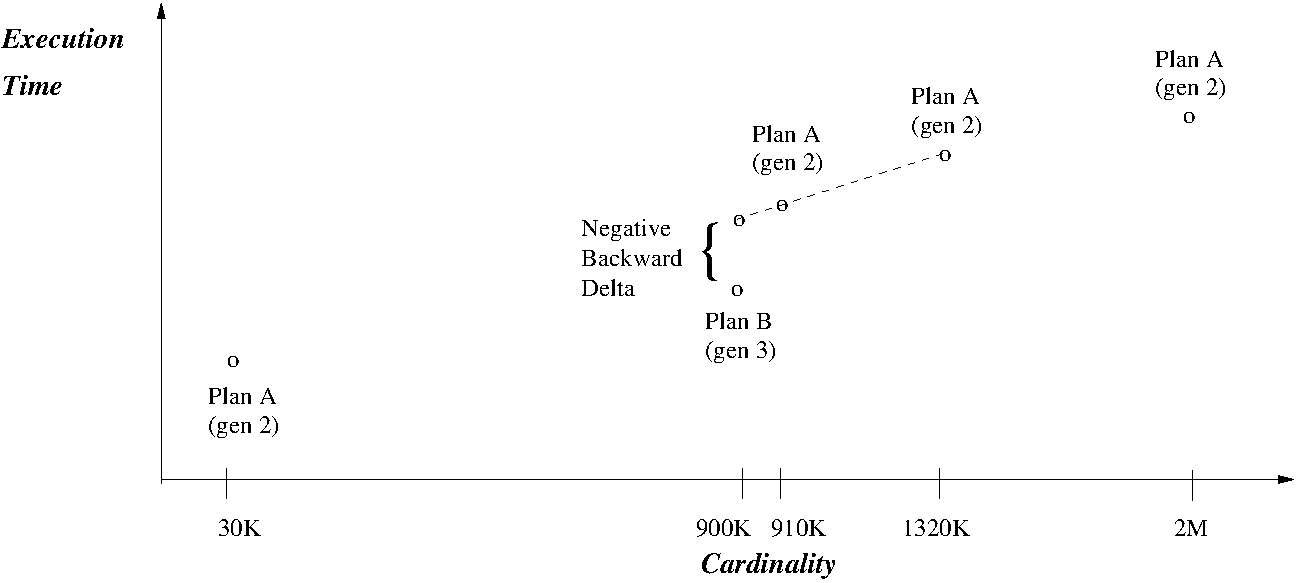
\includegraphics[width=30pc]{figures/negback.pdf}
\caption{An Example of a Negative Backward Delta\label{fig:negback}}
\end{figure*}

In this case, the thinking goes that, had we been
in the \hbox{DBMS} generation 2, the optimizer would have selected Plan A
throughout, because Plan B simply wasn't possible (as it involves an
operator not present in generation 2). Then when generation 3 was created by
adding an operator, the optimizer chose Plan B for 900K. The reason Plan B
was chosen is that it was faster than Plan A at that cardinality, shown in
the figure by extrapolating the run time down from 910K to 900K (we will
revisit this extrapolation shortly).

In this particular case, as just mentioned, Plan B is more appropriate (faster) than Plan A,
but that is not the only possibility. Sometimes the later generation with
more operators available chooses a plan that is slower
than the plan chosen by the earlier generation, due to the suboptimality
we've observed. (We'll examine an example shortly.)

The question then becomes, does a plan change by a subsequent generation
(\hbox{enabled} by the additional operator in that generation) represent a win (runs faster)
or a loss (runs slower)? More broadly, do the Q@Cs
in the aggregate enabled by each successive generation continue to overcome
the increasing burden of suboptimality?

\subsection{Characterizing \hbox{DBMS} Generations}
To which generation do we assign each \hbox{DBMS} operator?

Note that we don't actually know the specific order in which the operators
were added to each \hbox{DBMS}. But even if we did, that order was somewhat
arbitrary, with a host of considerations going into those decisions over the
years. Given that we are using the same optimizer for each such defined
generation, we'll adopt a more systematic ordering of the operators. We
start by gathering all single-operator plans, all two-operator plans,
and so forth, and order the generation by the prevalence of their
\hbox{appearance} in these query plans.

Specifically, for each \hbox{DBMS} we designate the first
generation to contain the single operator that maximizes the number of plans
at change pairs, that is, maximizing the number of Q@Cs, containing just that
operator. So for example, all the plans generated by one DBMS that have exactly
one operator involve just the Full Table Scan operator.  So no choice was
needed: we designate the
first generation as just having that one operator. Any plan with just that
operator can be constructed by generation 1, as well as by any
subsequent generation (as each generation includes that initial operator).

We then examine the plans containing exactly two operators.
Using DBMS A again, there are two such: one with the Full Table Scan and
Full Table Scan with Join operators (888 Q@Cs) and
one with the Full Table Scan and Ref operators (112 Q@Cs). Full
Table Scan with Join is thus the operator added by Generation 2, given its
prevalence of Q@Cs. Each
subsequent generation adds that operator that maximizes the number of plans
that operator will eventual enable. So Generation 3 adds the Eq\_Ref operator,
as that operator enables 633 plans eventually. Generation 4 adds the Ref
operator and Generation 5 adds the Index operator. 

The generations thus can be characterized from the Q@Cs we encountered: five distinct combinations of two
operators, covering 1086 Q@Cs, six combinations of three operators (1126 Q@Cs),
two combinations of four operators (104 Q@Cs), and exactly one
combination of all five operators (6 Q@Cs).\shorten{ Thus for MySQL our data implies
a simulation of five distinct generations, each adding an operator.

\begin{align*}
g_1 &= \{ \hbox{\em full table scan} \}\\
g_2 &= \{ \hbox{\em full table scan}, \hbox{\em scan with join} \}\\
g_3 &= \{ \hbox{\em full table scan}, \hbox{\em scan with join}, \hbox{\em eq\_ref} \}\\
g_4 &= \{ \hbox{\em full table scan}, \hbox{\em scan with join}, \hbox{\em
  eq\_ref}, \hbox{\em ref} \}\\
g_5 &= \{ \hbox{\em full table scan}, \hbox{\em scan with join}, \hbox{\em
  eq\_ref}, \hbox{\em ref}, \hbox{\em index} \}
\end{align*}}
For the four \hbox{DBMSes} in our study, the number of generations ranged from five
to thirteen. 

\subsection{Number of Change Pairs Per Generation}\label{sec:CPQ}
As an illustrative example of how we can look at DBMS query optimizer
performance through the lens of change pairs, let's consider  the {\em
  maximum number of change pairs per query}, or {\em maximum CPQ}, from the
perspective of
\hbox{DBMS} generations.

For each query, we count the number of Q@Cs at each
generation, so for instance a query might have five Q@Cs at generation 1, seven Q@Cs at
generation 2, and 17 Q@Cs at generation 5. We then then take the maximum CPQ
over the queries (so perhaps 17 is the maximum for generation 5 over all
queries). Our hypothesis is that as the generation increases, the maximum
query flutter will increase, which then influences the maximum CPQ. The results are shown in Table~\ref{tab:maxcpq}.

\begin{table}[h]
\tbl{Max Change Pairs Per Query, Per Generation\label{tab:maxcpq}}{%
%\begin{center}
\begin{tabular}{c|cr}
{\em Generation}&{\em Maximum Change Pairs}\\
& {\em Per Query}\\
\hline
1 & 1\\
2 & 66\\
3 & 115\\
4 & 136\\
5 & 132\\
6 & 141\\
7 & 42\\
8 & 172\\
9 & 2\\
10 & 12\\
11 & 55\\
12 & 29\\
13 & 1\\
{\em Cumulative} & 172\\
\end{tabular}
%\end{center}
}
\end{table}

What we notice is that the maximum CPQ does increase with generation,
up through generation 8, after which it falls off dramatically. In
retrospect, this fall-off makes sense. There can be only 200 Q@Cs for a
query, because we look for query plan changes only every 10,000 (300 in one
DBMS) tuples down from
a maximum of 2M (60,000) tuples. As the generation increases, there is less ``room''
for more plans (as some fraction of the previously generated plans will
still be quite good or even optimal), and so less opportunity for flutter
which will show up as a large maximum CPQ. And indeed, at generation 8,
there is a query that has an astonishingly high number of change pairs,
172, all waffling between plans within that generation.
This analysis indicates that there is something concerning change pairs that seems to get
critical around generation 8. We'll return to this in Section~\ref{sec:hitthewall}.

\subsection{Using Change Pairs}\label{sec:usingCP}
We now consider how change pairs can be used to evaluate the
effectiveness of different generations of a \hbox{DBMS}.

Define $\hbox{\em ops}(p)$ for a given plan $p$ to be the set of operators
present in that plan, with some operators perhaps repeated in that plan. 
A plan $p$ is {\em applicable} to a DBMS generation $g$ (denoted by a set of
operators) if $\hbox{\em ops}(p) \subseteq g$. By
definition, if a generation is applicable to a given plan, it is
applicable to all subsequent generations, with one being the 
{\em earliest applicable generation}, or {\em mingen}.
\shorten{
\shorten{We couldn't make this one work...
\todo{Young:replace in the above para with an actual SQL example query that was associated
  with two MySQL generations in a Q@C pair. use the generation numbers from
  the next para} 

\todo{Rick: I found one example but the cardinality information 
was different than what's stated in the current prose...}

%%runid = 1097, querynum = 46, max_card = 60000, upper_card = 29100, lower_ard = 28800, upper_gen = 4, lower_gen = 5
%%max_cqt: 230, upper_cqt: 110, lower_cqt: 120, lower_extrapolated_cqt: 110
%% experimentname: op-pk-30K-100q-idx, pk: true, sec_idx: true
%% plan 0: ALL:Full Table Scan,ref
%% plan 1: eq_ref,index,ref
%% plan 0 at upper_card, plan 1 at lower_card
\noindent
\hspace{3ex}{\small\begin{verbatim}
        SELECT t3.id2, t3.id4, t0.id3, t2.id1 
        FROM ft_HT3 t2, ft_HT1 t1, ft_HT2 t3, ft_HT1 t0  
        WHERE  (t2.id2=t1.id2 AND t1.id2=t3.id1 AND t3.id1=t0.id4)
\end{verbatim}}
}
}
For each change pair, containing adjacent Q@Cs, we have either one or two
generations to consider. We focus on change pairs with two generations, and start with
those for which $\hbox{\em 
mingen}(\hbox{\em lower}) > \hbox{\em mingen}(\hbox{\em
  upper})$. An example is shown in Figure~\ref{fig:posback}. In this case,
the set of operators in Plan A for the Q@C at cardinality 900K requires at
least generation 3, whereas the set of operators for Plan B for the Q@C at
cardinality 910K requires generation 2. (Note that the generations in
this example
are consecutive, but that is not required. Sometimes the generations within a
change pair are quite different, such as generation 2 at the lower plan of a
pair but generation 5 at the upper plan.)

\begin{figure*}[t]
%\centering
%originally 30pc
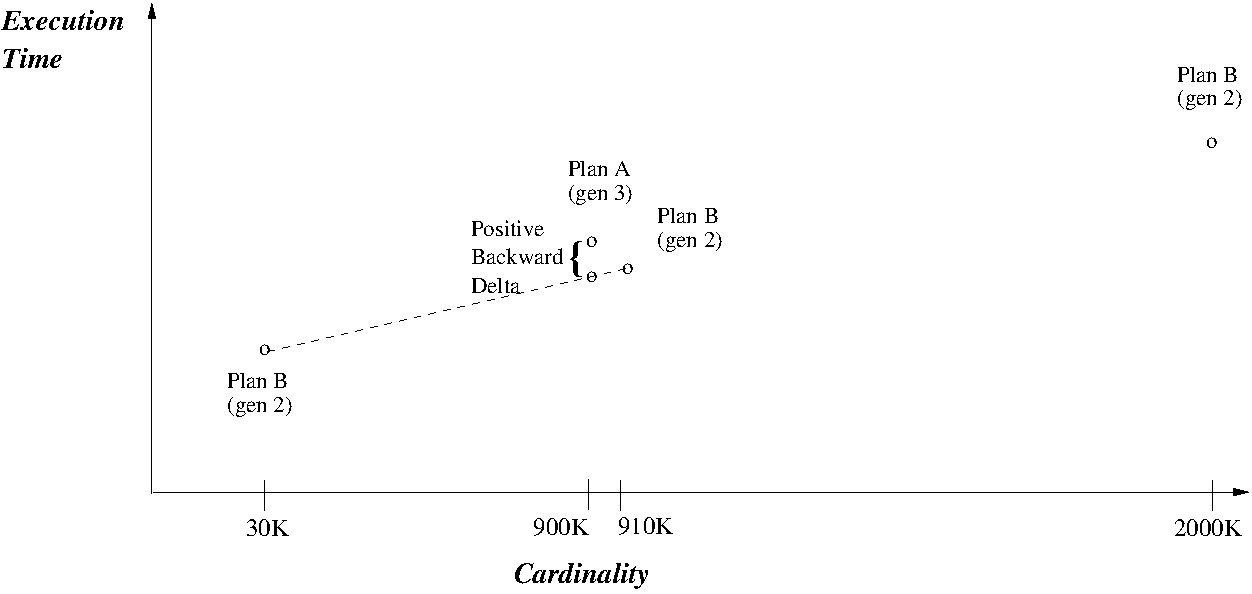
\includegraphics[width=30pc]{figures/posback.pdf}
\caption{An Example of a Positive Backward Delta\label{fig:posback}}
\end{figure*}

To examine the wisdom of picking Plan A for 900K (whose run time was measured as
the higher point pair shown, the one above the dashed line), we find the closest Q@C
also having Plan A. There are two illustrated here, at cardinalities 30K and
2000K, respectively, with the closer one at 30K. (If there is no such Q@C,
we can't do the extrapolation, and simply remove that change pair from
further consideration.)

We then extrapolate the measured time for the closest plan of the lower
generation to the cardinality of the adjacent higher generation. In this
particular case, we use the measured query time of Plan
B at cardinalities 30K and 910K to extrapolate an estimated query time at 900K.
This realizes an estimate of how fast the query using Plan B would have run
on the database having the variable table with a cardinality of 900K. In
this particular case, Plan B looks like it would have run {\em faster} (in
fact, was faster even at 910K in this particular example).

\discont{As illustrated in Figure~\ref{fig:discontinuity}, plans can be
discontinuous, an example being external merge sort. For that operator}{Note
  that for some operators, such as external merge sort}, as
the cardinality increases, an additonal pass may at some point be needed,
but the query time will be roughly linear for a set number of passes.
Returning to the situation in Figure~\ref{fig:posback}, the presence of a change in the number of passes, say between 30K and 910K,
will have the effect of flattening the slope slightly for Plan B, such that
this extrapolation will slightly underestimate the run time of
that plan at 900K, and thus overestimate the penalty of going with
Plan A rather than Plan B. That said,
given that we are extrapolating from the actual run time at a very
close cardinality, our extrapolated estimate should be similarly close.

We term this situation a {\em backward extrapolation}, because we are extrapolating
backward from a cardinality of 910K to one of 900K, within the change pair.

With this extrapolation, we can compute, for each change pair, the {\em relative delta}, defined as the
measured time of Plan A (the chosen one) at the lower cardinality (here, 900K) minus the
extrapolated time of Plan B at that same cardinality, divided by the
larger of the measured and extrapolated time of the plan at the higher
generation (here, Plan A). The relative delta is thus scaled by original
measured time at that granularity, and thus has a maximum possible value of 1.

In this case, the relative delta is positive (the measured time for the plan
associated with the higher generation is greater than the extrapolated
time), which indicates that the optimizer chose a slower plan: here,
Plan B should have been chosen.  

On the other hand, a {\em negative} relative delta (where the measured
time for the plan associated with the higher generation is lower than the
extrapolated time, such as that illustrated in Figure~\ref{fig:negback})
implies that the additional operator(s) available to the minimally
applicable generation of the upper plan were indeed beneficial, in that that
plan was faster. (In such cases, we again divide by the larger
value, so the minimum possible value is~-1.)

Summarizing, this analysis computes, for a {\em change pair} (a pair of
adjacent Q@Cs for a specific query running on a specific DBMS), a {\em
  relative delta} for the earliest applicable generation. A
positive relative delta (extrapolated in either the forward or backward
direction) reflects that a slower
plan was chosen by the \hbox{DBMS} generation, perhaps due to the greater number of
operators available. A negative relative delta (forward or backward) reflects
that the chosen plan was faster at that cardinality than the one
chosen at the adjacent cardinality.

There are ten orthogonal possibilities for each change pair (that
is, a pair of adjacent Q@Cs), a total of 66,792 change
pairs from the Exploratory and Confirmatory Experiments. (There is also the
case of a query instance containing a lone Q@C, meaning that only one plan was
chosen across all 200 Q@Cs. This occurred for 2126 out of the 8840
query instances, which we don't consider further.)

\begin{enumerate}
\item The pair of Q@Cs share the same generation: $\hbox{\em mingen}(\hbox{\em lower}) =
\hbox{\em mingen}(\hbox{\em upper})$  (62,903 change pairs, or 94.2\% of the
total), which we don't consider further.

\item The extrapolation yielded a computed query
time that was negative, which we also drop (10 change pairs, 0.01\%).

\item The extrapolation was from above and indicated
no suboptimality, termed a {\em negative backward relative
  delta}, as
  exemplified in Figure~\ref{fig:negback}, examined earlier (583 change pairs,
  0.9\%).

\item The extrapolation, termed a {\em positive backward
    relative delta} and exemplified in Figure~\ref{fig:posback}, indicated
  a suboptimal plan (492 change pairs, 0.7\%).

\item The extrapolation was a {\em negative forward relative delta},
  indicating no suboptimality (795 change pairs, 1.2\%).

\item A extrapolation was from below (consider Figure~\ref{fig:negback} but with
  Plan A from generation 5; we would then need to extrapolate from the
  closest Plan B, which is {\em at a smaller cardinality}), in a {\em forward
    direction}, to compute a {\em positive forward relative delta},
  indicating a suboptimal plan (1218 change pairs, 1.8\%).

\item The pair had an upper plan that was newer but no forward extrapolation
  was possible (554 change pairs, 0.8\%).

\item The pair had a lower plan that was newer but no backward extrapolation
  was possible (224 change pairs, 0.3\%).

\item The pair had a relative delta of -1 (2 change pairs, 0.002\%).

\item The pair had a relative delta of 1 (11 change pairs, 0.01\%).

\end{enumerate}
%1 of rel del: 2, -1 of rel del: 21 (neg backward:3, pos backward:18)
From these ten possibilities, we thus retain (3) and (5), which indicate a
faster plan at the later generation (1378 pairs: not suboptimal), and (4) and (6), which indicate a
slower plan at the later generation (1710 pairs: suboptimal).

\subsection{Realizing the Gedanken Experiment}\label{sec:realizing}
We now have the components in place for performing an experiment that
parallels the Gedanken experiment described in Section~\ref{sec:gedanken}.

The analysis in the previous section is for {\em a single pair of adjacent Q@Cs for a single query
running on a specific \hbox{DBMS}},
providing a {\em relative delta} for the minimally \hbox{applicable} generation. A
positive relative delta indicates that the later generation chose a
suboptimal plan; a negative relative delta indicates the later generation
did not. The relative delta is a percentage difference, and so is not \hbox{affected}
by the absolute magnitude of the run time nor by the cardinality in
question. Indeed, because it is a percentage difference, the relative delta
is not affected by the query nor even which \hbox{DBMS} is involved. (DBMSes
vary greatly in the estimated time of individual queries; using the actual
query time would artificially give more weight to change pairs from the
slowest DBMS.) We associate
this relative delta with the later generation, for it is that generation
which had the choice between the two plans for that query.

Consider how the {\em average} relative delta, computed across queries and
DBMSes, of query plans associated with that individual generation, might
behave across successive generations.
The average relative delta for an individual generation is a characterization of the
aggregate impact of the query plans associated with that generation, providing a quantitative estimate of the benefit
of adding that operator. (We use average so that each point is not impacted
by the number of change pairs over which that point is computed. Note that
this approach weights the queries equally. This makes sense for our queries,
summarized in Section~\ref{sec:experiments}; those queries are quite similar.)

What does our causal model in Figure~\ref{fig:model}, supported by the
correlational and regression analyses of the Confirmatory Experiment in
Sections~\ref{sec:corr} and \ref{sec:regression}, say about this? That
causal model asserts that as the number of operators increases in
subsequent generations, the intervening measures in plan space complexity increase, which
therefore impacts suboptimality, also in a positive direction.

Our Gedanken experiment in
Section~\ref{sec:gedanken} takes this behavior and predicts that
as the generations contain successively greater numbers of
operators, optimizer missteps will increase and possibly dominate. What is
the correspondence with the realizable experiment we are now considering?

If we plot the performance of the DBMS on the {\em y}-axis for a
workload consisting of a set of queries over a 
prescribed data set, for a sequence of DBMS generations arranged on the
{\em x}-axis, the average relative delta is in some way a characterization
of the {\em slope} of this relationship. A negative average relative delta
implies that the indicated generation is doing a good job, with less
suboptimality, and so the total workload execution time will go down and
performance will go up; a
positive average relative delta implies that the suboptimal decisions are
dominating, indicated by the total workload execution time going up for that
generation, and thus performance going down.

We expect that the average relative delta for the first few
generations will reflect new operators that improve some
plans, a natural result of the \hbox{efforts} of \hbox{DBMS} developers to
increase performance over successive generations of their \hbox{DBMS}.

That said, all is not rosy in this picture. Each new operator is applicable
to a successively smaller portion of the queries, and perhaps over a
successively smaller portion of the cardinality space.  As already noted,
our causal model predicts that the prevalence of suboptimality will
increase as operators are added.  It seems that even
with DBMS implementers doing smart things, these two considerations predict
that the average relative delta 
will  increase, as suboptimality (a positive relative delta) becomes
more prevalent. This analysis suggests then that the performance curve will
level off and then start dropping off.

So the question comes down to this:  {\em Is there an empirically-determined
point where the decrease due to suboptimality obviates the increase enabled
by the new operator: a DBMS generation where the performance actually drops,
as predicted? How close might modern \hbox{DBMSes} be to that limit?}

\subsection{Trends Across DBMS Generations}\label{sec:trends}
We partition the relevant four sets of change pairs discussed in the
Section~\ref{sec:usingCP} into two groups. The first group consists of those
change pairs with a {\em positive}
relative delta (either forward or backward), indicating that the query
optimizer selected a slower plan at the later generation (corresponding to a
higher generation number), thereby denoting an (empirically) {\em suboptimal
  decision} by the query optimizer at that later generation. The second
group consists of those change pairs 
with a {\em negative} relative delta (either forward or backward) relative
delta, indicating that the query optimizer selected a faster plan at the
later generation, which was thus an (empirically) {\em non-suboptimal
  decision} at that later generation. Note that we can't state
unequivocally that the plan will a negative relative delta is optimal (in the
original, absolute, sense of that term) because there may be a yet another
plan involving the operators 
within that generation that is even faster. That said, in the other case, a positive relative
delta reliably asserts that the plan at this Q@C is \hbox{demonstrably}
{\em empirically suboptimal}, and thus also is suboptimal in the absolute case.

\begin{table}[t]
\tbl{Beneficial Change Pairs\label{tab:non-subopt}}{%
%\begin{center}
\begin{tabular}{c|c|c|c}
{\em Generation}&{\em Number of} &{\em Average}&{\em Cumulative}\\
& {\em Change Pairs} & {\em Relative Delta} & {\em Relative Delta}\\
\hline
1 & --- & --- & 0.00\\
2 & --- & --- & 0.00\\
3 & --- & --- & 0.00\\
4 & 24 & -0.28 & -0.28\\
5 & 282 &-0.118 & -0.130\\
6 & 309 &-0.274 & -0.203\\
7 & 336 & -0.317 & -0.243\\
8 & 43 & -0.20 & -0.241\\
9 & 4 & -0.1 & -0.241\\
10 & 17 &-0.29 & -0.241\\
11 & 357 & -0.178 & -0.225\\
12 & 6 & -0.2 & -0.225\\
13 & 0 & --- & -0.225\\
{\em Cumulative}  &1378 & ---& -0.225\\
\end{tabular}
%\end{center}
}
\end{table}

\begin{table}[t]
\tbl{Deleterious Change Pairs\label{tab:subopt}}{%
%\begin{center}
\begin{tabular}{c|c|c|c}
{\em Generation}&{\em Number of} &{\em Average}&{\em Cumulative}\\
& {\em Change Pairs} & {\em Relative Delta} & {\em Relative Delta}\\
\hline
1 & --- & ---   & ---  \\
2 & --- & ---   & ---  \\
3 & --- & ---   & ---  \\
4 & 2   & 0.2   & 0.2  \\
5 & 211 & 0.076 & 0.077\\
6 & 86  & 0.16  & 0.102\\
7 & 263 & 0.303 & 0.196\\
8 & 273 & 0.303 & 0.231\\
9  & 3  & 0.04  & 0.230\\
10 & 168& 0.319 & 0.245\\
11 & 639& 0.237 & 0.242\\
12 & 53 & 0.35  & 0.245\\
13 & 12 & 0.40  & 0.246\\
{\em Cumulative}&1710&---&0.246\\
\end{tabular}
%\end{center}
}
\end{table}

We first examine those change pairs for which the query optimizer made a
good \hbox{decision}: the non-suboptimal change pairs, summarized in
Table~\ref{tab:non-subopt} and designated as {\em beneficial}.
This data aggregates the results over the
four \hbox{DBMSes}, which had generations ranging from five to thirteen. Overall, only a small number of change pairs, 1378, or about 2\% of the
total, satisfied the requirements listed in Section~\ref{sec:usingCP}, including having a different
generation number for the lower and upper plans. In fact, there were no such
change pairs for the first three generations nor for the last
generation. The second column states the number of change pairs added by
that generation and the third column the average relative delta across just those change
pairs. The last column states the {\em cumulative relative delta} for that
generation, defined as
the sum of the average relative delta for those change pairs associated
with plans having only operators in its generation, divided by the number of such
change pairs. It thus
includes the change pairs associated with all previous generations,
again, as those plans all include operators made available by that generation.

The averages jump around quite a bit, especially for the first few
generations. (One of the reasons is that the number of change pairs
associated with an individual generation varies a
lot.) \hbox{Focusing} on the last column, we see that the cumulative
relative delta starts off at a low of
-0.28 (recall that a negative value is good, as it indicates the
additional operator was effective at lowering the query time) and slowly
increases to -0.225, or more negative numbers trending to less negative
numbers, indicating decreasing benefits of optimization.

This general behavior matches our prediction arising from the structural
causal model: it gets harder for the DBMS query optimizer to squeeze out
performance gains as operators are added to the \hbox{DBMS} over successive
generations.

We now examine those change pairs for which the query optimizer made a poor
decision, in that we can conclude that there was a better plan (the one
right next to it in the change pair), designated as {\em deleterious}. Table~\ref{tab:subopt} provides the
same information across the \hbox{DBMS} generations for the suboptimal
change pairs: those for which the relative deltas are positive, indicating a
decision that increased the query time. While there are still only a small
number of such change pairs, there are more deleterious than beneficial
pairs, with a relatively greater number showing up at more recent
generations. (Half of the beneficial change pairs occurred before generation
8, but half of the deleterious change pairs showed up only in generation 10
or higher.) More strikingly, the cumulative relative delta has the opposite
behavior to the \hbox{non-suboptimal} change pairs (which showed decreasing
benefits): it {\em increases} over the generations (indicating greater
suboptimality), starting at 0.077 and ending at 0.246, a value {\em higher}
than that of the non-suboptimal change pairs. Both trends were as predicted.

\subsection{Have Modern DBMSes Hit The Wall?}\label{sec:hitthewall}
Table~\ref{tab:performance} brings the beneficial and deleterious change
pairs together, stating the total number of change pairs associated with
each generation and the {\em average net relative delta}, again, just for
change pairs associated with that generation. Note that in the third column,
the average net relative delta (per generation), the values transition from
negative (indicating better performance), to quite positive (worse
performance); recall that the relative delta is bounded by -1 and 1.

\begin{table}[t]
\tbl{Assembled Change Pairs and Relative ``Performance''\label{tab:performance}}{%
%\begin{center}
\begin{tabular}{c|c|c|c}
{\em Generation}&{\em Number of} &{\em Average Net}     &{\em Cumulative Net}\\
            & {\em Change Pairs} & {\em Relative Delta} &{\em Relative Delta}\\
\hline
1           & ---                & ---                  & ---\\
2           & ---                & ---                  & ---\\
3           & ---                & ---                  & ---\\
4           & 26                 & -0.24                    & -0.24\\
5           & 493                & -0.035                    & -0.045\\
6           & 395                & -0.179                    & -0.103\\
7           & 599                & -0.045                    & -0.0800\\
8           & 316                & 0.235                    & -0.0256\\
9           & 7                  & -0.04                    & -0.0257\\
10          & 185                & 0.263                    & 0.00750\\
11          & 996                & 0.088                    & 0.0296\\
12          & 59                 & 0.29                    & 0.0346\\
13          & 12                 & 0.40                    & 0.0360\\
{\em Cumulative}& 3088           & ---                  & 0.0360\\
\end{tabular}
%\end{center}
}
%\todo{Young: could you provide the third column? It's the average just for
%  the change pairs for that generation.}
\end{table}

The final column in Table~\ref{tab:performance} provides the
cumulative net relative delta.  This column thus reflects all the change pairs
with plans that would have been generated by that DBMS generation
(hence, including change pairs at that generation along with those
at previous generations). This value provides an indicator of how the four
\hbox{DBMSes} together would have performed (say, in total execution time) on the
workload of the Exploratory and Confirmatory
Experiments, or rather on the 3088 change pairs selected by the criteria in
Section~\ref{sec:usingCP}. (We emphasize that our experiment estimates with
empirical results just
the first derivative of the performance graph, the cumulative net 
relative delta, and then only for a small
number of Q@Cs, and then only as a relative measure, between -1 and 1. It is
thus only very roughly indicative of the {\em shape} of the performance
graph.)

We see that the cumulative net relative delta starts out \hbox{at -0.24}, indicating
that the new operators are {\em increasing} the performance (by
{\em decreasing} the query time) for the workload. This happy situation
unfortunately starts to deteriorate: after generation 6, with each
successive generation, the performance deteriorates. This is as predicted:
the optimizer is struggling with both more options (plans over the available
operators) to select from and a diminished opportunity to make a significant
improvement.

\shorten{OLD: The final column of Table~\ref{tab:subopt} integrates the
  average relative delta to produce a unit-less
{\em relative performance}, an indicator of how the four DBMSes together
would have performed (say, in total execution time) on the workload of the
Exploratory and Confirmatory
Experiments, or rather on the 1378 change pairs selected by the criteria in
Section~\ref{sec:usingCP}. (We emphasize that our experiment estimates just
the first derivative of the performance graph, the average relative delta, and then only for a small
number of Q@Cs, and then only as a relative measure, between -1 and 1. It is
thus only very roughly indicative of the {\em shape} of the performance graph.)
The relative performance gets better (faster, indicated by a falling
value), but that trend again stops at generation 10, after which the
relative performance actually gets worse (slower, indicated by a rising value).}

\begin{figure}
    \subfigure[Cumulative Relative Deltas]{
        %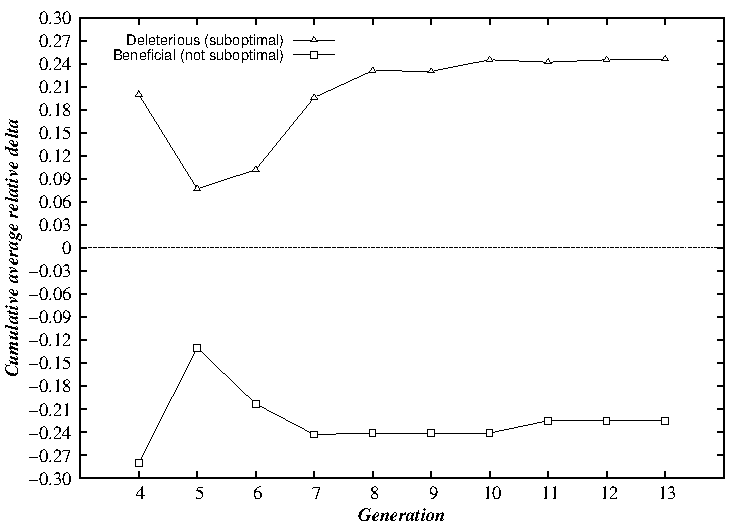
\includegraphics[width=20pc]{figures/gen_benefit.pdf}
        %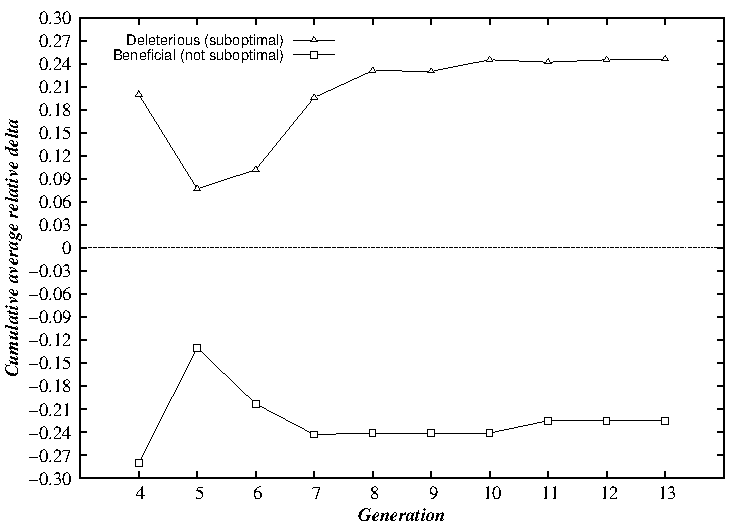
\includegraphics[scale=0.56]{figures/gen_benefit.pdf}
        %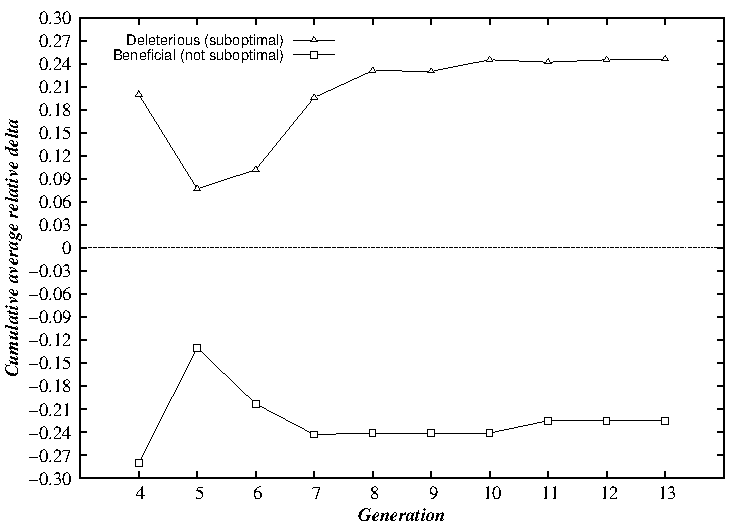
\includegraphics[width=19pc, height=5.5cm]{figures/gen_benefit.pdf}
        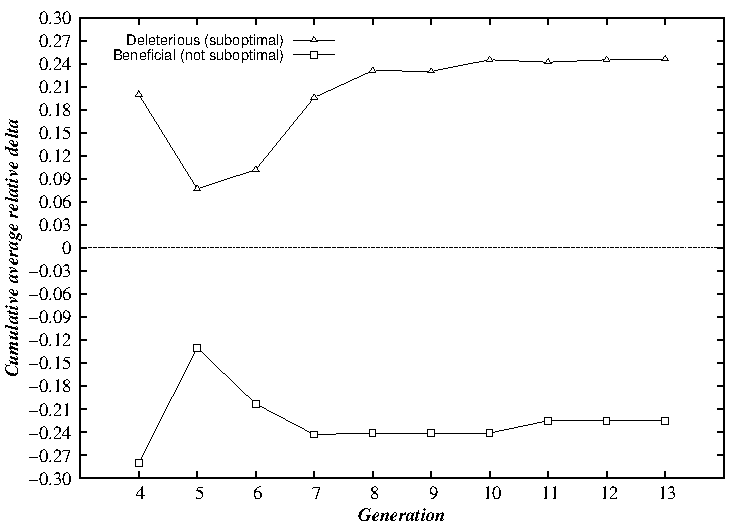
\includegraphics[scale=0.735]{figures/gen_benefit.pdf}
        \label{fig:benefit}
    }
    \hspace{-0.17in}
    \subfigure[Performance over Generations]{
        %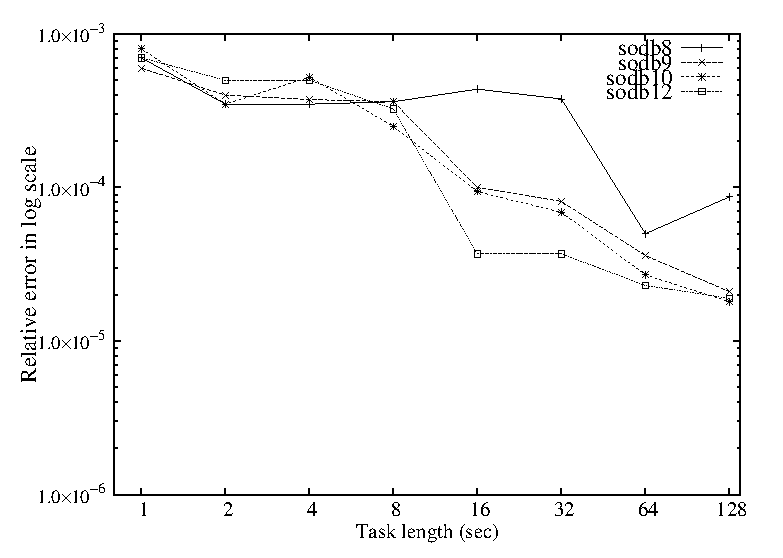
\includegraphics[scale=0.6]{overall/machine_pt_re.eps}
        %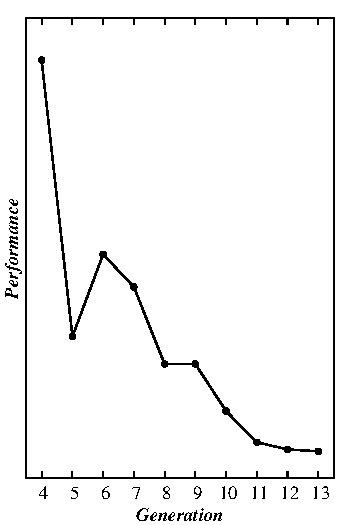
\includegraphics[width=12pc]{figures/perf_gen.pdf}
        %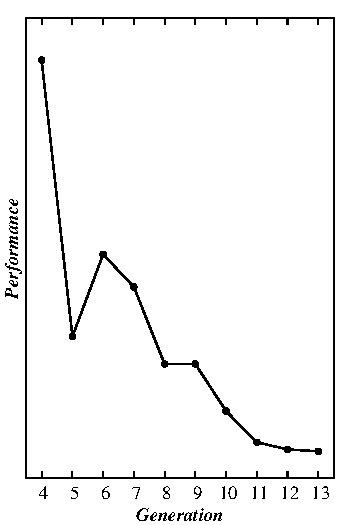
\includegraphics[scale=0.56]{figures/perf_gen.pdf}
        %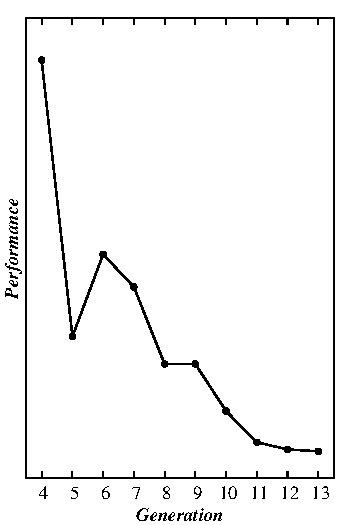
\includegraphics[width=14.5pc, height=5.5cm]{figures/perf_gen.pdf}
        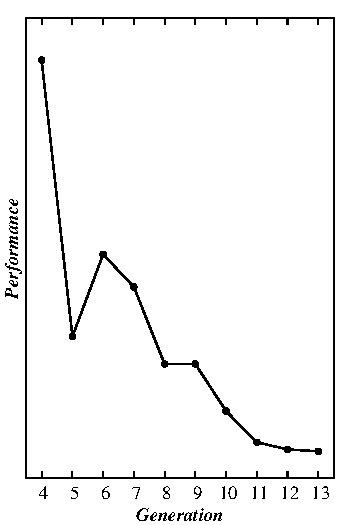
\includegraphics[scale=0.735]{figures/perf_gen.pdf}
        \label{fig:performance}
    }
%\todo{Young: Please remove the ``Net Cumulative Relative Delta'' curve in
%  the middle and instead put it as 10(b).}
%\todo{Young: also replace ``Suboptimal'' with
%  ``Deleterious (suboptimal)'' and ``Not suboptimal'' with ``Beneficial (not suboptimal)''}
    \caption{Trend of Relative Performance over Generations}
    \label{fig:machine_comp}
\end{figure}

Figure~\ref{fig:machine_comp} tells the story
graphically. Figure~\ref{fig:benefit} plots the last column of
Table~\ref{tab:non-subopt} as the bottom line (beneficial: non-suboptimal cumulative
relative delta) and the last column of Table~\ref{tab:subopt} as the top
line (deleterious: suboptimal cumulative relative delta).
Figure~\ref{fig:performance} plots the ``Relative Performance'', that is,
the negation of the cumulative net relative delta (as a positive relative
delta denotes a slower query, reflecting decreased performance) appearing as the
last column of Table~\ref{tab:subopt}, as this characterizes the relative
performance across generations. This line has a least squares slope of
-0.024.

\subsection{Summary}
The engineering perspective in Section~\ref{sec:gedanken}
predicts that the overall per-generation run time would ``monotonically decrease
as the generations add query evaluation operators.'' The scientific
perspective, applying our validated causal model, reaches the opposite
conclusion: there will be a point where ``the
\hbox{increase} in execution time due to suboptimality obviates the decrease
enabled by the new operator.'' The results of this study clearly support
the latter (cf.~Figure~\ref{fig:performance}).

This highly aggregated result, extracting 3000-odd change pairs having
the specified properties of interest stated in Section~\ref{sec:usingCP} and
drawn from over \hbox{100,000} Q@Cs implies that these four
particular \hbox{DBMSes}, taken together, might be close to or have already
hit the wall, where adding an operator actually slows down the average
query. And recall the analysis in Section~\ref{sec:CPQ} in which a
related problem cropped up around generation 8.  This is the
first study we are aware of that compares the generational trends of
\hbox{DBMSes} over quite disparate code bases, thus getting at fundamental
trends. 

It is important to emphasize that we can't say from this one study
whether any of these DBMSes have actually
transitioned to where, for this class of queries, the cost of the
suboptimal change pairs overwhelm the benefits of the non-suboptimal change
pairs. Presumably, the DBMS vendors have done extensive tests to ensure
that the operator added to each generation did in fact effect a speedup on
the representative workloads that they use in evaluating their optimizer
enhancements. However, we {\em can} say that (a)~the trends observed
strongly point to a decreasing benefit and an increasing cost, as predicted
by the simple arguments made above, and (b)~if current DBMSes haven't yet
reached the point of diminishing returns, that possibility looms in the future.

We reiterate the provisos mentioned earlier. In all of these
experiments, we are looking at quite simple queries, over a quite limited
range of data, with only a small percentage (3\%) of change pairs
identified in our experiments. On the other hand, simpler queries
are thought to be easier to generate good plans than more complex queries
(as Hypothesis 2 in Section~\ref{sec:hypotheses} states). Also, relational
data is generally much less uniform in its (i)~data types (we used only
integer data), (ii)~values (the values in our tables are quite evenly
distributed), (ii)~schemas (the schemas of our tables are identical and
quite simple), and (iii)~range of table cardinalities (our smallest
table is $1/{200}^{th}$ of the largest table). The simplicity of queries, schemas,
and tables in this study should independently, and certainly in concert,
minimize the suboptimality observed. Thus, more complex workloads may
present an even higher degree of empirical suboptimality.

\section{Engineering Implications}\label{sec:engineering}
We studied a particular
phenomenon, suboptimality, when the \hbox{optimizer} selecting a slower
plan. This phenomenon is indicated by the existence of a query plan that performs more efficiently
than the DBMS's chosen plan, for the same query. From the engineering
\hbox{perspective}, it is of critical importance to understand the prevalence
of Suboptimality and its causal factors. The genesis of our predictive model
was a sense that Suboptimality is caused in part by the inherent complexity
of these systems and the concomitant interactions between various rules in the
optimizer.

Through a series of experiments managed by our laboratory instrument
management system, \azdb, carried out across several years, we uncovered
several surprising results that provide systematic clues as to where current optimizers come up
short and how they can be further improved.

\begin{itemize}
\item For many queries, a majority of the ones we
considered, the optimizer picked a slower plan for at least one
cardinality, even when the cardinality estimates were completely accurate
and even for our quite simple queries.

\item A quarter of the queries exhibited significant suboptimality ($\geq 20\%$ of
        the run time) at some cardinality.
\end{itemize}
\noindent
These two results indicate that there is still research needed on
this topic. Fortunately, the causal model can suggest
specifically where that research should be focused.

\begin{itemize}

\item Many queries exhibited {\em query fluttering}, in which the query
  optimizer returned to a previous plan at a higher cardinality.
\item Some queries exhibited significant {\em query thrashing}, with a plan change at
         almost every cardinality. While this phenomenon was first visualized
         by Haritsa et al.~\cite{harish07,Haritsa10} on some complex
         queries, we have shown that it is present even in a surprising
         percentage of simple queries.

\item Furthermore, some queries exhibited many changes
{\em to a suboptimal plan} as the \hbox{cardinality} was varied.
\end{itemize}
\noindent
These particular queries, as well as those of the right-hand side of
Figure~\ref{fig:suboptcumulative} exhibiting a large degree of suboptimality, can be a starting point for identifying the root
cause(s) of query thrashing. The phenomenon can be investigated initially on a
per-DBMS basis. Our methodology could then be
used to test proposed causal mechanisms of query thrashing across \hbox{DBMSes}, to
ascertain the generality of any proposed solutions.

\begin{itemize}
\discont{\item The causal model and our experimental results suggest that more
research is needed to improve the cost model of {\em discontinuous
operators}.}{}

\item \discont{We also show that it}{It} may well be useful to explicitly take {\em \hbox{cardinality} estimate
  uncertainty} into account. (Leis et al.~\doubleblind{independently }{}came
  to the same conclusion: ``The results ... demonstrate that the
  state-of-the-art in cardinality estimation is far from
  perfect.''~\cite{Leis15}).

\item This research indicates that aggregates are less of a problem, so
  that aspect of query optimization is in reasonable shape.

\shorten{REVISE to characterize
  more precisely the relative
advantage or disadvantage of heuristic search\shorten{, and \hbox{(c)~research} is needed to
identify the inflection point where adding an operator decreases overall
\hbox{DBMS} performance}raise several unsettling concerns. These particularly simple
queries used only a few plans within any \hbox{DBMS}. Other more complex queries
will certainly use more plans. These results imply that as a \hbox{DBMS} becomes
more sophisticated, by adding operators, it also become more unstable, as
the prevalence of suboptimality grows. Perhaps there is a fixed level of
complexity beyond which a cost-based optimizer will be inexorably unstable.}
\end{itemize}

\discont{We see that costing of \hbox{discontinuous} operators is a
root cause of query suboptimality, and is thus particularly challenging to a
query optimizer. If the cost model is even a little bit off, the optimizer
might be on the wrong side of the ``jump'', thereby selecting a slower
plan.  That the Presence of discontinuous operators has such a high
regression coefficient provides a quite specific guideline: more research is
needed to improve the accuracy of the cost model for such operators, such as
careful calibration that tunes the cost model with more accurate resource
knowledge, including the global memory capacity available, as well as to
improve the algorithms that allocate those buffer pages to specific
operators.}{}

Concerning the plan search
process, which was another identified root cause of suboptimality,\shorten{one preliminary finding was that a heuristic
search process was implicated in 10--20\% of optimizer variance.} in cases
where the \hbox{DBMS} is not as sure about the cardinalities of the underlying
relations or the speed of the disk (e.g.,~if such relations migrated
frequently to a different disk drive~\cite{reiss03}), 
perhaps the optimizer should\shorten{not try as hard to produce out the ``perfect'' plan. 
It might help if optimizers instead}
explicitly take uncertainty into account. Indeed, others have started to
\hbox{argue} that uncertainties in the query planning process should be
acknowledged and exploited~\cite{Babcock05}.

We mentioned dynamic query optimization in Section~\ref{sec:related}
earlier.  Dynamic query-reoptimization normally requires a significant
amount of information to be recorded during query execution, which can incur
non-negligible overhead on the overall query
performance~\cite{Avnur,kabra98}.  We envision that by utilizing the
proposed predictive model for suboptimality, it may be possible to enhance
reoptimization techniques such that given a particular query, a particular
data distribution, and a specific plan operator, just the important
statistics that affect the operator's performance can be identified and
should be recorded, thereby reducing the overhead of bookkeeping irrelevant
\hbox{information}.

Hence, the methodology introduced in this paper suggests fairly specifically where additional
engineering is needed (\discont{the cost model of discontinuous
operators and }{}accommodating cardinality estimate uncertainty) and is not
needed (costing of aggregation).

The generational study in Section~\ref{sec:diminishing} though implies that
the challenge in daunting. That study validates the implications of the
causal model in Figure~\ref{fig:model}, which correctly predicts the almost
inexorable rise in per-generation assembled relative delta, which implies that the
optimizer will eventually hit the wall where it is no longer improving.

We emphasize that this section of this paper, considering engineering
implications of the underlying causal model, contrasts with the rest of the
paper, whose focus is on the science and on understanding these complex
systems at a fundamental level.  Good engineering should be built on solid
scientific results. This paper focuses on the latter.

\section{Summary}\label{sec:summary}

This paper studies an important
component of a \hbox{DBMS}, the query optimizer. This component is an amazingly
sophisticated piece of code, but is still not well understood after decades
of research and development.

While there has been a wealth of research over the last forty years on
engineering approaches and refinements to improve the performance of query
optimization, this is the first paper to the authors' knowledge to take a
scientific approach (in the sense of {\em empirical generalization}),
towards the important phenomenon of {\em suboptimality}.

This paper makes the following contributions in
an \hbox{attempt} to gain new understanding of this
component.
\begin{itemize}
\item Shows that even for simple queries, over a simple schema and
  relatively small range of table sizes, the prevalence of {\em query
  suboptimality}, {\em query flutter}, and {\em query thrashing}, three
  problems that have not been systematically investigated across multiple \hbox{DBMSes}, is
  high, and thus there is still research needed on this mature topic of
  query optimization.

\item Introduces a new {\em methodological
perspective} that treats \hbox{DBMSes} as experimental subjects within empirical generalization.

\item Proposes {\em operationalizations} of several relevant measures that apply
  even to proprietary \hbox{DBMSes}, as well as an overarching {\em predictive
    model} that attempts a causal explanation of suboptimality, encoding
   some of what is known about query optimization.

\doubleblind{\item Utilizes a novel {\em research infrastructure}, \azdb, to express, run, and
  analyze experiments.}{}

\item Tests {\em six hypotheses} deductively derived from the predictive causal model. A
correlational analysis and a regression analysis
provided {\em strong support} for our model, across \hbox{DBMSes}, thus
confirming what was informally articulated but never
coherently tested.

\item Uncovers compelling {\em evidence}
(i)~that (empirical) suboptimality correlates with four operationalizations of query complexity,
(ii)~that suboptimality correlates with \discont{three}{two} operationalizations of plan space
complexity,
(iii)~that the Presence of secondary indexes is a contributor to plan space
\hbox{complexity,}
(iv)~that schema complexity, as operationalized by the
Presence of secondary indexes, moderates these \discont{three}{two}
interactions (though weakly and in the opposite direction), and
(v)~that the Presence of skewed data may diminish
Suboptimality slightly.

\shorten{\item A separate analysis suggested that heuristic plan selection
  appears to also be a source of suboptimality.}

\item Explains a {\em significant portion} (\discont{53.6\%}{52.2\%}) {\em of the variance of empirical suboptimality} for the kinds of queries we looked at, based on the interactions as well as the factors that we identified in the model: optimizer complexity, query complexity, and plan space complexity.  No other factor, as yet unknown, nor combination of factors,
will themselves predict as much variance as the factors we studied in this
paper. And somewhat extraordinarily, it is these common aspects that predict
suboptimality, not the particulars embedded in the inordinate complexity of
each of these DBMSes.
That said, it is certain that there remain several unknown causal factors;
identifying those factors may also have important engineering
implications.

\item Articulates for the first time a {\em limit} on the
  number of operators a \hbox{DBMS} may be able to support, given that the
  empirical evidence suggests that additional operators speed up a smaller
  and smaller portion of the query/cardinality space while incurring an
  increasing chance of suboptimality over the remaining space, which is
  growing.

\item Applies a novel experiment over pairs of adjacent Q@Cs, providing
  empirical evidence that {\em this limit exists} and may have already been
  reached by one or more our subject DBMSes.

\item Identifies {\em specific directions for engineering interventions}.

\item Provides a {\em path toward scientific progress} in the understanding
  of a key enabling technology.  It is important to emphasize that our model
  doesn't apply to only one implementation of the algorithm or to one
  \hbox{DBMS}.  Rather, it is quite broad, applying to any \hbox{DBMS} with
  a cost-based optimizer.

\end{itemize}
This paper thus suggests a framework of casual model elaboration and
directed engineering efforts.

\section{Future Work}\label{sec:future}
There are at least three fundamental directions that could be taken in
future work: (i)~model testing and refinement, (ii)~following up on engineering
implications drawn from the predictive causal model, and (iii)~applying the empirical
generalization perspective to other aspects of DBMSes.

The model proposed and tested here, shown in Figure~\ref{fig:model}, is
relatively simple, with six constructs and their relationships. Some of the
predicted relationships were not borne out in the confirmatory analysis.

Might
further testing support or reject the hypothesized correlation between Number
of repeats (in the Plan complexity construct) and Presence of primary key
attribute and Presence of subquery (both in the Query complexity construct)? Why did the hypothesized moderation
  by the Presence of secondary indexes (in the Schema complexity construct)
  {\em decrease} the influence of Query complexity on Plan space complexity?

\discont{Why was the direction between Number of operators available and Number of
operators with discontinuity opposite from hypothesized? As
mentioned in Section~\ref{sec:corr}, the operationalization of ``discontinuous
operator'' may incorrect classify some operators. We suggest that a more holistic operationalization be
devised that relies not on individual pairs of adjacent Q@Cs but rather on the estimated time for the operator across all Q@Cs in which it
appears in the identical plan, for each query. The analysis could then be rerun, using that refined
definition, on the confirmatory data (note of course that that would
technically be considered an exploratory analysis, as the operationalization
of one of the operators would have changed), followed by a truly
confirmatory analysis on newly gathered data if appropriate.}{}

Finally, why did the Presence of skewed data (actually, the increase in skew
from tiny to small, in the Data complexity construct)
  {\em decrease} Suboptimality? (As others have noted, ``cardinality
  estimates are usually computed based on simplifying assumptions like
  uniformity and independence. In real-world data sets, these assumptions
  are {\em frequently} wrong, which may lead to sub-optimal and sometimes
  disastrous plans ... the cardinality estimators of the major relational
  database systems produce bad estimates for many realistic queries, in
  particular for multi-join queries.''~\cite{Leis15})

Our causal
model is extensible, in that we can add other factors, as long as their proper
operationalization can be established, and additional causal links. It would be
useful to consider
\begin{itemize}
\item {\em schema complexity:} foreign keys and
uniqueness and other kinds of constraints, 
\item {\em query complexity:} complex predicates, multiple nesting of
  subqueries and different types of subqueries, query operators such as {\tt
    EXCEPT} and {\tt UNION}, other
SQL clauses such as {\tt ORDER BY} and {\tt GROUP BY}, and user-defined data
types, methods, and operators,
\item {\em data complexity:} data that doesn't exhibit uniformity or independence
  data, and
\item {\em plan space complexity:} the actual space of plans considered by
  the optimizer (discussed below).
\end{itemize}

Our Confirmatory experiment used only two values of skew, tiny
($\nicefrac{1}{2M}$) and small ($\nicefrac{1}{10K}$), for the data complexity
construct. It would be useful to extend the study to (much) larger
values. (This could increase the number of duplicates in joins, which may
dramatically increase the query time.) But more to the point, our definition
of skew utilizes a uniform distribution of values, albeit across a narrowing
range as skew increases. It would be useful to look at other distributions,
such as an increasing distribution and a normal distribution, as well as a
very spiky distribution, in part to see whether the positive impact of skew
on suboptimality continues (our intuition remains that with substantial
skew, suboptimality will increase). It would also be useful to run experiments over
entirely different benchmarks, including those based on real-world data and
queries such as the Join Order Benchmark~\cite{Leis15}, appropriately
modified to provide a range of values for the various constructs such as
data skew.

Kabra and
\hbox{DeWitt} have identified another source of complexity: inaccurate
statistics on the underlying tables and insufficient information about the
runtime system: ``amount of available resources (especially memory), the
load on the system, and the values of host language
variables.''~\cite[p.~106]{kabra98}.  Might there be other unanticipated relations, that are unknown simply because they haven't been
looked for?

It may be useful to look into query flutter and thrashing in greater detail, as those phenomena
provide concrete indicators of problematic optimizer behavior. One
possible methodological approach is to utilize SQL optimizer hints, such as
``{\tt \*+ SEMIJOIN}'' in MySQL and ``{\tt enable\_hashjoin(false)}'' in PostgreSQL,
to encourage the optimizer to produce more plans at a given cardinality,
that can then be timed to make more explicit the entire plan space (recall that
CEPS, the cardinality of the effective plan space, is no greater and
probably much smaller than the cardinality of the plan space).

Along with adding such factors to the model, one can watch whether these
other factors impact (at all, and if so, how much) these initial constructs
and relationships. So for example it would be interesting to study how a suboptimal subquery can affect
the suboptimality of the containing query.  For instance, is it true that if
many subqueries are themselves suboptimal, does that causally impact whether
the overall query is suboptimal? 

It would also be useful to study other relational DBMSes, as the model
should apply to any such DBMS using a cost-based optimizer.

All of the above activities are in the tradition of science, specifically
empirical generalization (cf.~Figure~\ref{fig:empirical}).

The second fundamental direction takes the validated model and draws
engineering implications. Our model has provided specific directions for implementation interventions:
\discont{refining the cost model of discontinuous operators, }{}improving buffer
allocation algorithms\discont{,}{} and accommodating cardinality estimate uncertainty.
One can further ask, for each causal relationship in the model,
relationships that have been validated in empirical studies, what is it about
the cost-based query optimizer that that interaction is evidenced? And then
one can ask, what changes to that optimizer might ameliorate that
relationship?

It may be that that relationship is {\em baked into the optimizer}. For
example, the study in Section~\ref{sec:diminishing} was predicated on some
basic aspects of adding operators: each successive operator {\em benefits} a smaller region
of query/cardinality (specifically, Q@Cs) and is susceptible to
suboptimality on a larger region of Q@Cs
(cf.~Section~\ref{sec:gedanken}). That seems like a fundamental limitation.

But other relationships may be avoidable, through selection of alternative
algorithms. After all, this study generalizes over only four DBMSes.

Engineering also provides alternative methodologies to studying the model
variables, which we have examined only from the ``outside'' of the DBMS. It
would be useful to manipulate \hbox{DBMSes} internally (at least for those
that are open-source or are available within the DBMS vendor), turning on
and off the rules and observing suboptimality. (An example is a
study of cardinality estimation, cost model, and plan enumeration~\cite{Leis15}.) And it may be possible to
determine whether \hbox{certain} query rewrite techniques are employed within each
\hbox{DBMS}, perhaps introducing other ``\hbox{DBMS} complexity'' factor(s) in our
model.

If extant cost-based query optimizers are hitting a wall,
it might be necessary to fundamentally revisit query optimization,
to come up with an entirely new approach that is less impacted by number
of operators and by CEPS and thus avoids the flutter phenomenon.

The identified limit is inherent in cost-based query
optimization. Engineering approaches can help ameliorate the effect
identified here. One approach might be to time query plans as they run
(effectively introducing an empirical cost model) in order to provide more
accurate cost estimates, though that is itself time-consuming
when there is a large plan space. Another that has been proposed is to
replace multiple physical operators of a logical  operator (in this case,
the join operator, which can have as physical operators nested-loop,
sort-merge, hash, and index join) with a single physical operator (in this
case, g-join) that performs equally or better that the alternative physical
operators, hopefully in all cases~\cite{Graefe12}. Doing so can reduce
optimizer errors when choosing between the previously-available multiple
variants. This approach is aligned with our theoretical and empirical
results: if adding physical operators gets us close to or beyond the limit
of performance improvement, as we have
seen, then removing variants should move the DBMS away from that
limit. However, the g-join has not yet been demonstrated to be applicable in
all situations and for all queries, and in any case, the limit still
remains.

Engineering solutions to {\em eliminate} the identified limit, to allow
continued introduction of new operators, thus requires perfecting the cost
model and making query plan enumeration deterministic, neither of which
seems to be practical, or adopting an entirely new tact that eschews
cost-based query optimization entirely, such as a
learning-based approach or defining a single physical operator for
each logical operator.

A third fundamental direction is to return to science, but examine dependent
measures other than suboptimality. This paper demonstrates that by employing an extensible causal model, many complex factors can be studied
via a systematic, statistically sound, scientific manner to better
understand the causal factors and their relationships.
\doubleblind{Another recent example is Suh's validated causal
predictive model for DBMS thrashing~\cite{Suh17}. }{}What other areas of the
rich field of databases might be amenable to this approach?

The methodology utilized in this paper to introduce a predictive causal model has
suggested the scope of the problem of query suboptimality, a number of
contributing factors, and a collection of specific engineering efforts that
can now be considered. An ultimate goal is a refined causal model that
fully explains how query suboptimality arises in cost-based optimizers,
thereby enabling engineering solutions that address this important issue.

\doubleblind{\section{Acknowledgments}
This research was supported in part by NSF grants \hbox{IIS-0639106},
IIS-0415101, and EIA-0080123 and by NRF grant NRF-2011-0020576. We thank Rui Zhang for his help in initiating
this research. We appreciate helpful discussions and insightful feedback from Melanie
Brucks, Curtis Dyreson, Christian Jensen, David Maier, Thomas Matheson, Arash Termehchy,
Abhijit Saha, and Marianne Winslett. Ricardo Carlos, Preetha Chatterjee, Pallavi
Chilappagari, Jennifer Dempsey, David Gallup, Kevan Holdaway, Matthew Wong
Johnson, Andrey
Kvochko, Siou Lin, Adam Robertson,
Lopamudra Sarangi, Linh Tran, Cheng Yi, and Man Zhang contributed
to the \hbox{\azdb} and Phil Kaslo, Tom Lowry, and John
Luiten helped in constructing and maintaining our experimental instrument\c2j{}{,
  a laboratory of six machines and associated software}.
}{}

%\section{Electronic Appendix}
%The online electronic appendix to this article can be accessed in the ACM
%Digital\linebreak Library. That appendix lists...
\doubleblind{\todo{Rick:should the appendix be in the paper, rather than
    being electronic? Should it be part of the paper proper?}Appendix~\ref{sec:app} provides further details on the experiments.}{}

%\vfill\pagebreak
%
% The following two commands are all you need in the
% initial runs of your .tex file to
% produce the bibliography for the citations in your paper.

\bibliographystyle{ACM-Reference-Format-Journals}
\bibliography{paper}
\shorten{NOT USED:\newcommand{\etalchar}[1]{$^{#1}$}shorten{\begin{thebibliography}{99}

\vspace{0.1em}
\end{thebibliography}
}
}
\newpage
\appendix
\section{Details on the Experiments}\label{sec:app}
Table~\ref{tab:run_stat} in Section~\ref{sec:experiments} lists the run statistics of the seven experiments
  used in this \hbox{paper}. In this appendix we provide more detailed information
  on the experiments, walking through the columns in succession of
Table~\ref{tab:run_stat2}, given below.

\subsection{Data Sets}\label{sec:appdatasets}
\begin{table}[t]
\tbl{Experiments 1--7: Detailed Run Statistics\label{tab:run_stat2}}
{%
\resizebox{140mm}{!}
{
\begin{tabular}{c|c|c|c|c|c|c}
& {\em Experiment}& {\em Data Sets} & {\em Lab Shelves} & {\em What was} &{\em Was Query}&{\em Number of}\\
&                 & {\em Used}      &                   & {\em Examined?}&{\em Timed?}   &{\em Retained (Raw)}\\
&&&&&& {\em Q@Cs}\\
\hline
1 & Monotonicity 	& A & 6.0     &all cardinalities&yes& 12,000 (12,000)\\
2 & Exhaustive & A & 5.19 + 6.0&all cardinalities&yes& 27,948 (32,000)\\
3\shorten{4} & Exhaustive with Keys & B& 6.0     &change pairs   &no& 40,000 (40,000) \\
4\shorten{5} & Initial Exploratory & A + B&5.19 + 5.2 + 6.0&change pairs&yes& 8,171 (8,842)\\
5\shorten{3} & Refined Exhaustive & A & 7.1     &all cardinalities&yes & 29,515 (32,000)\\
6 & Exploratory 	& A + B&7.1   &change pairs   &yes& 12,100 (12,560)\\
7 & Confirmatory 	&A + B + C +D&7.1&change pairs&yes& 94,502 (99,558)\\
\multicolumn{2}{c|}{\em Total}&      &   &             &   & 184,236 (196,960)\\
\end{tabular}
}
}
\end{table}

The third column identifies the data set(s) used in each experiment, that is, the
specific tables being queried. There are four data sets, named A, B, C, and
D.

We first discuss the features shared between the four data sets. As
introduced in Section~\ref{sec:motivation}, the queries referenced tables
{\tt ft\_HT1}, {\tt ft\_HT2}, {\tt ft\_HT3}, and {\tt ft\_HT4}. All four
tables contain four columns, each of type integer. The specific values of
the rows for all but the first column depend
on the Presence of skewed data. Section~\ref{sec:datacomplexity} provides
the algorithm for generating the values for different values of skew; this
algorithm is used in the second to fourth columns, which for any row will have
identical values. The first column holds a unique integer starting from 1
and going to 60K or 2M, for use in an optional primary key.

There was one version of the
last three tables, for use with MySQL, with cardinality 60K, and one version
for the rest of the DBMSes, with cardinality 2M.

We generate 200 versions of {\tt ft\_HT1}, termed the {\em variable table}. For MySQL, these version contain
300, 600, 900, 1200, $\ldots$, 59,700, and 60,000 rows; for the rest of the
DBMSes, these versions contain 10,000, 20,000, 30,000, $\ldots$, 1,970,000,
and 2M rows, as introduced in Section~\ref{sec:motivation}.

We now identify the four successive data sets, elaborating on the discussion in Sections~\ref{sec:datasets}--\ref{sec:experiments}. Data Set C is the simplest to
describe: it specifies no primary key, has no duplicate rows, and has no skew
(of course, for any of the four tables). Data Set A differs from Data Set C
only in that there is skew.  As summarized at the end of
Section~\ref{sec:datacomplexity}, we use two values of skew, tiny and small.\shorten{five skewness values: 0
(approximately), 0.001, 0.1, 0.5, and 1.0.}

Data Set B is similar to Data Set A, adding the specification of the first
column as the primary key. And Data Set D is similar to Data Set B, adding
the specification that the other three columns should each be associated
with a secondary index, only for each (one) column.
We see the confirmatory experiment examined a much larger variation of data sets than
the exploratory studies.

\subsection{Other Details}\label{sec:otherdetails}
The next column of Table~\ref{tab:run_stat2} concerns the {\em Lab
  Shelf}. \hbox{\azdb} utilizes the metaphor of a bookshelf of lab
notebooks. Here, each shelf is associated with a version of \hbox{\azdb} itself. For the experiments in this paper, we used at various times over
the last three years lab shelves (that is, program versions) 5.19, 5.2,
6.0, and 7.1. Versions 5.19 and 5.2 were very similar; both implemented
TTPv1.  Version 6.0 also implemented TTPv1, but collected more query
measures that were not relevant for this paper. Version 7.1 implemented
TTPv2.

The \hbox{\azdb\ system also includes support} for {\em experiment
  scenarios}, each of which
is a small amount~ (a few hundred lines) of Java code that actually performs the experiment, such as varying the
cardinality and running different queries on the data. The only difference
in the scenario code across these experiments was in accommodating the
details of the data set (that is, creating secondary indexes and data skew).
\shorten{\todo{Young:was this in the scenario code? It seems that this should be
  outside of that: Rick: Yes, this is part of the scenario
  code. Specifically, if the Presence of secondary indexes is true, or the
  Presence of skewed data is false, then in the scenario code an experiment subject creates the indexes or makes no skew when populating tables. After table population is done, the code studies each query, or detects a change pair and makes query executions at that change pair.}} 

The bottom line is that while the lab shelf and experiment scenario varied
somewhat, the only important aspect was the {\em Protocol} column of
Table~\ref{tab:run_stat}.

We now turn to the fifth column, ``what was examined?'' Here there are just two
possibilities, all 200 cardinalities or just the cardinalities at which the
query plan changed. The sixth column, ``what was timed?'', indicates that Exhaustive with Keys,
described in Section~\ref{sec:experiments}, just
collected query plans, not timing any of them.

The last column states how many Q@Cs the experiments measured (each with 10
QEs), termed {\em raw}, and how many Q@Cs were retained after the protocol
(listed in the third column of Table~\ref{tab:run_stat}) dropped query
executions and Q@Cs via its many sanity checks. (Note that we don't list QEs
and retained QEs in Table~\ref{tab:run_stat} for Exhaustive with Keys simply
because we did not use timing data in that experiment.)

\subsection{Query Sets}\label{sec:querysets}
The following sets of queries were used in the seven experiments.

\begin{description}
\item[QSa] 100 queries over the four tables, generated as described in Section~\ref{sec:querycomplexity} (on Data Set A)
\item[QSb] 100 queries (on Data Set A)
\item[QSc] 100 queries (on Data Set A)
\item[QSd] 100 queries (on Data Set A)
\item[QSe] 100 queries (on Data Set A)
\item[QSf] 100 queries (on Data Set A)
\item[QSg] 100 queries (on Data Set A)
\item[QSh] 100 queries (on Data Set A)
\item[QSi] 100 queries (on Data Set A)
\item[QSj] 100 queries (on Data Set A)
\item[QSk] A query set consisting of the 390 queries drawn from {\em QSa}--{\em QSj} (on Data Set B)
\item[QSl] A query set consisting of 110 new queries (on Data Set B)
\item[QSm] A query set consisting of 100 queries without aggregates (on Data Set C)
\item[QSn] A subquery query set consisting of 100 queries, each with a subquery (on Data Sets A, B, and D)
\item[QSo] A subquery query set consisting of 100 queries, each with a subquery (on Data Set D)
\item[QSp] A query set consisting of 100 queries drawn from {\em QSk} (on Data Set D)
\end{description}

Experiment 1 (Monotonicity) used the first 50 queries from QSa
for one DBMS plus the first six queries from QSa and two queries each from
{\em QSd} and {\em QSe} for MySQL, for a total of 60 query instances.

Experiment 2 (Exhaustive) used the first 50 queries from {\em QSa}
for the three other DBMSes plus the ten queries for MySQL from Experiment 1, for
a total of 160 query instances. Experiment 5 (Refined Exhaustive) used the same 160 queries.

Experiment 3 (Exhaustive with Keys) used the first 50 queries from {\em QSa}
for the four DBMSes, for a total of 200 query instances.

Experiment 5 (Initial Exploratory) used the (100) queries from {\em
  QSa}--{\em QSf} (for
one DBMS), the first 20 queries from {\em QSa}--{\em QSf} (for another DBMS), the first
10 (primary key) queries from {\em QSa} (for the four DBMSes), and the first 10
(non-primary key) queries from {\em QSa} (for the other two DBMSes), for a total of 780 query instances.

Experiment 6 (Exploratory) used {\em QSa} and {\em QSb}, plus the first 100 (primary
key) queries from {\em QSk}, for the four DBMSes, for a total of 1200 query
instances.

Experiment 7 (Confirmatory) used {\em QSc}--{\em QSj},
along with {\em QSk} except the (first 100) queries included in Experiment 6,
{\em QSl} for primary key (for two runs, or 220 queries),
{\em QSm} for no data skew,
{\em QSn} for primary key and subquery,
{\em QSn} for subquery,
{\em QSn} and {\em QSo} for primary key and secondary index and subquery,
{\em QSp} for primary key and secondary index,
all across the four DBMSes, for a total of 7,640 query instances.

\shorten{
\newpage
\todo{This is old material}

\input{OldTests.tex}

\input{Repeatability.tex}

\input{Measuring.tex}

\input{ExperimentSetup.tex}

\input{Discontinuous.tex}

\input{Results.tex}
}
\end{document}

% LocalWords:  PVLDB
